\documentclass[12pt,a4paper]{article}
\usepackage[utf8]{inputenc}
\usepackage{amsmath}
\usepackage{amsfonts}
\usepackage{amssymb}
\usepackage{graphicx}
\usepackage{subcaption}
\usepackage{float}

\author{Team Gamma \\ {\small Ajda Frankovič, Martin Preradović, Niki Bizjak}}
\title{Colour recognition}
\date{}
\begin{document}
	
	\maketitle
	
	Our second task was training a classifier that could recognize six different colours - red, green, blue, yellow, white and black. We divided the task into three parts.  \\
	
	The first, most time consuming part was obtaining a training and testing sets - images of objects under different conditions (illumination and viewing angle). After the training and testing data sets were created, each image had to be labelled and cropped so it only contained the object of interest. \\
	
	With our datasets ready, we then trained different classifiers to recognize colours and computed their accuracy on our testing set. To get the best classification accuracy, we also tried different colour spaces. \\
	
	Lastly, we trained a convolutional neural network.
	% MANJKA
		
	\section{Training set}
	
	For our training set, we obtained around 200 images of objects under different lighting conditions and viewing angles. For simplicity, we used a simple circle of different colours. The circular shape was selected because it is easy to detect and cropping can be done automatically using Hough transformation method.
	
	We present a subset of our training and testing images below. It can be seen that some of the pictures were taken in dark environment, some were taken under blue / yellow lights, we also tried using very high ISO to simulate grain, etc. We also included multiple different shades of the same colour.

	\begin{figure}[H]
		\centering
		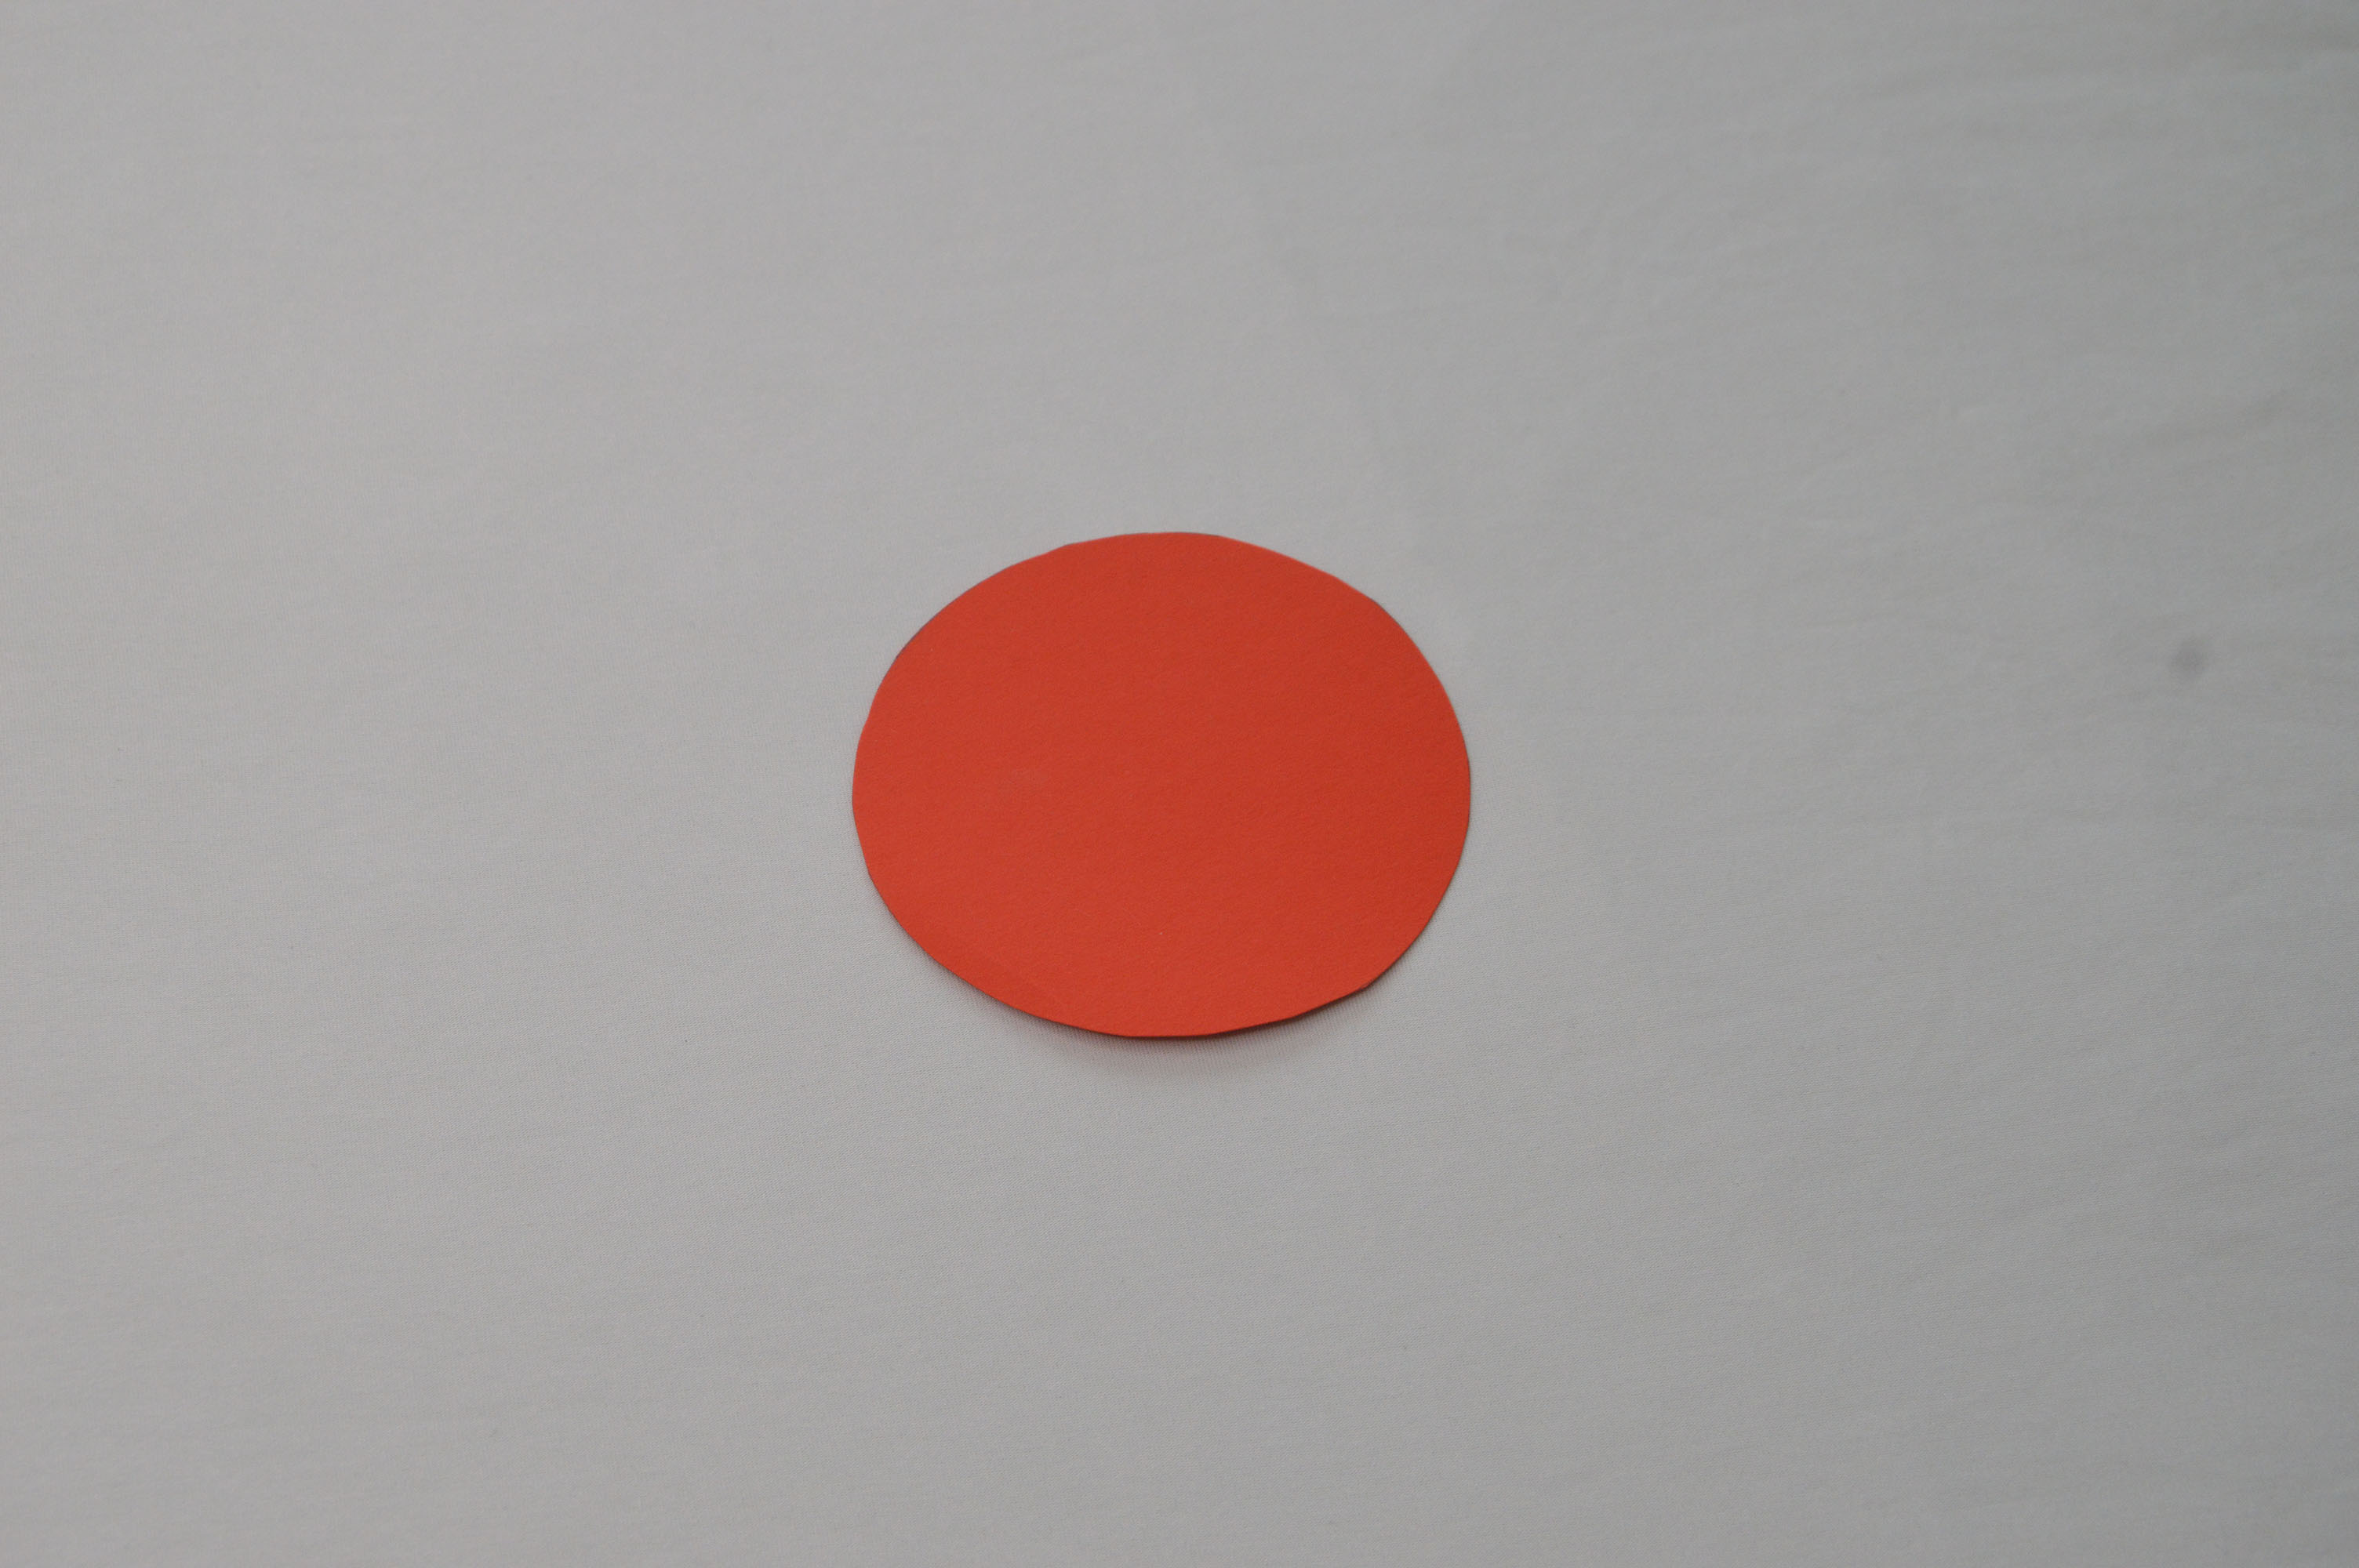
\includegraphics[width=.20\linewidth]{images/train01.jpg}
		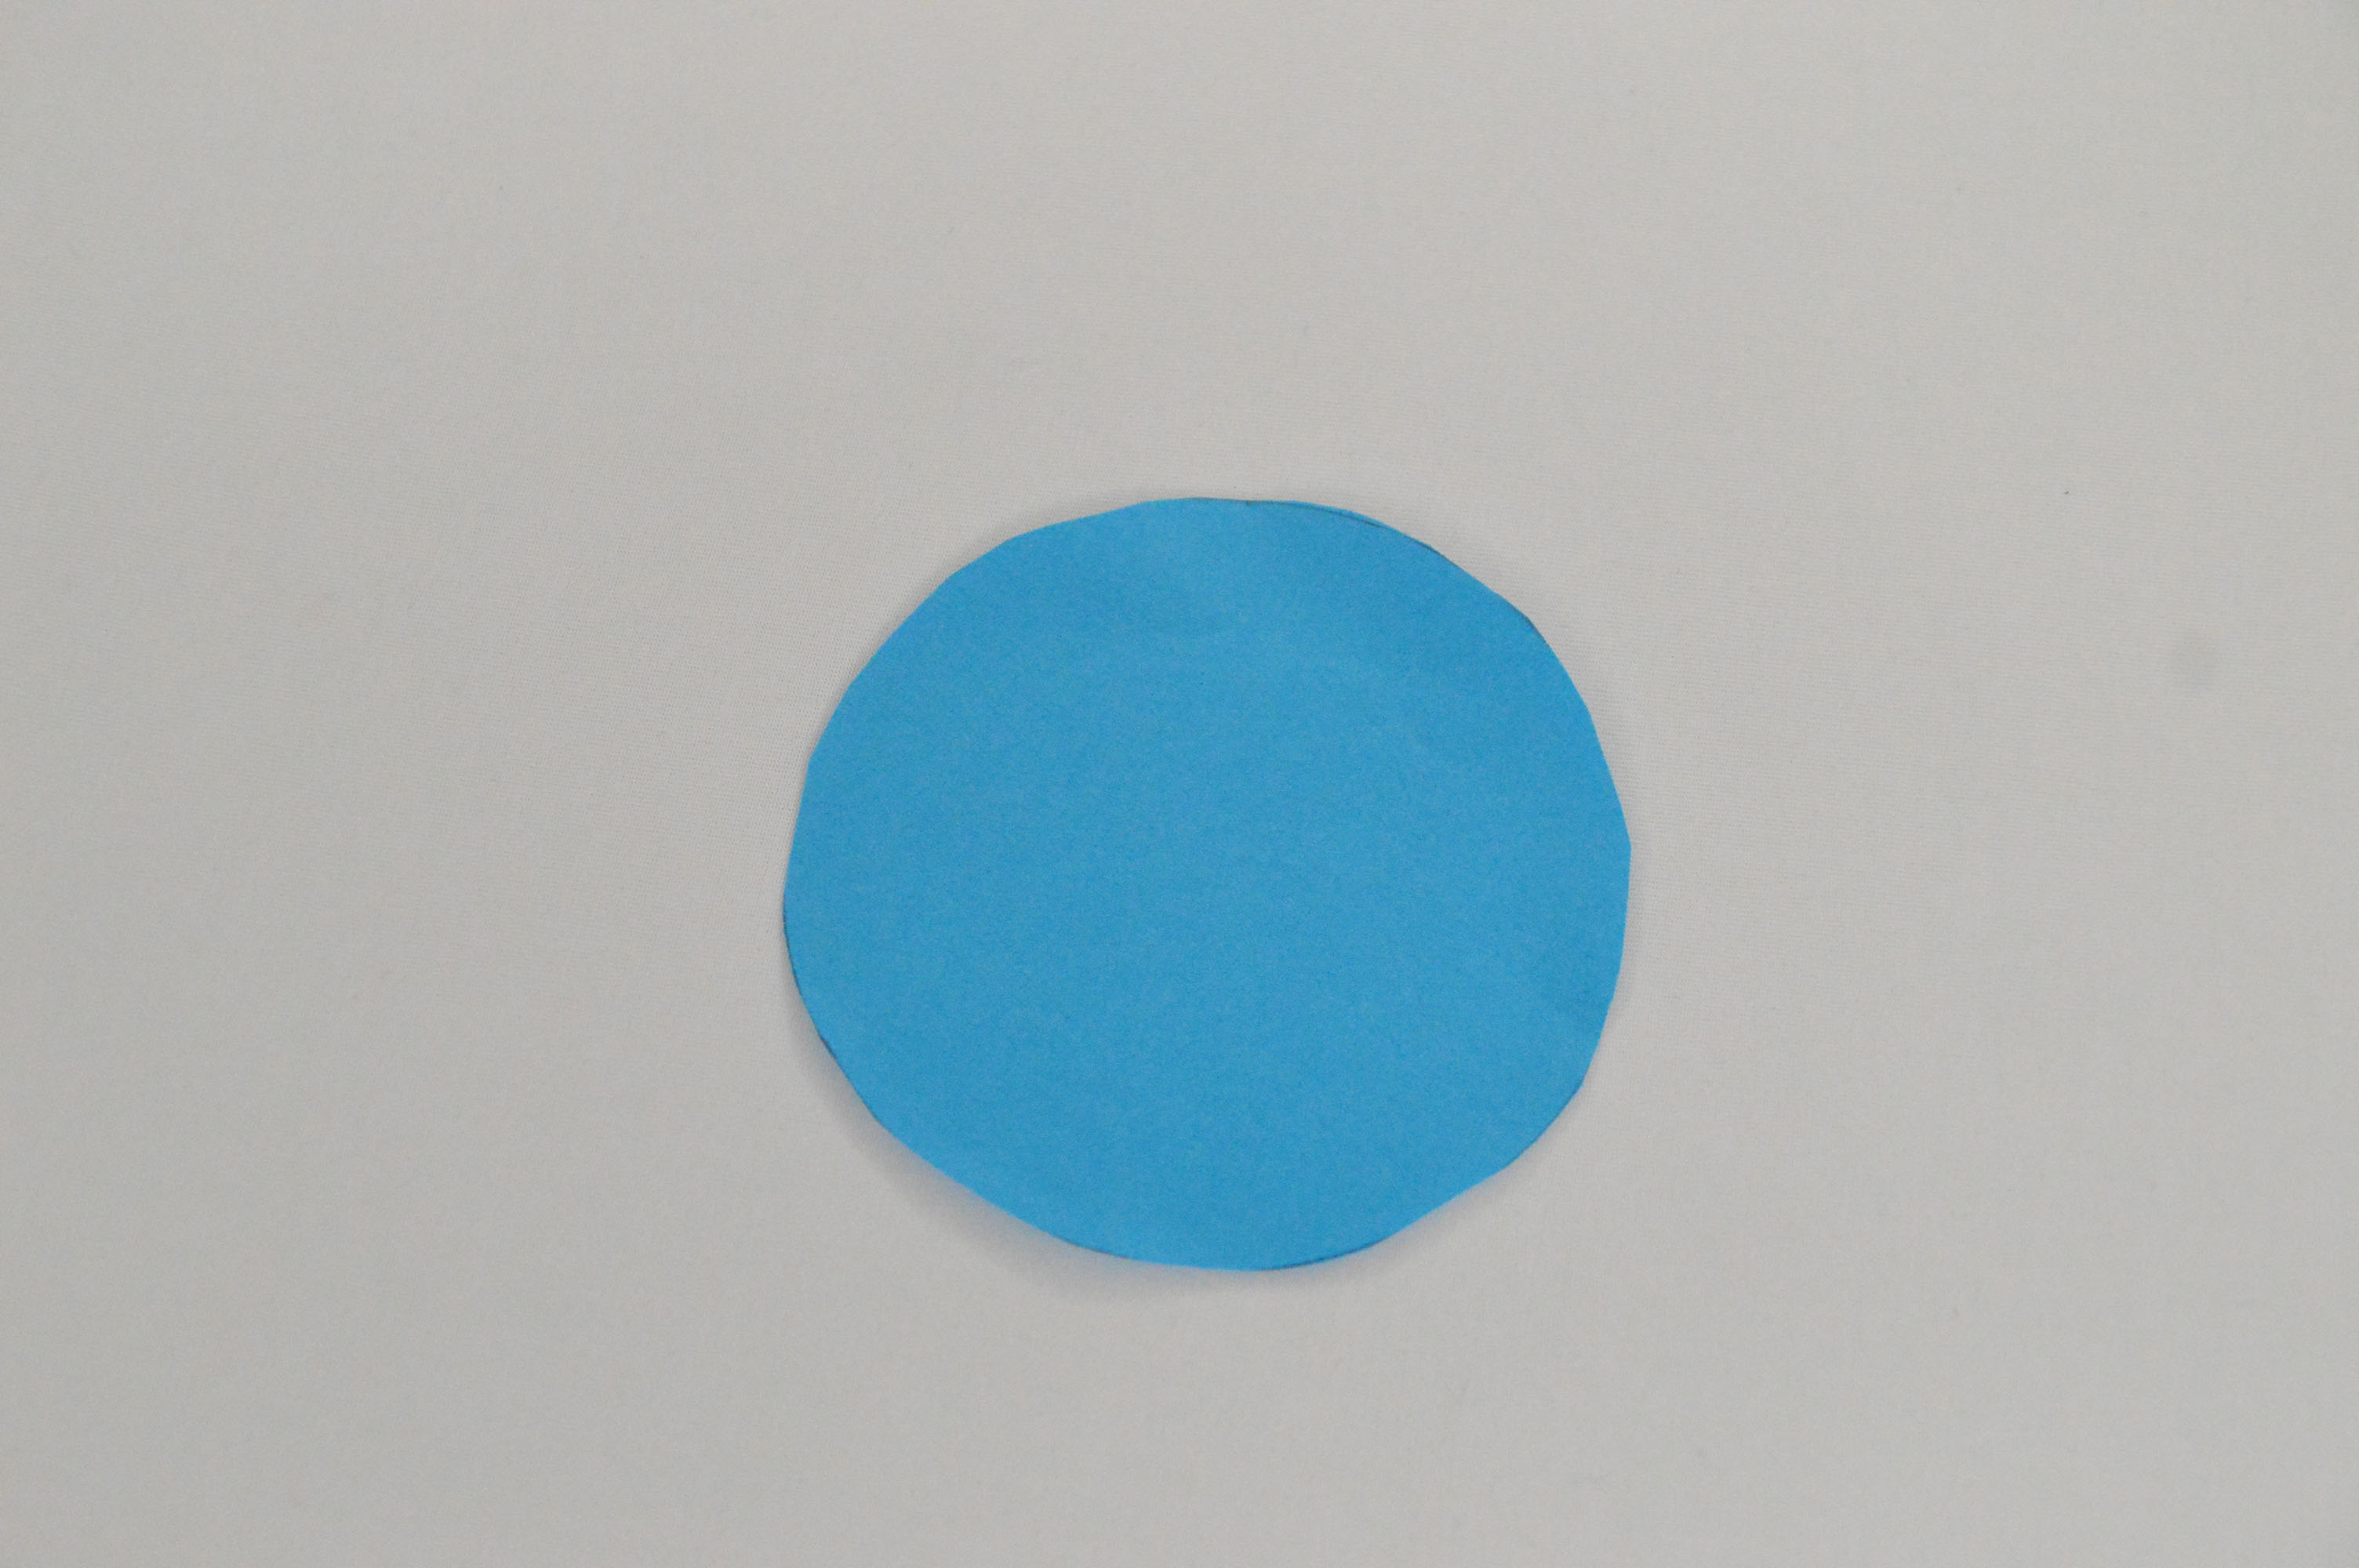
\includegraphics[width=.20\linewidth]{images/train02.jpg}
		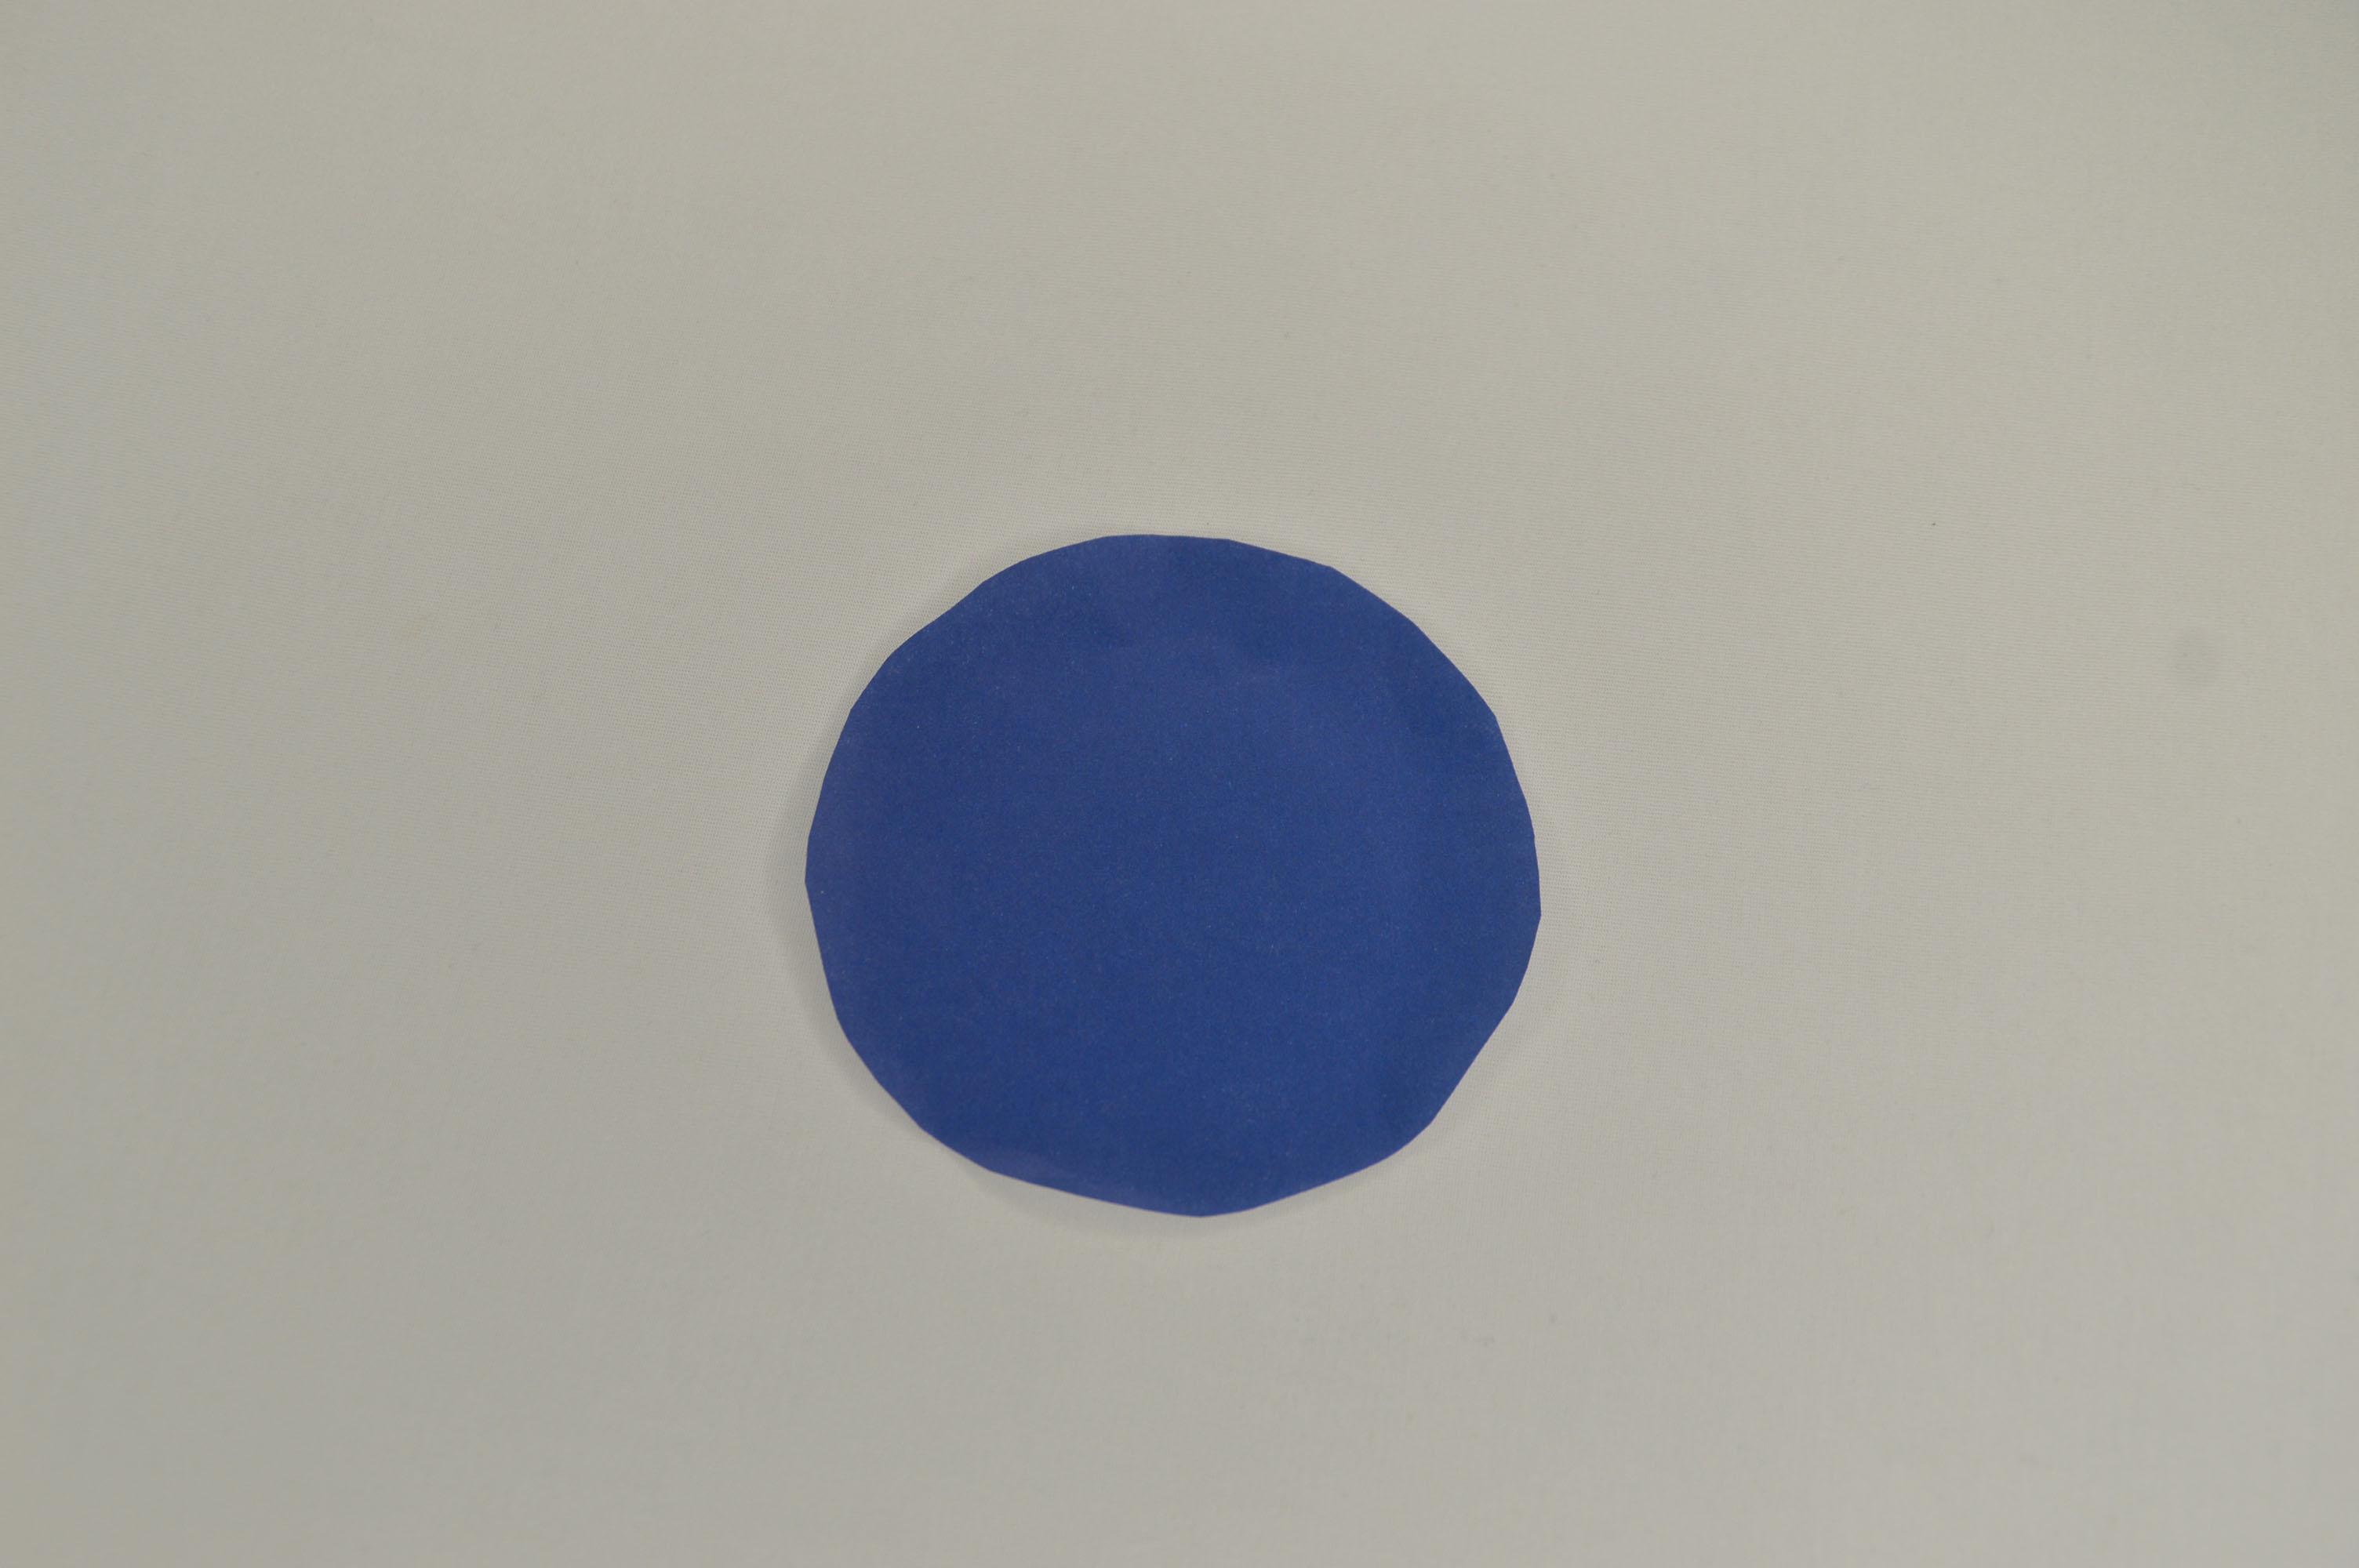
\includegraphics[width=.20\linewidth]{images/train03.jpg}
		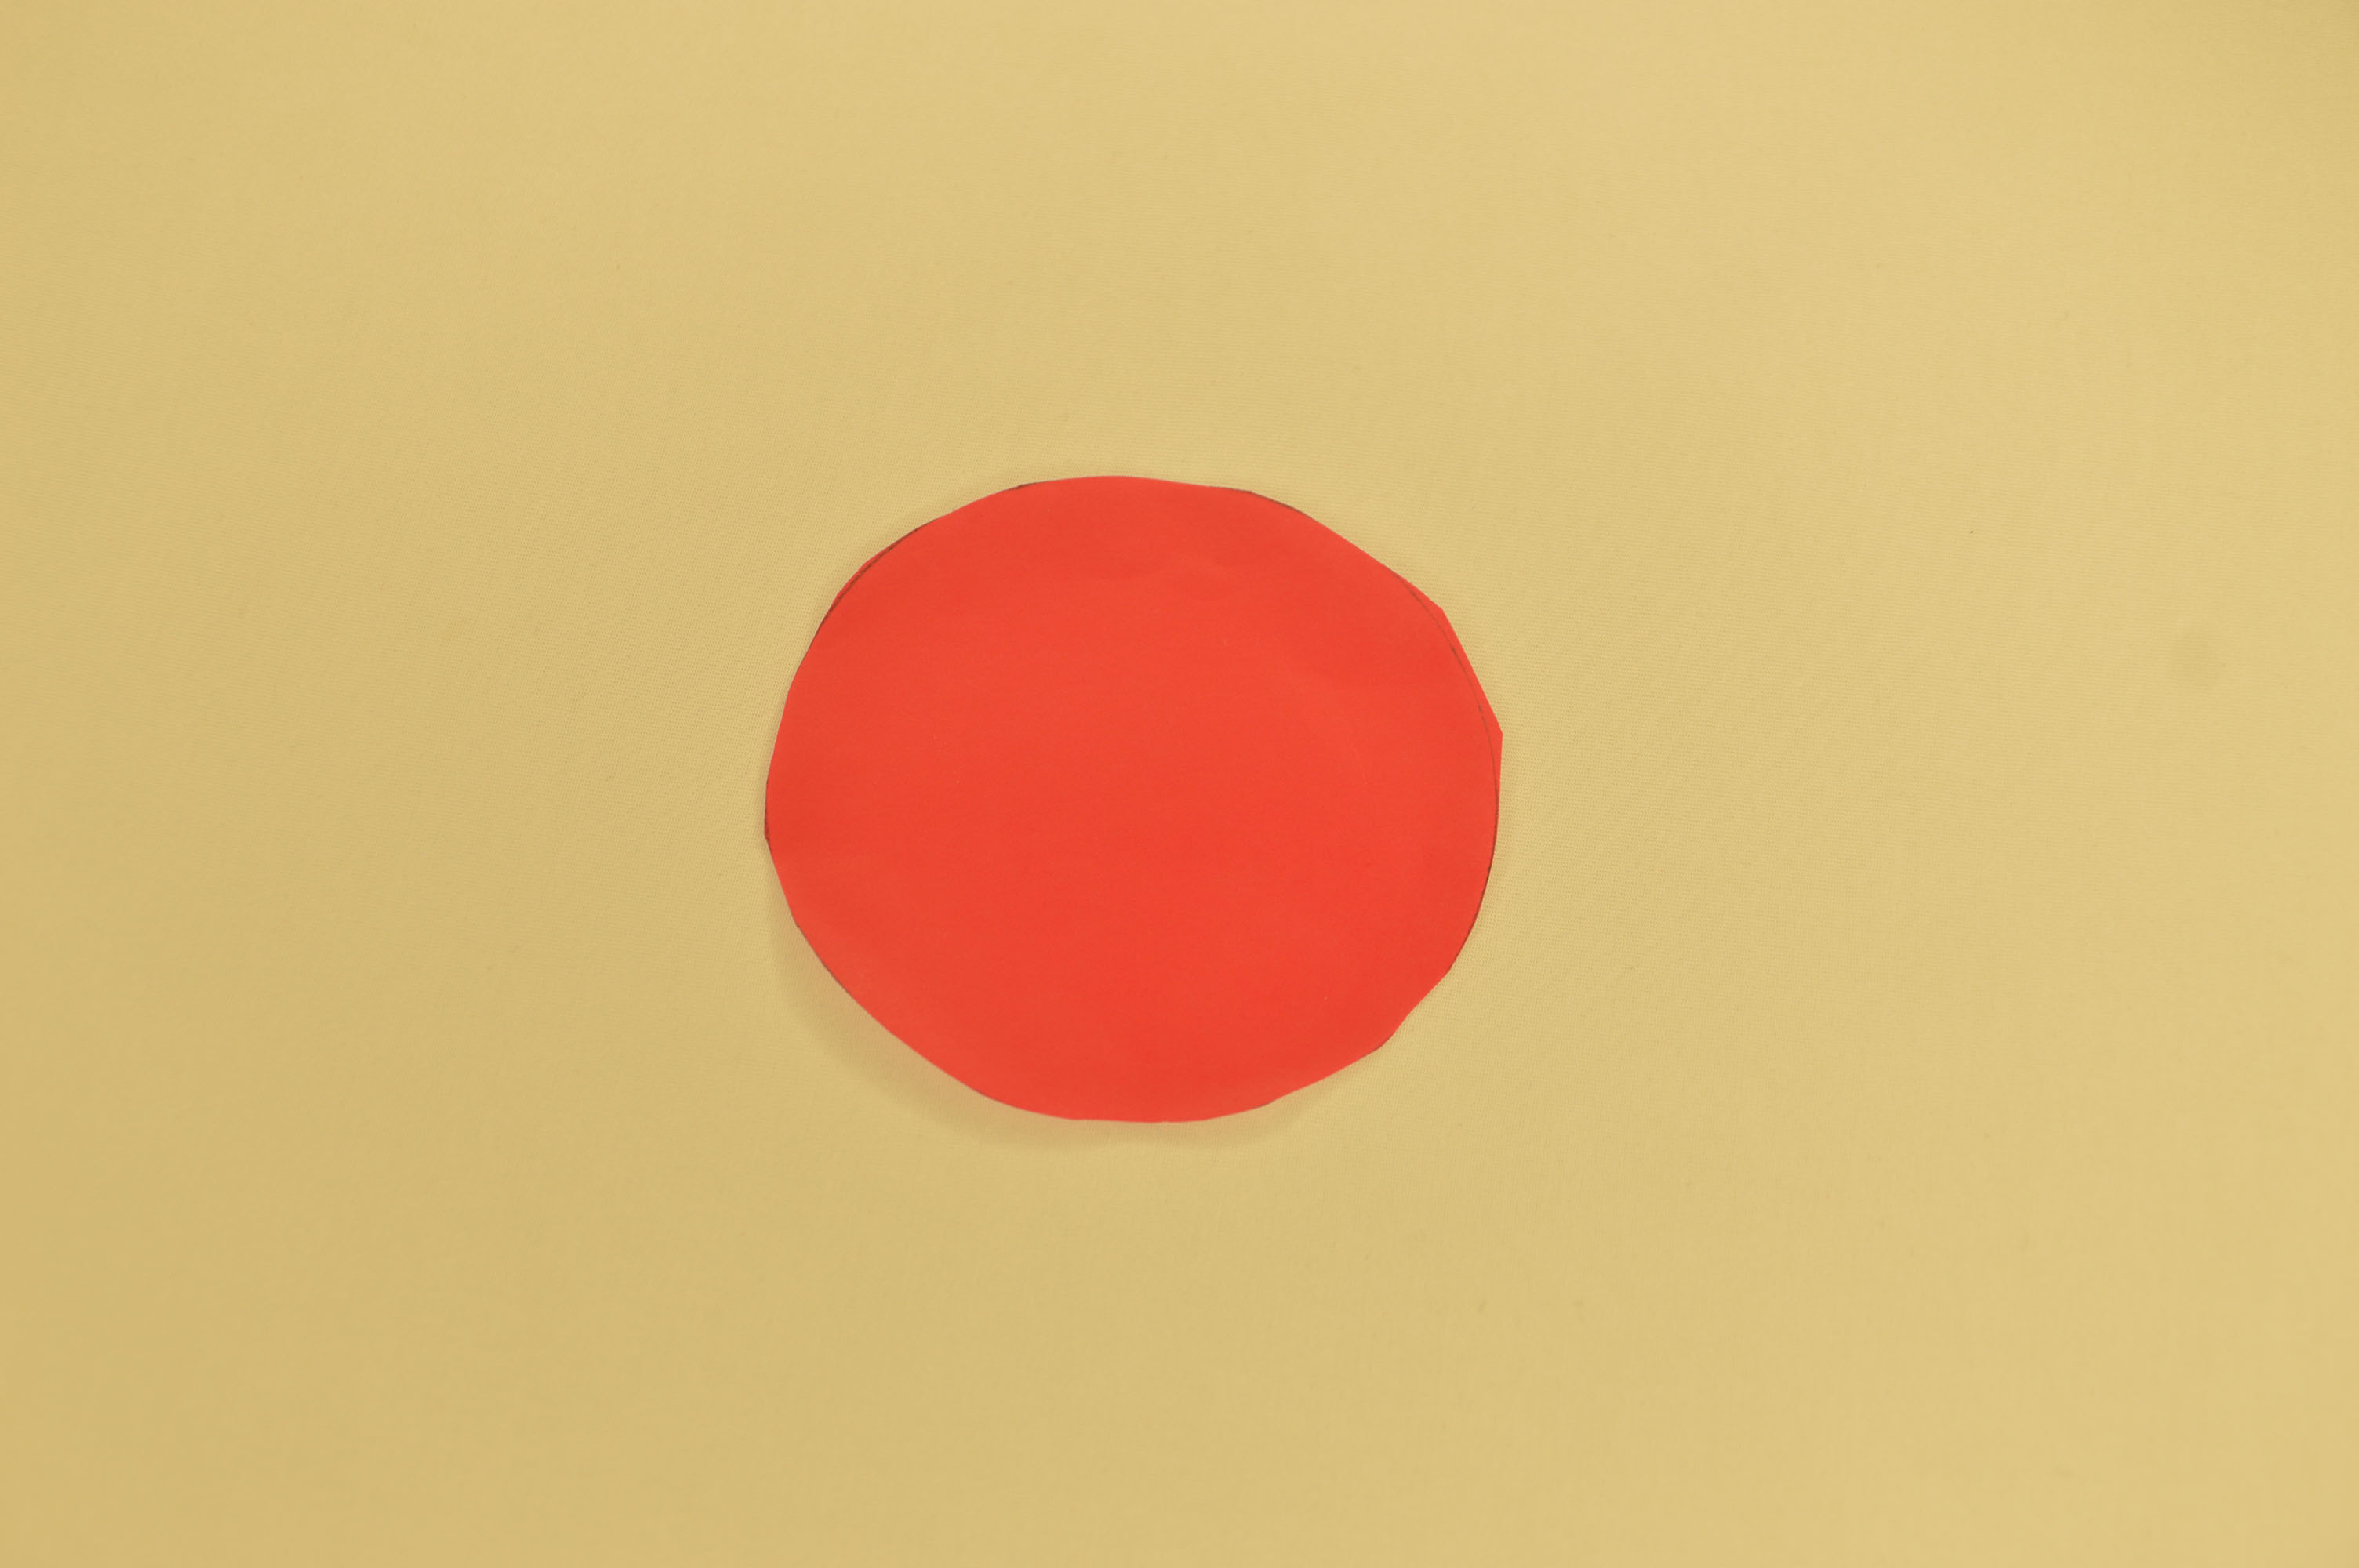
\includegraphics[width=.20\linewidth]{images/train04.jpg} \\
		\vspace{3pt}
		
\includegraphics[width=.20\linewidth]{images/train05.jpg}
		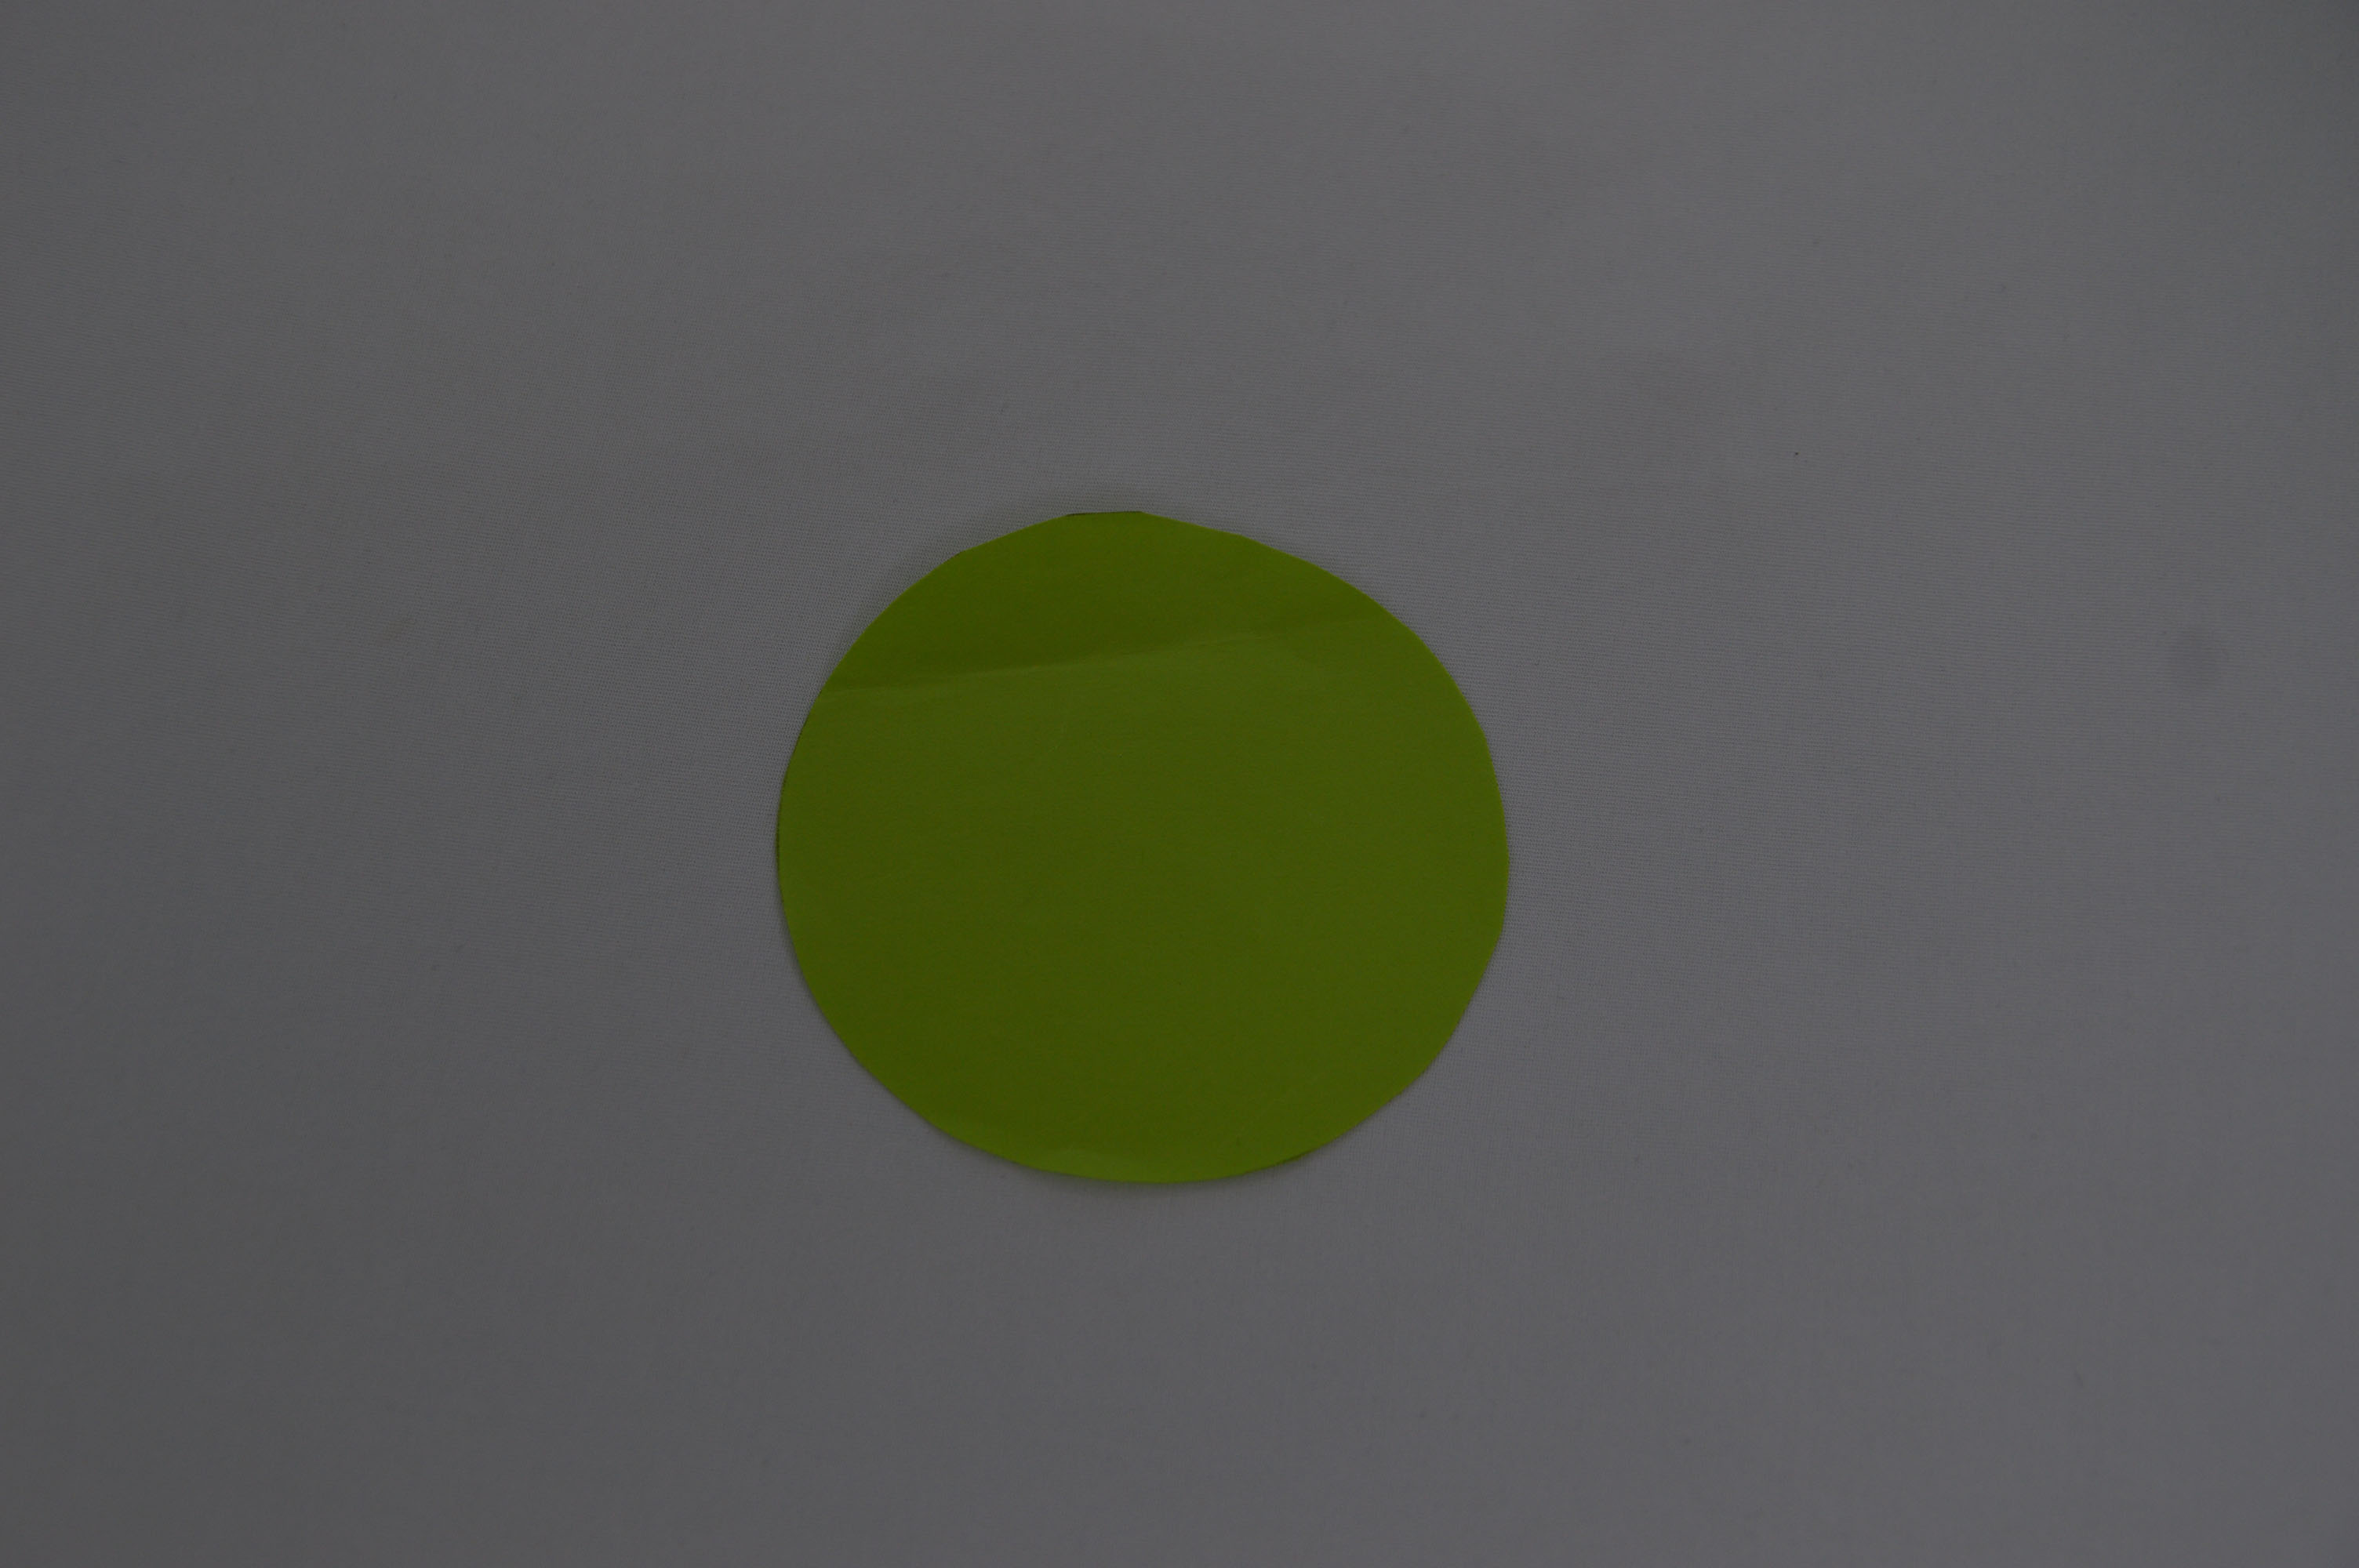
\includegraphics[width=.20\linewidth]{images/train06.jpg}
		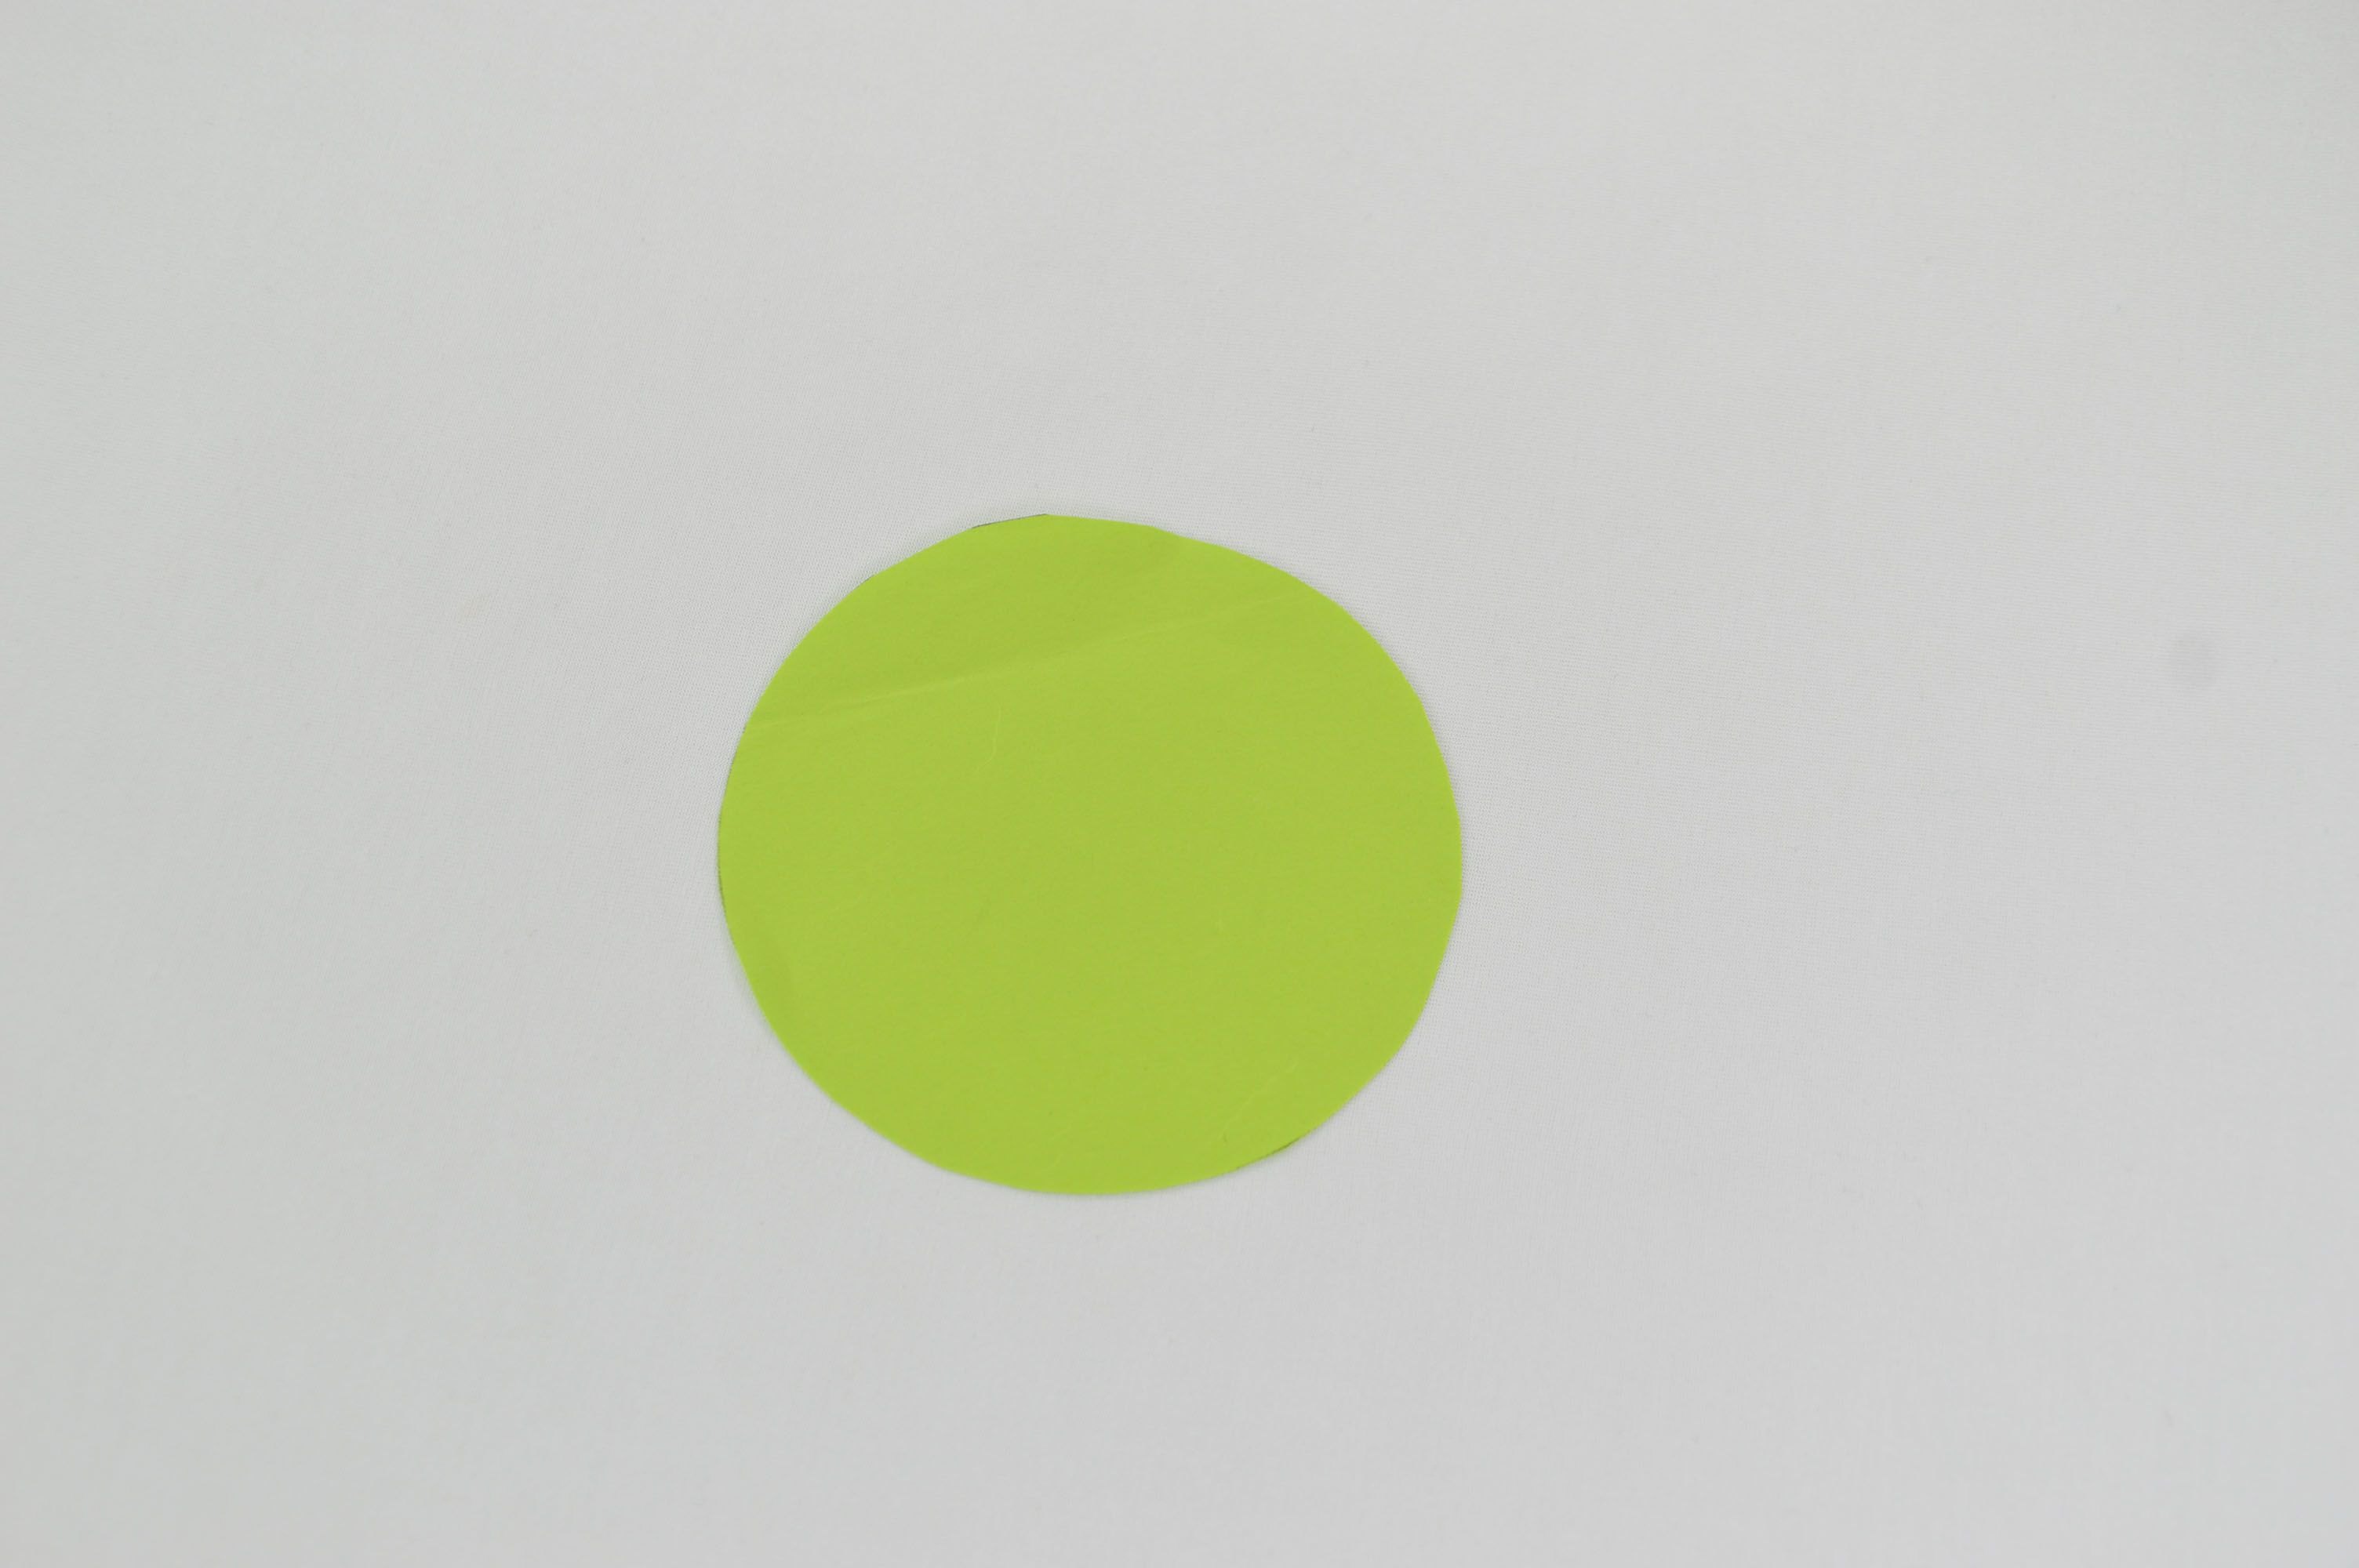
\includegraphics[width=.20\linewidth]{images/train07.jpg}
		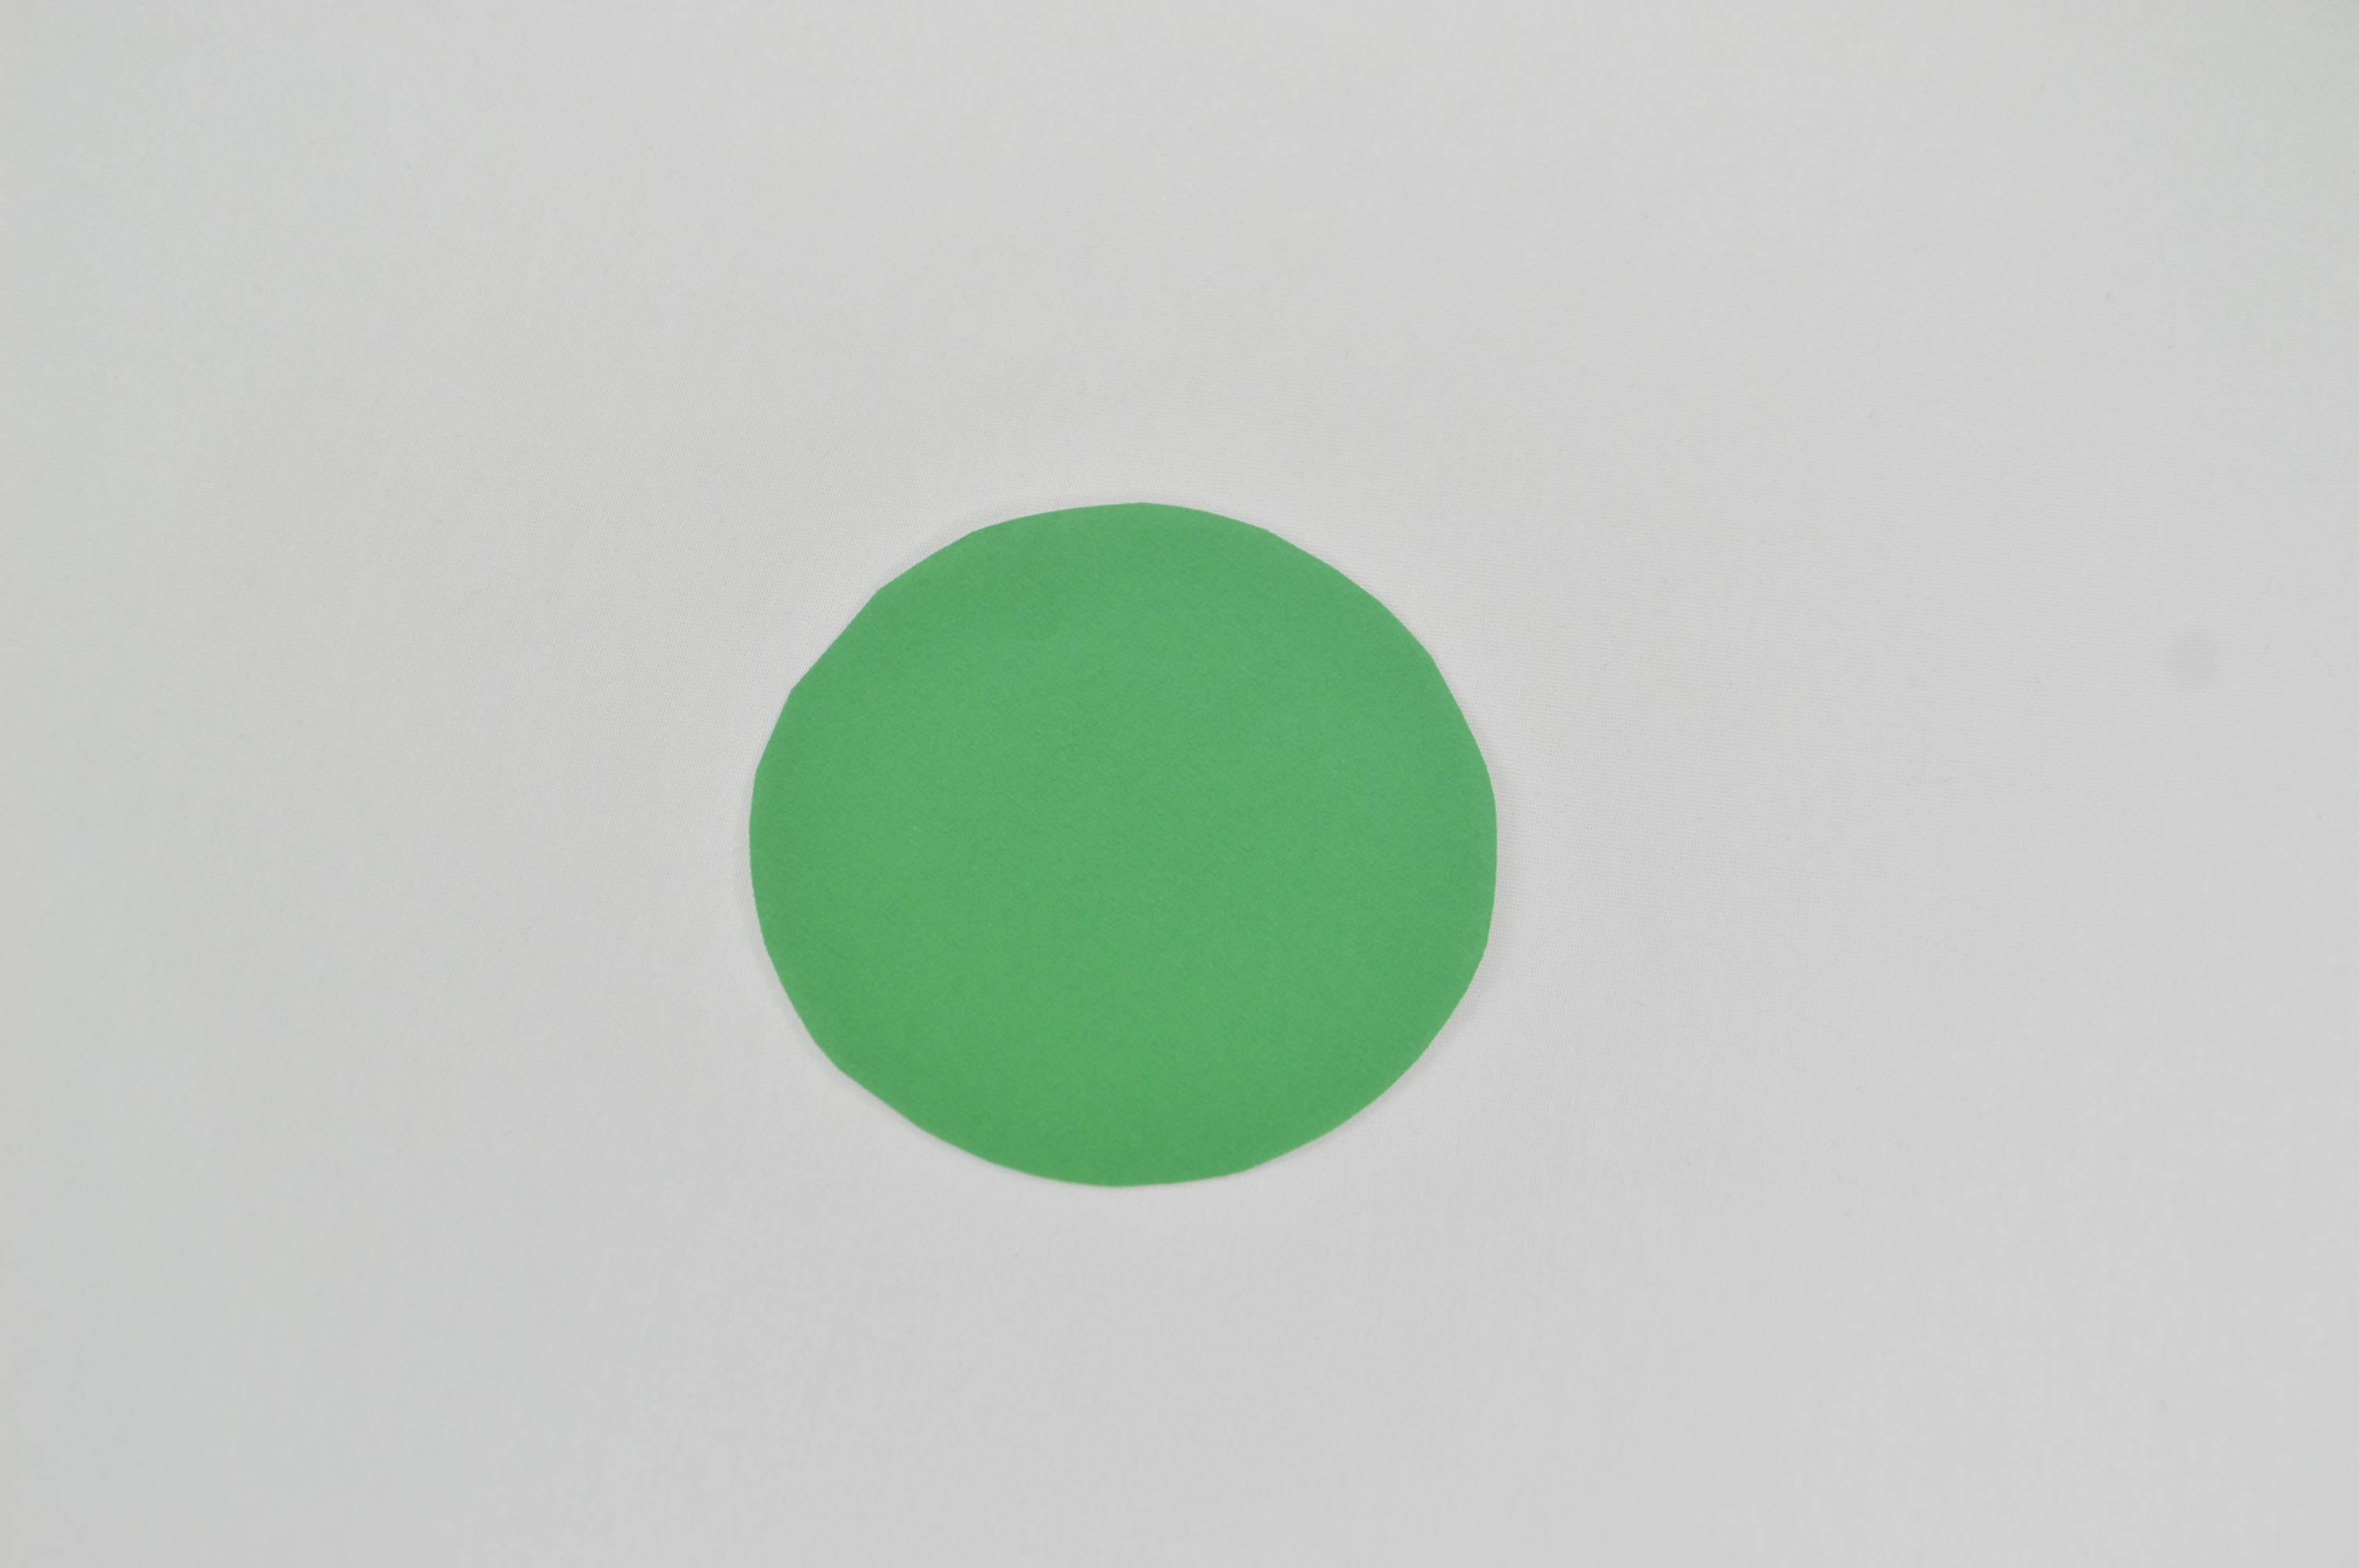
\includegraphics[width=.20\linewidth]{images/train08.jpg}
		\caption{Training set}
	\end{figure}

	Those images were then used to train our colour classifier.
	
	For testing set we used different images of single coloured cylinders with roughly the same diameter. A subset of the test images is included below.
	
	\begin{figure}[H]
		\centering
		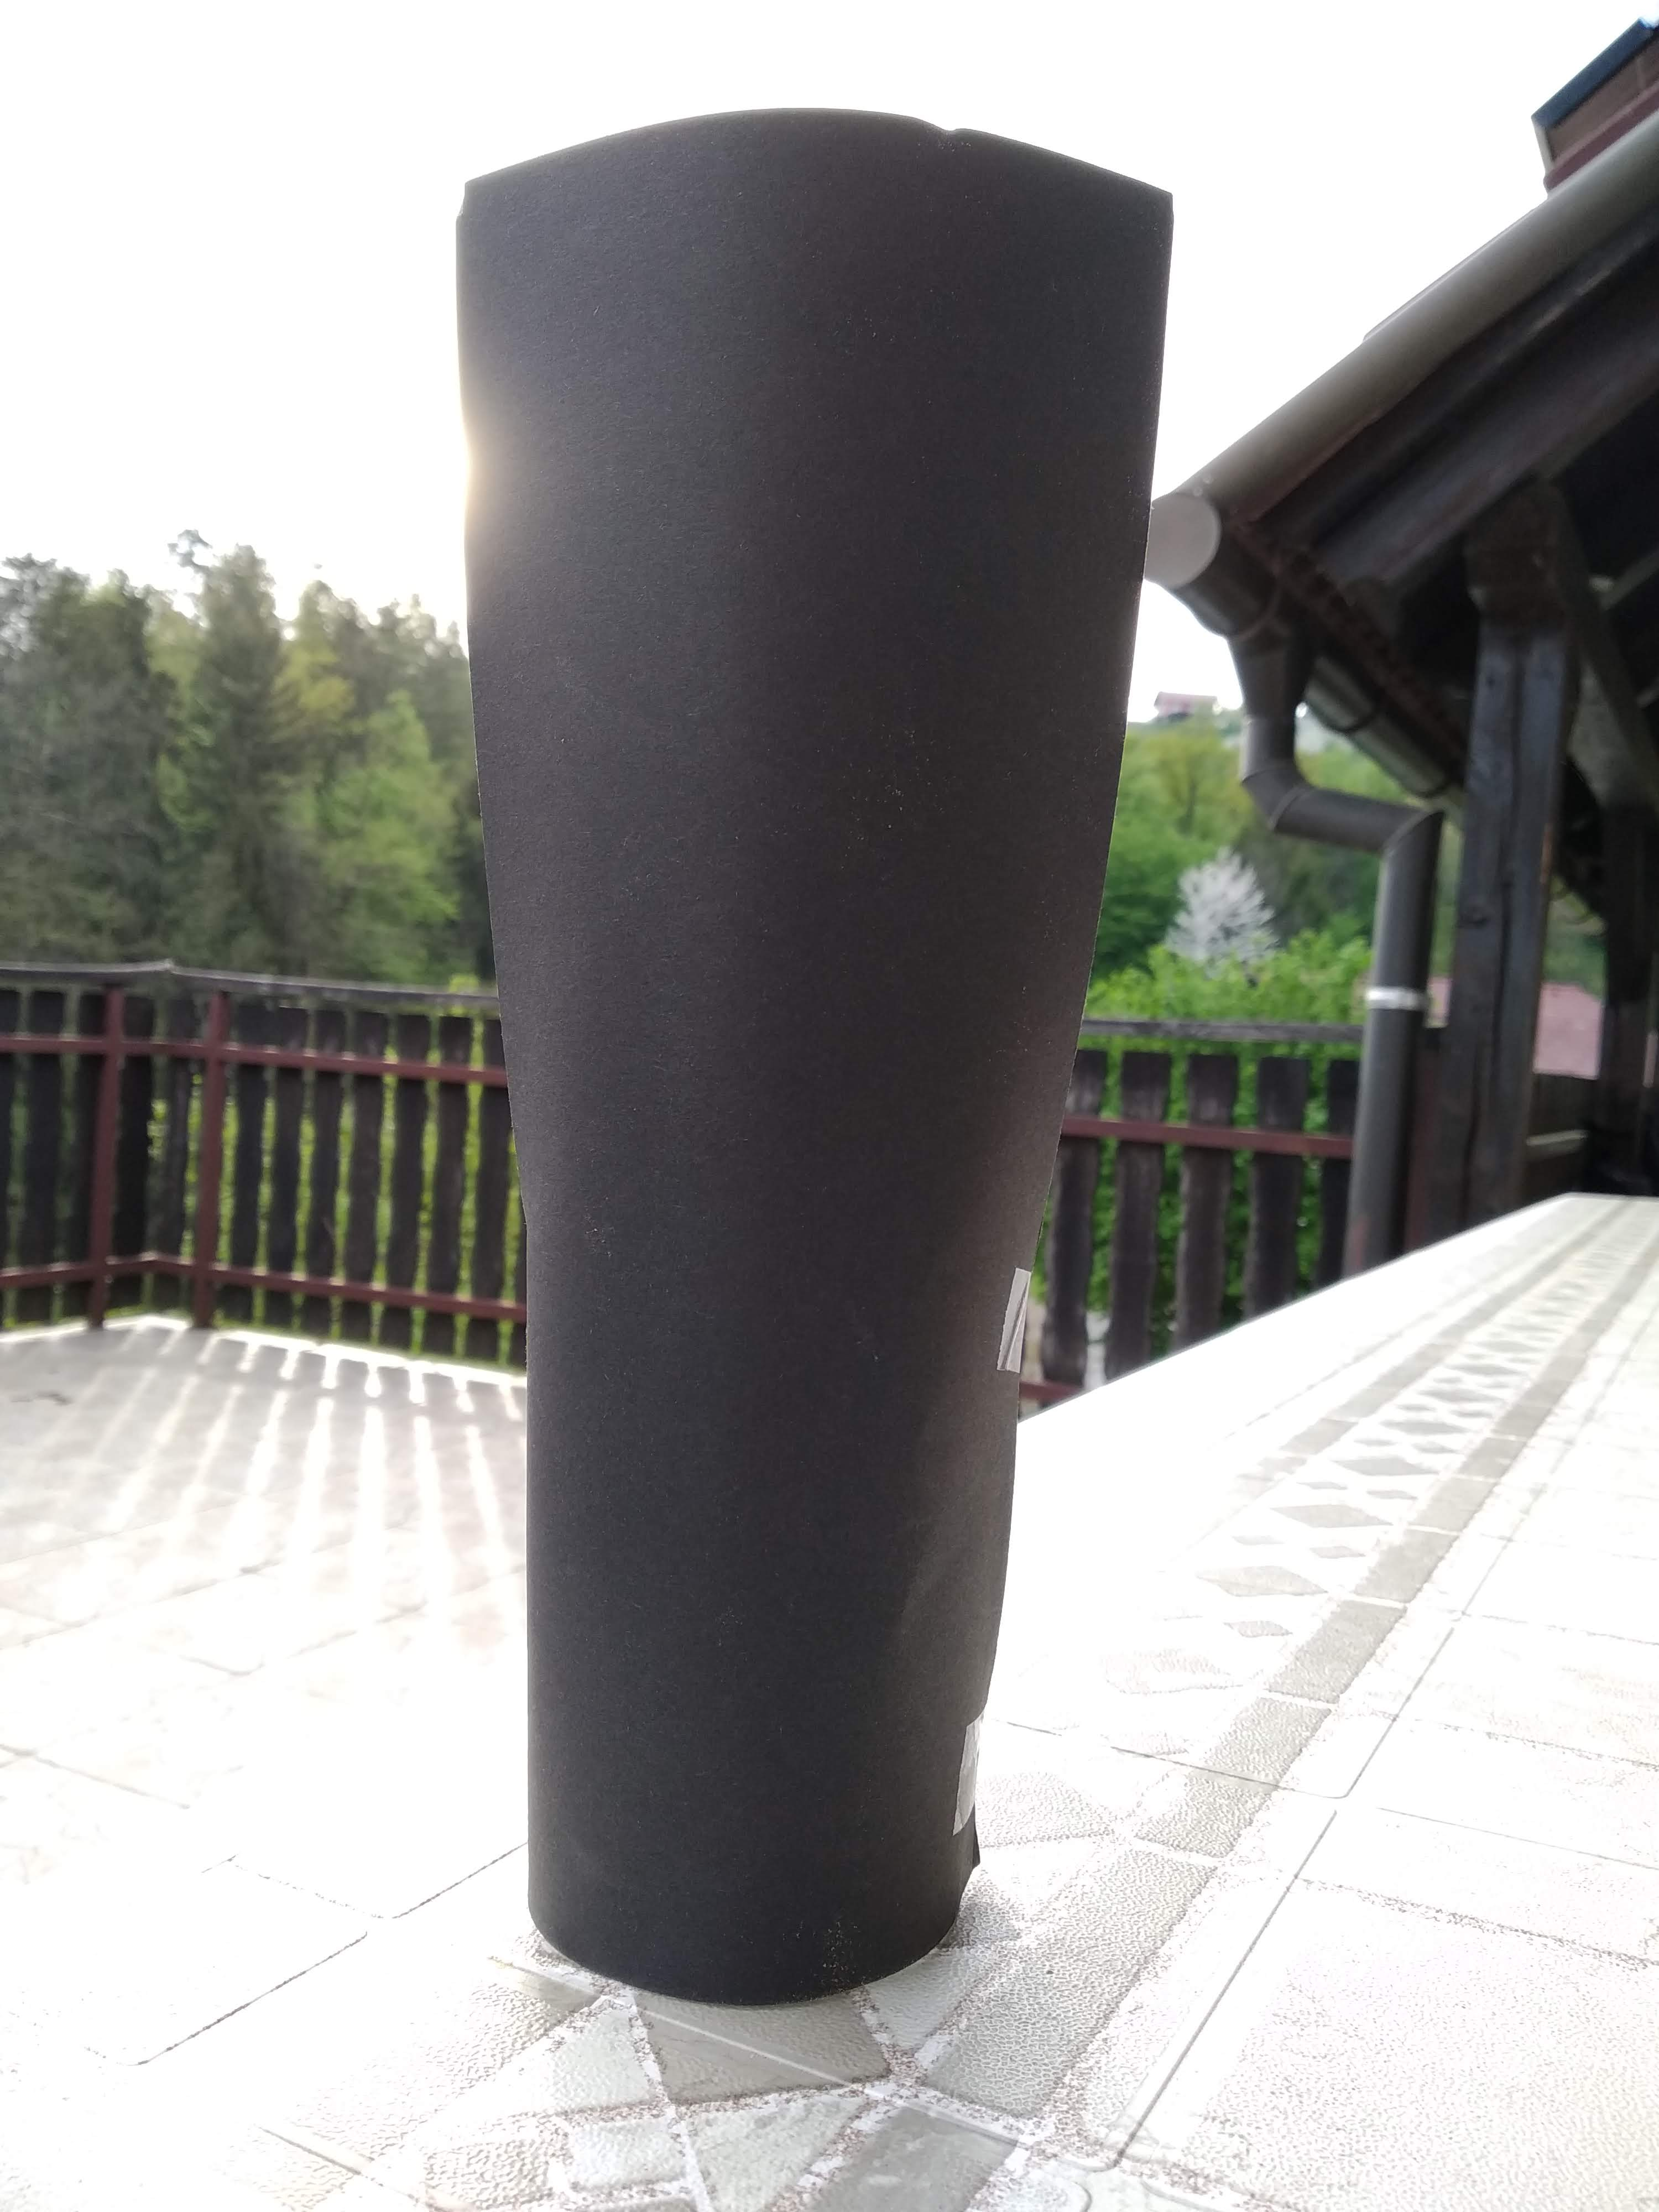
\includegraphics[width=.13\linewidth]{images/test01.jpg}
		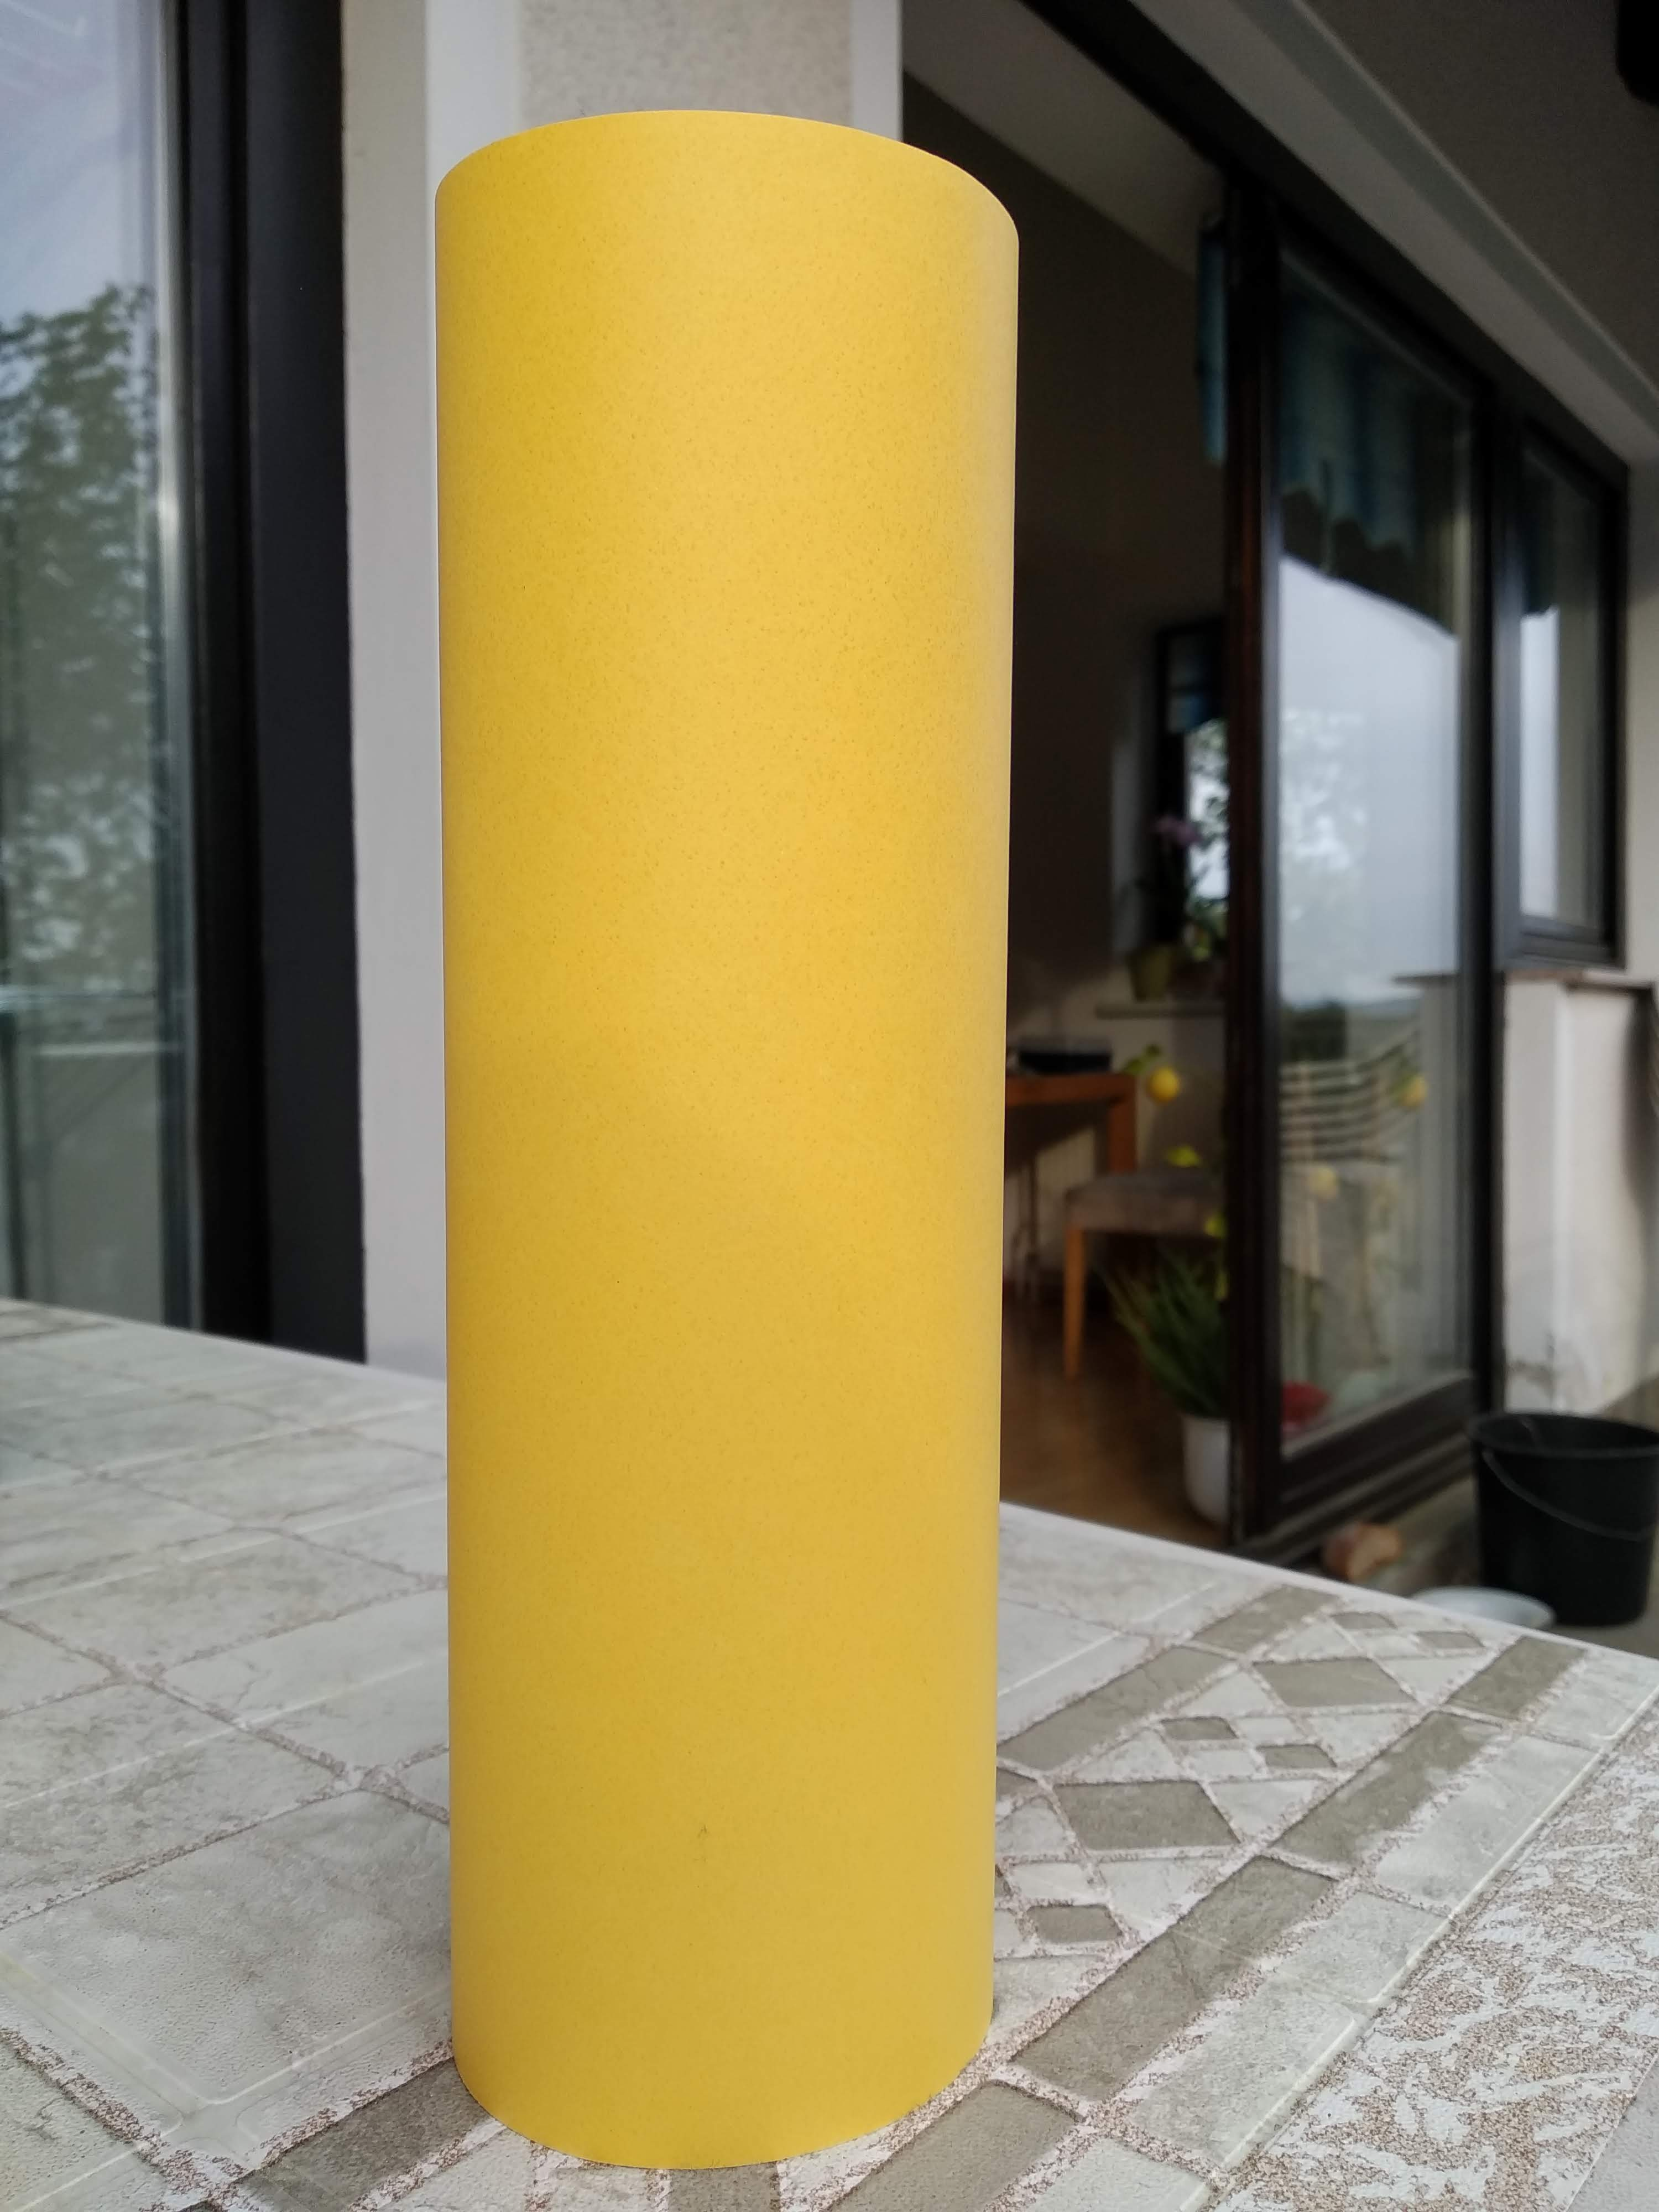
\includegraphics[width=.13\linewidth]{images/test02.jpg}
		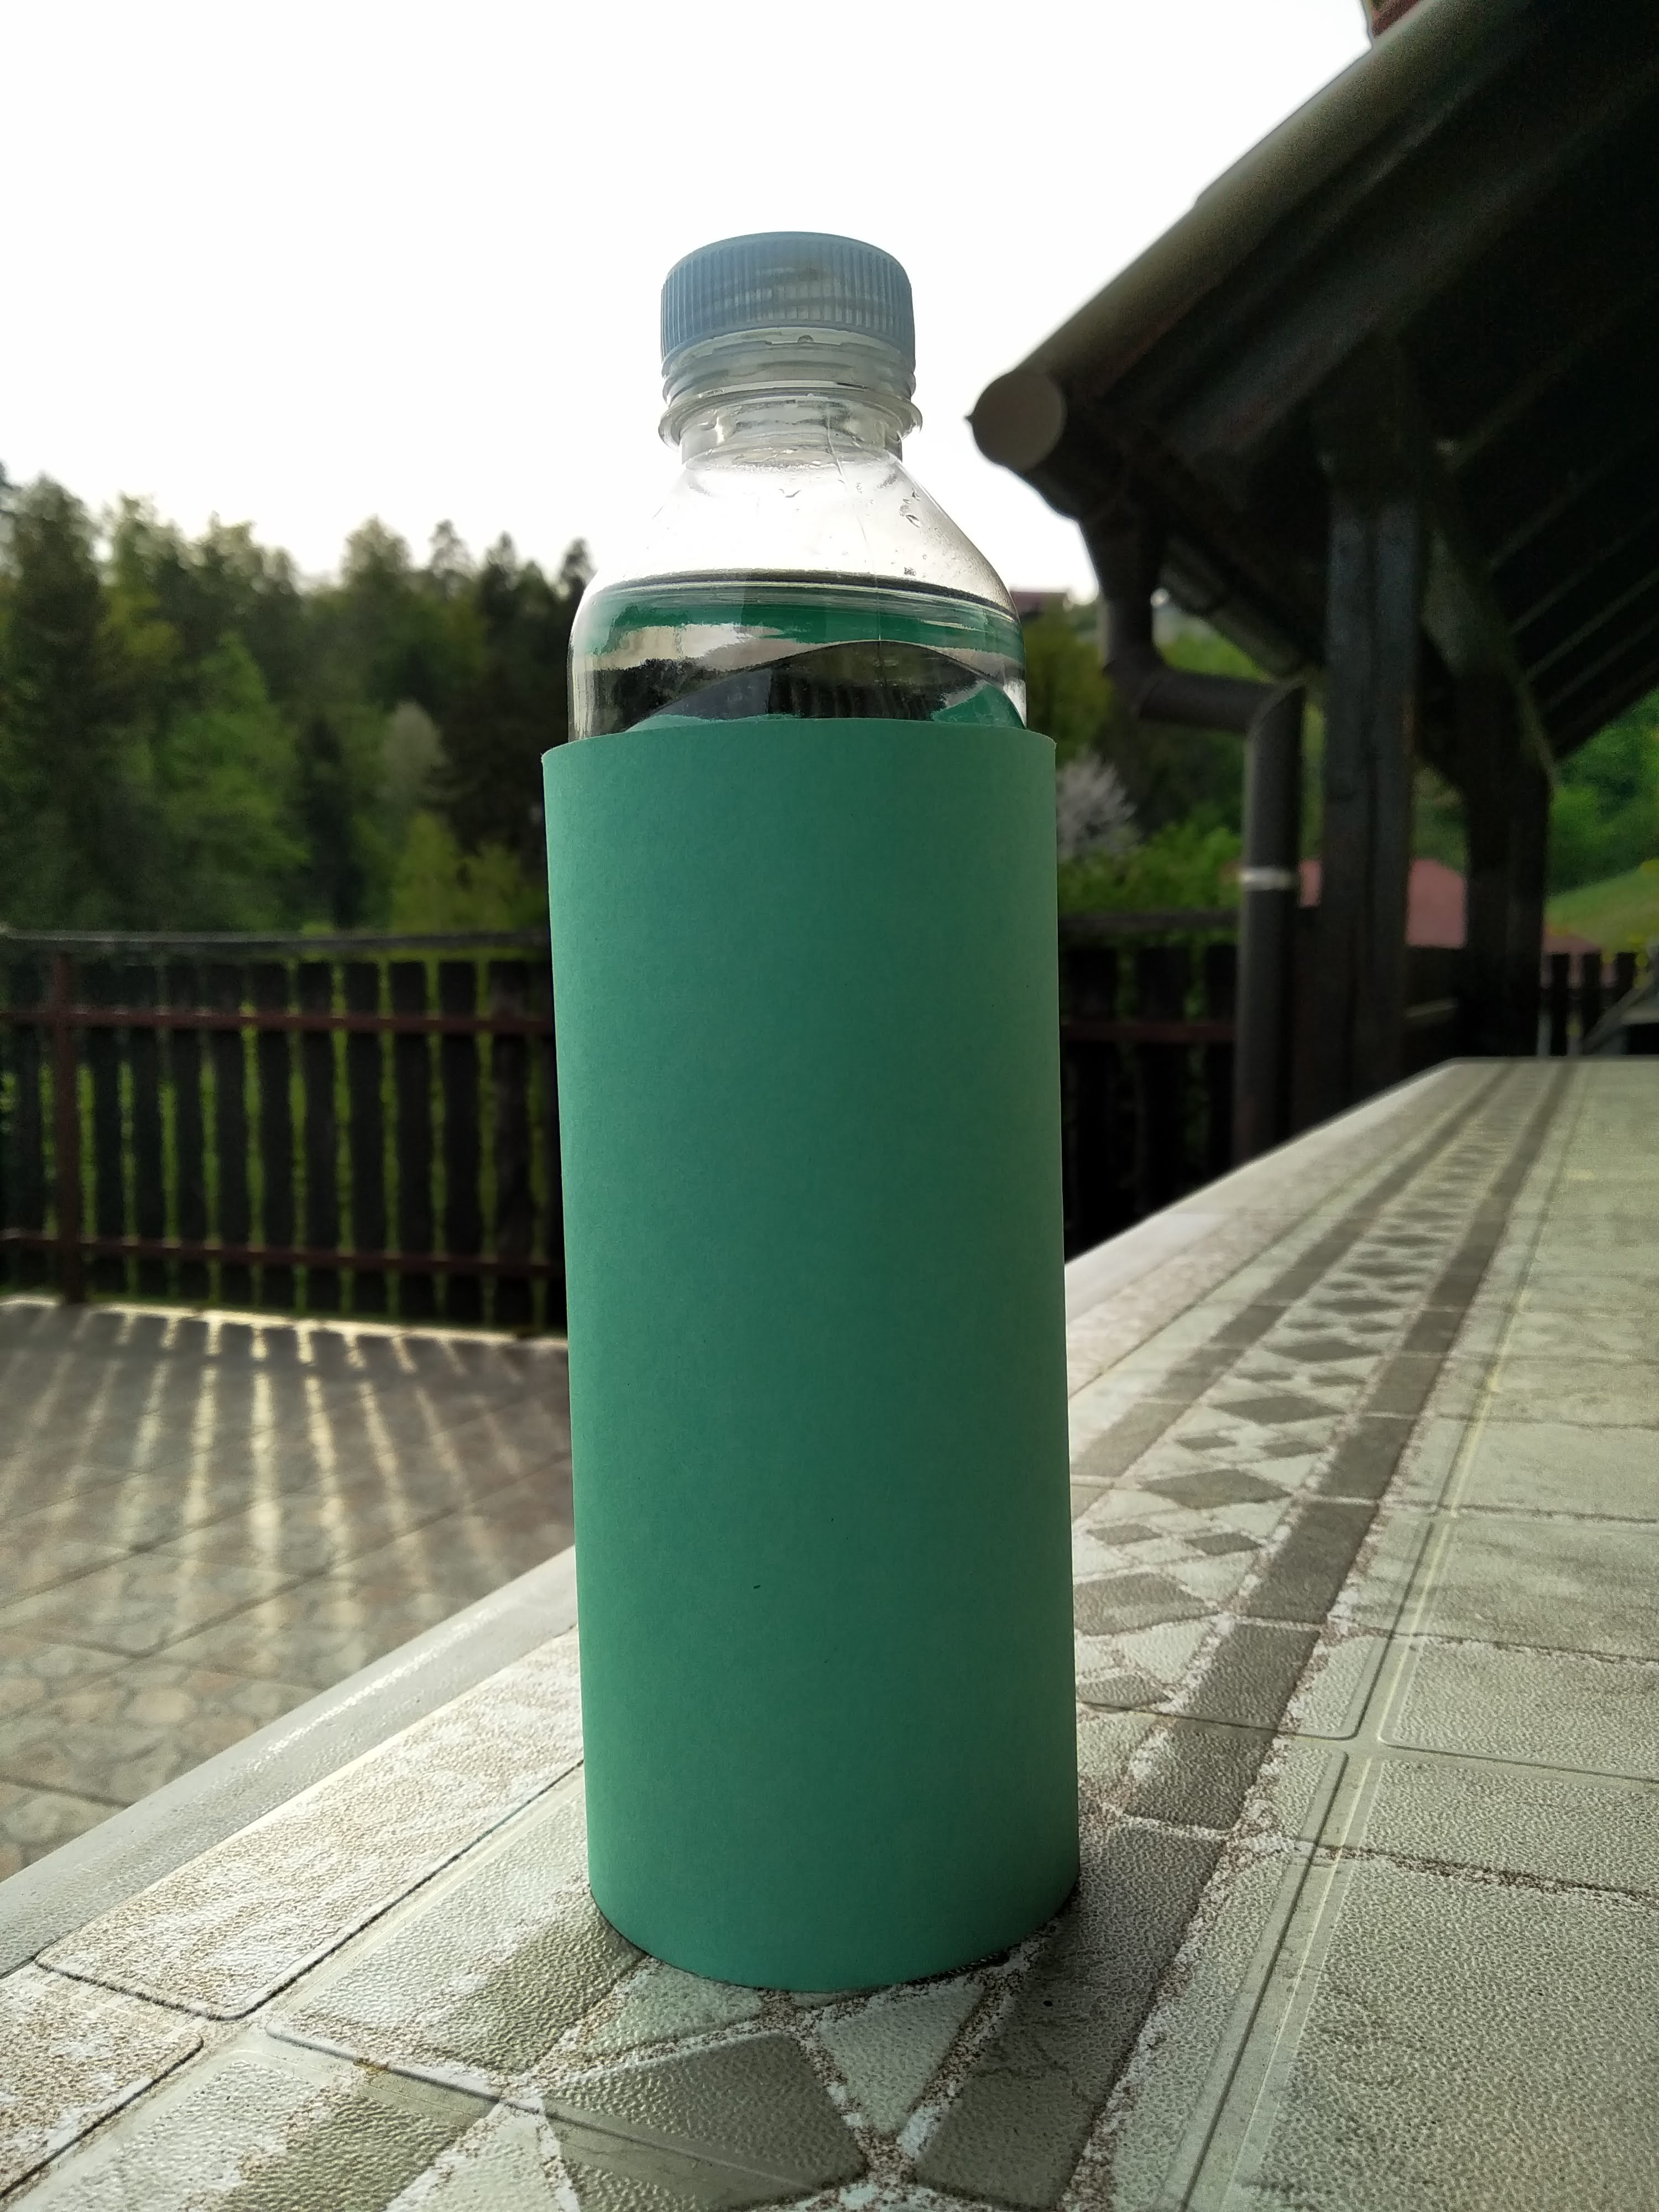
\includegraphics[width=.13\linewidth]{images/test03.jpg}
		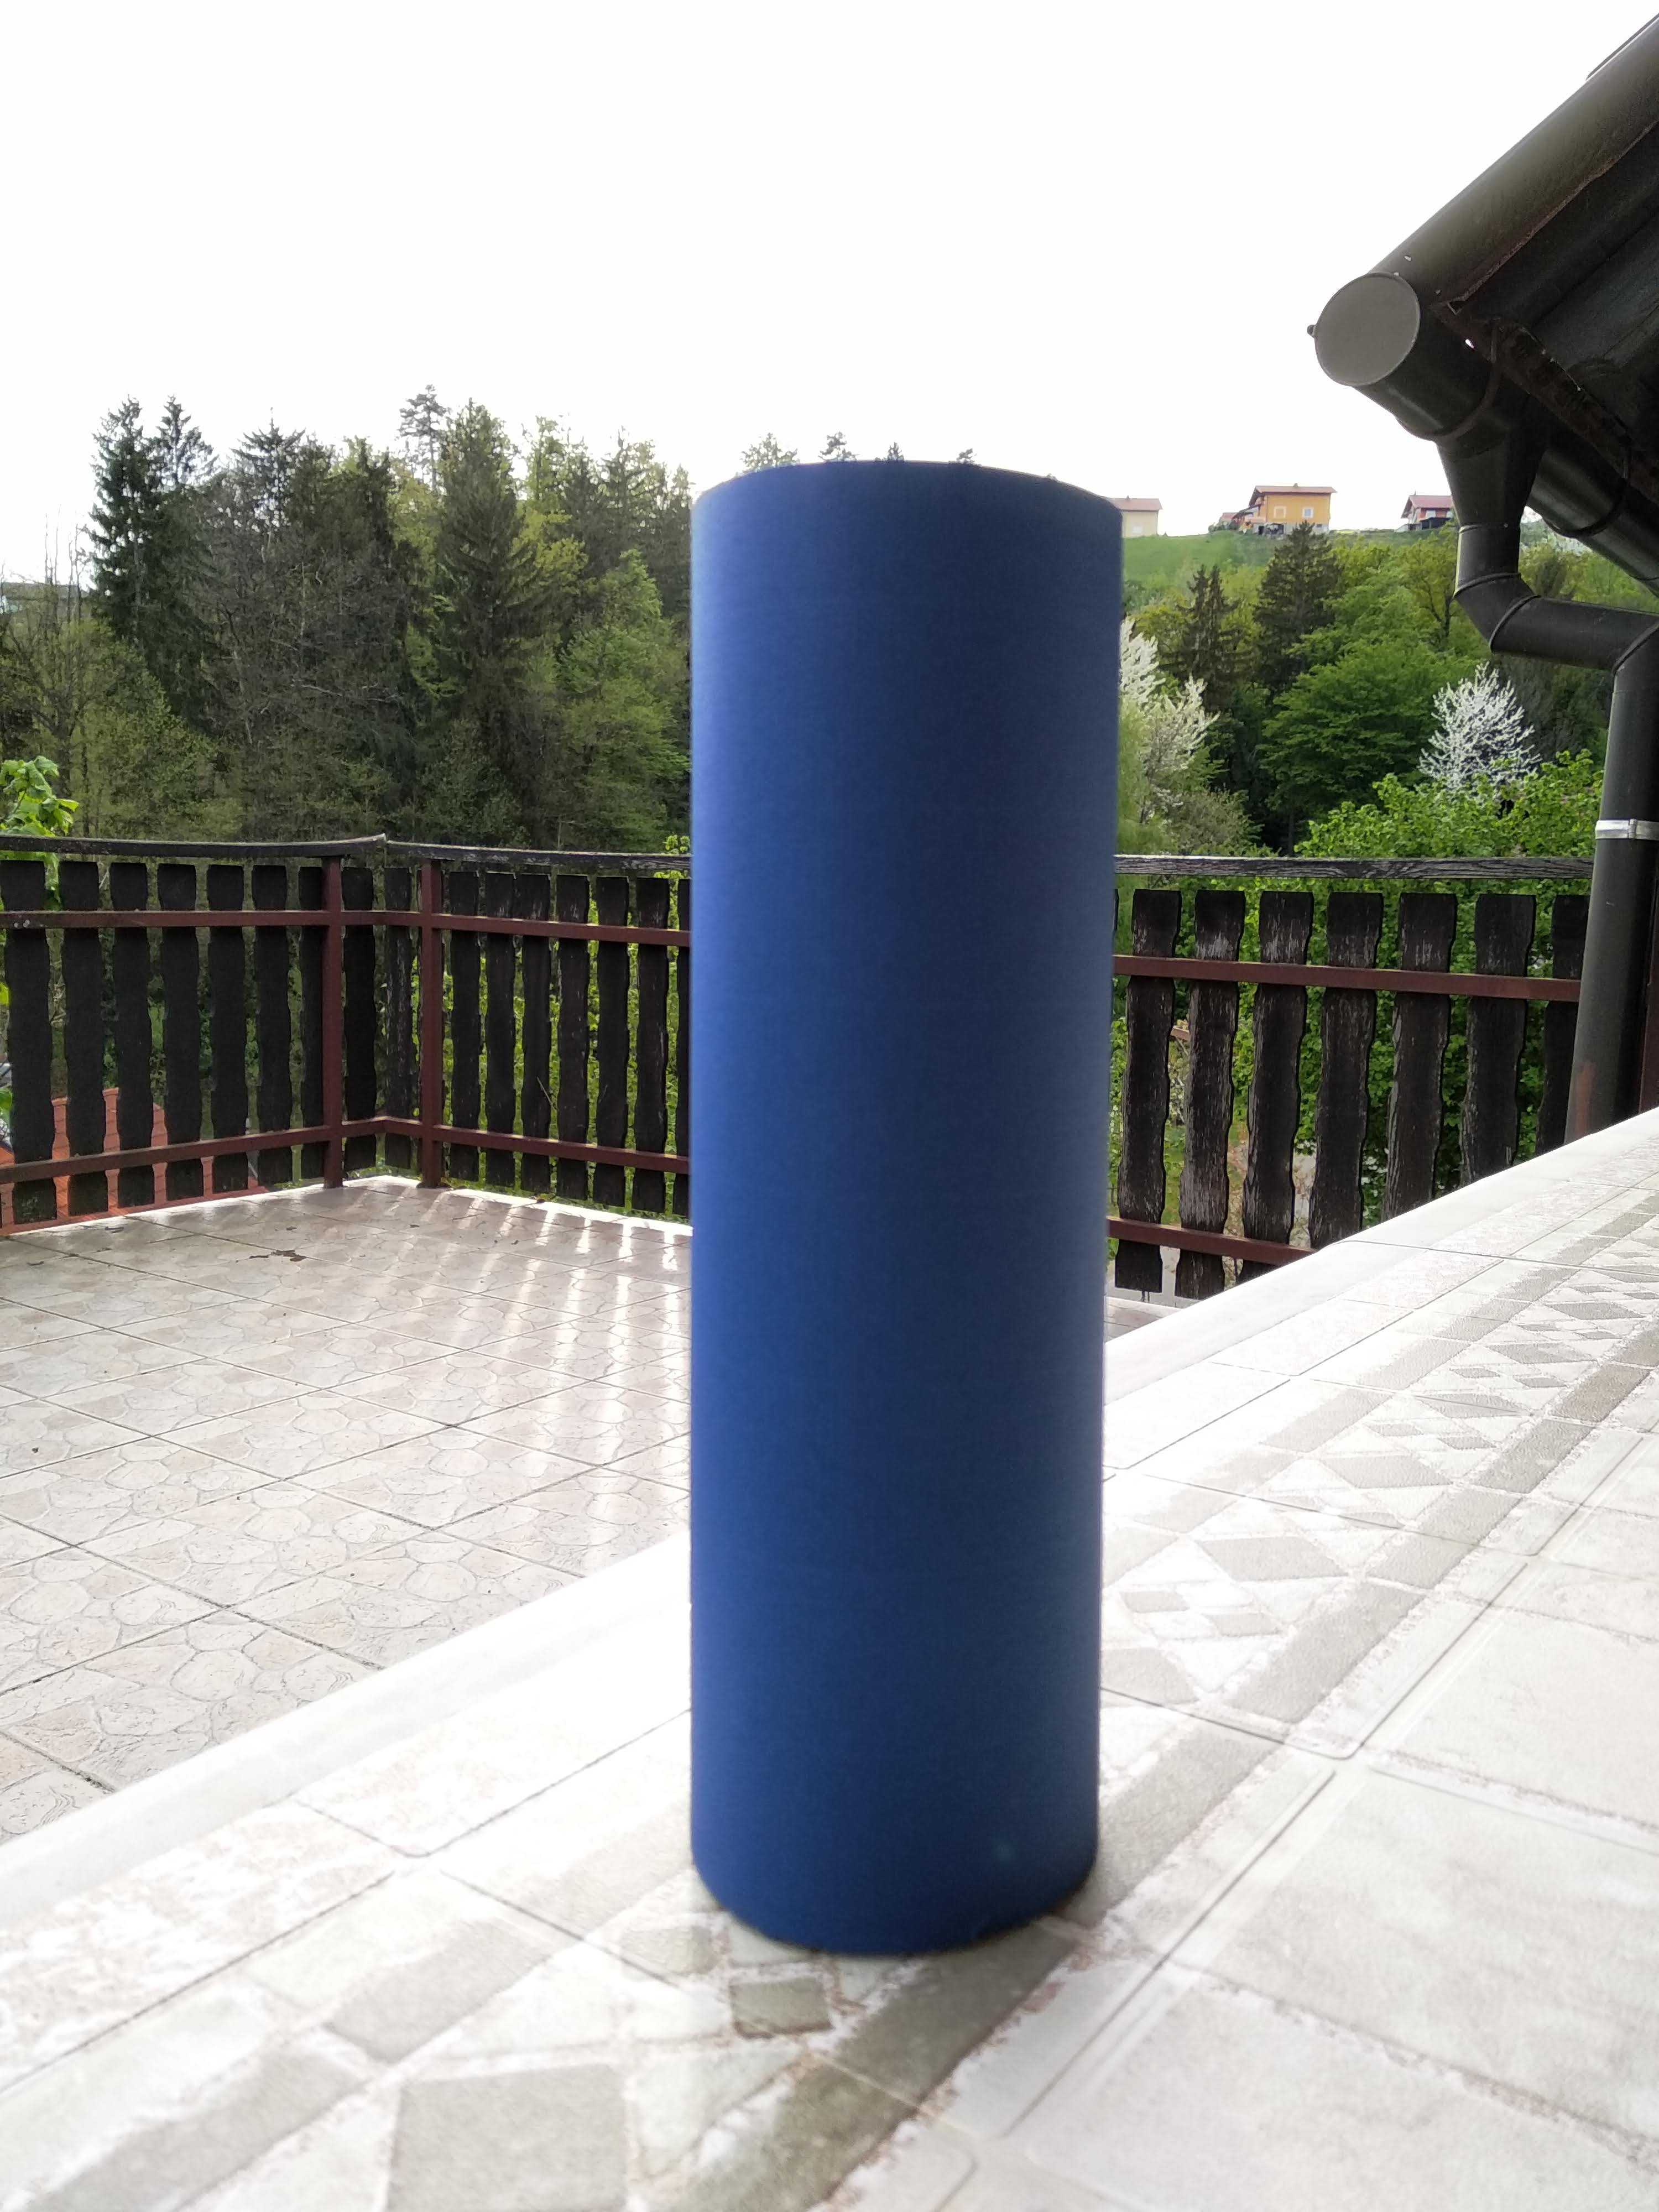
\includegraphics[width=.13\linewidth]{images/test04.jpg}
		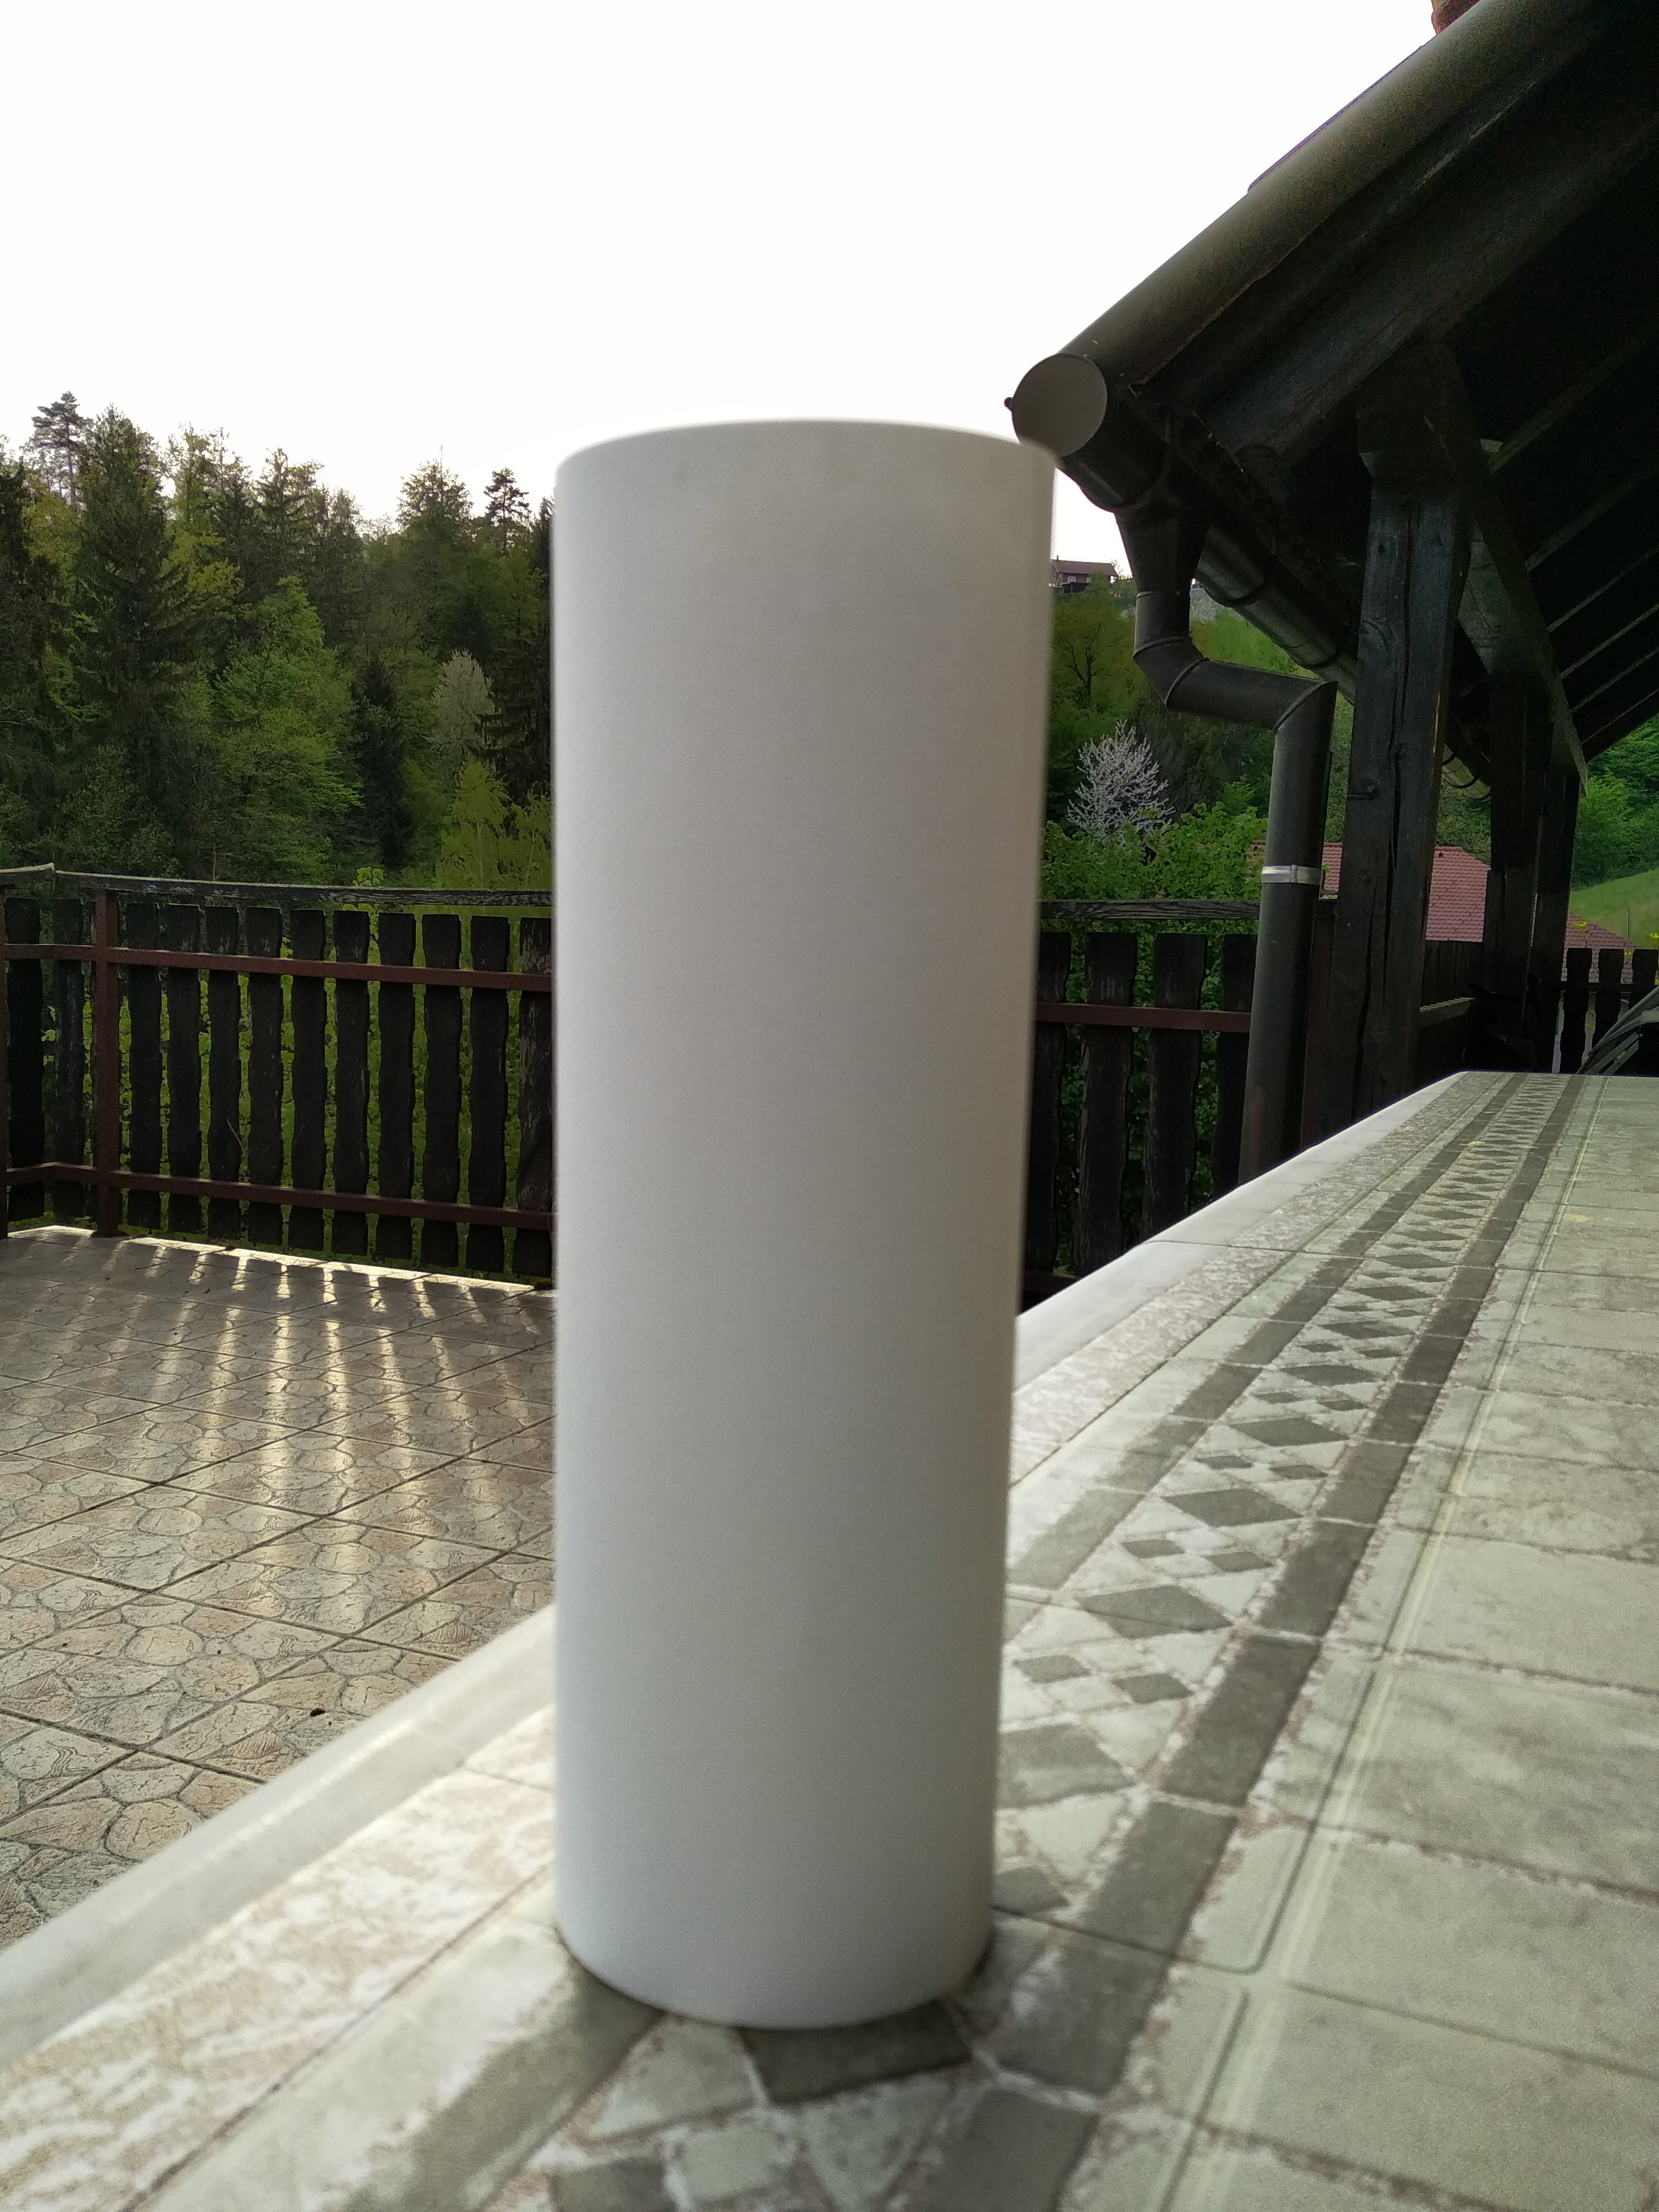
\includegraphics[width=.13\linewidth]{images/test05.jpg}
		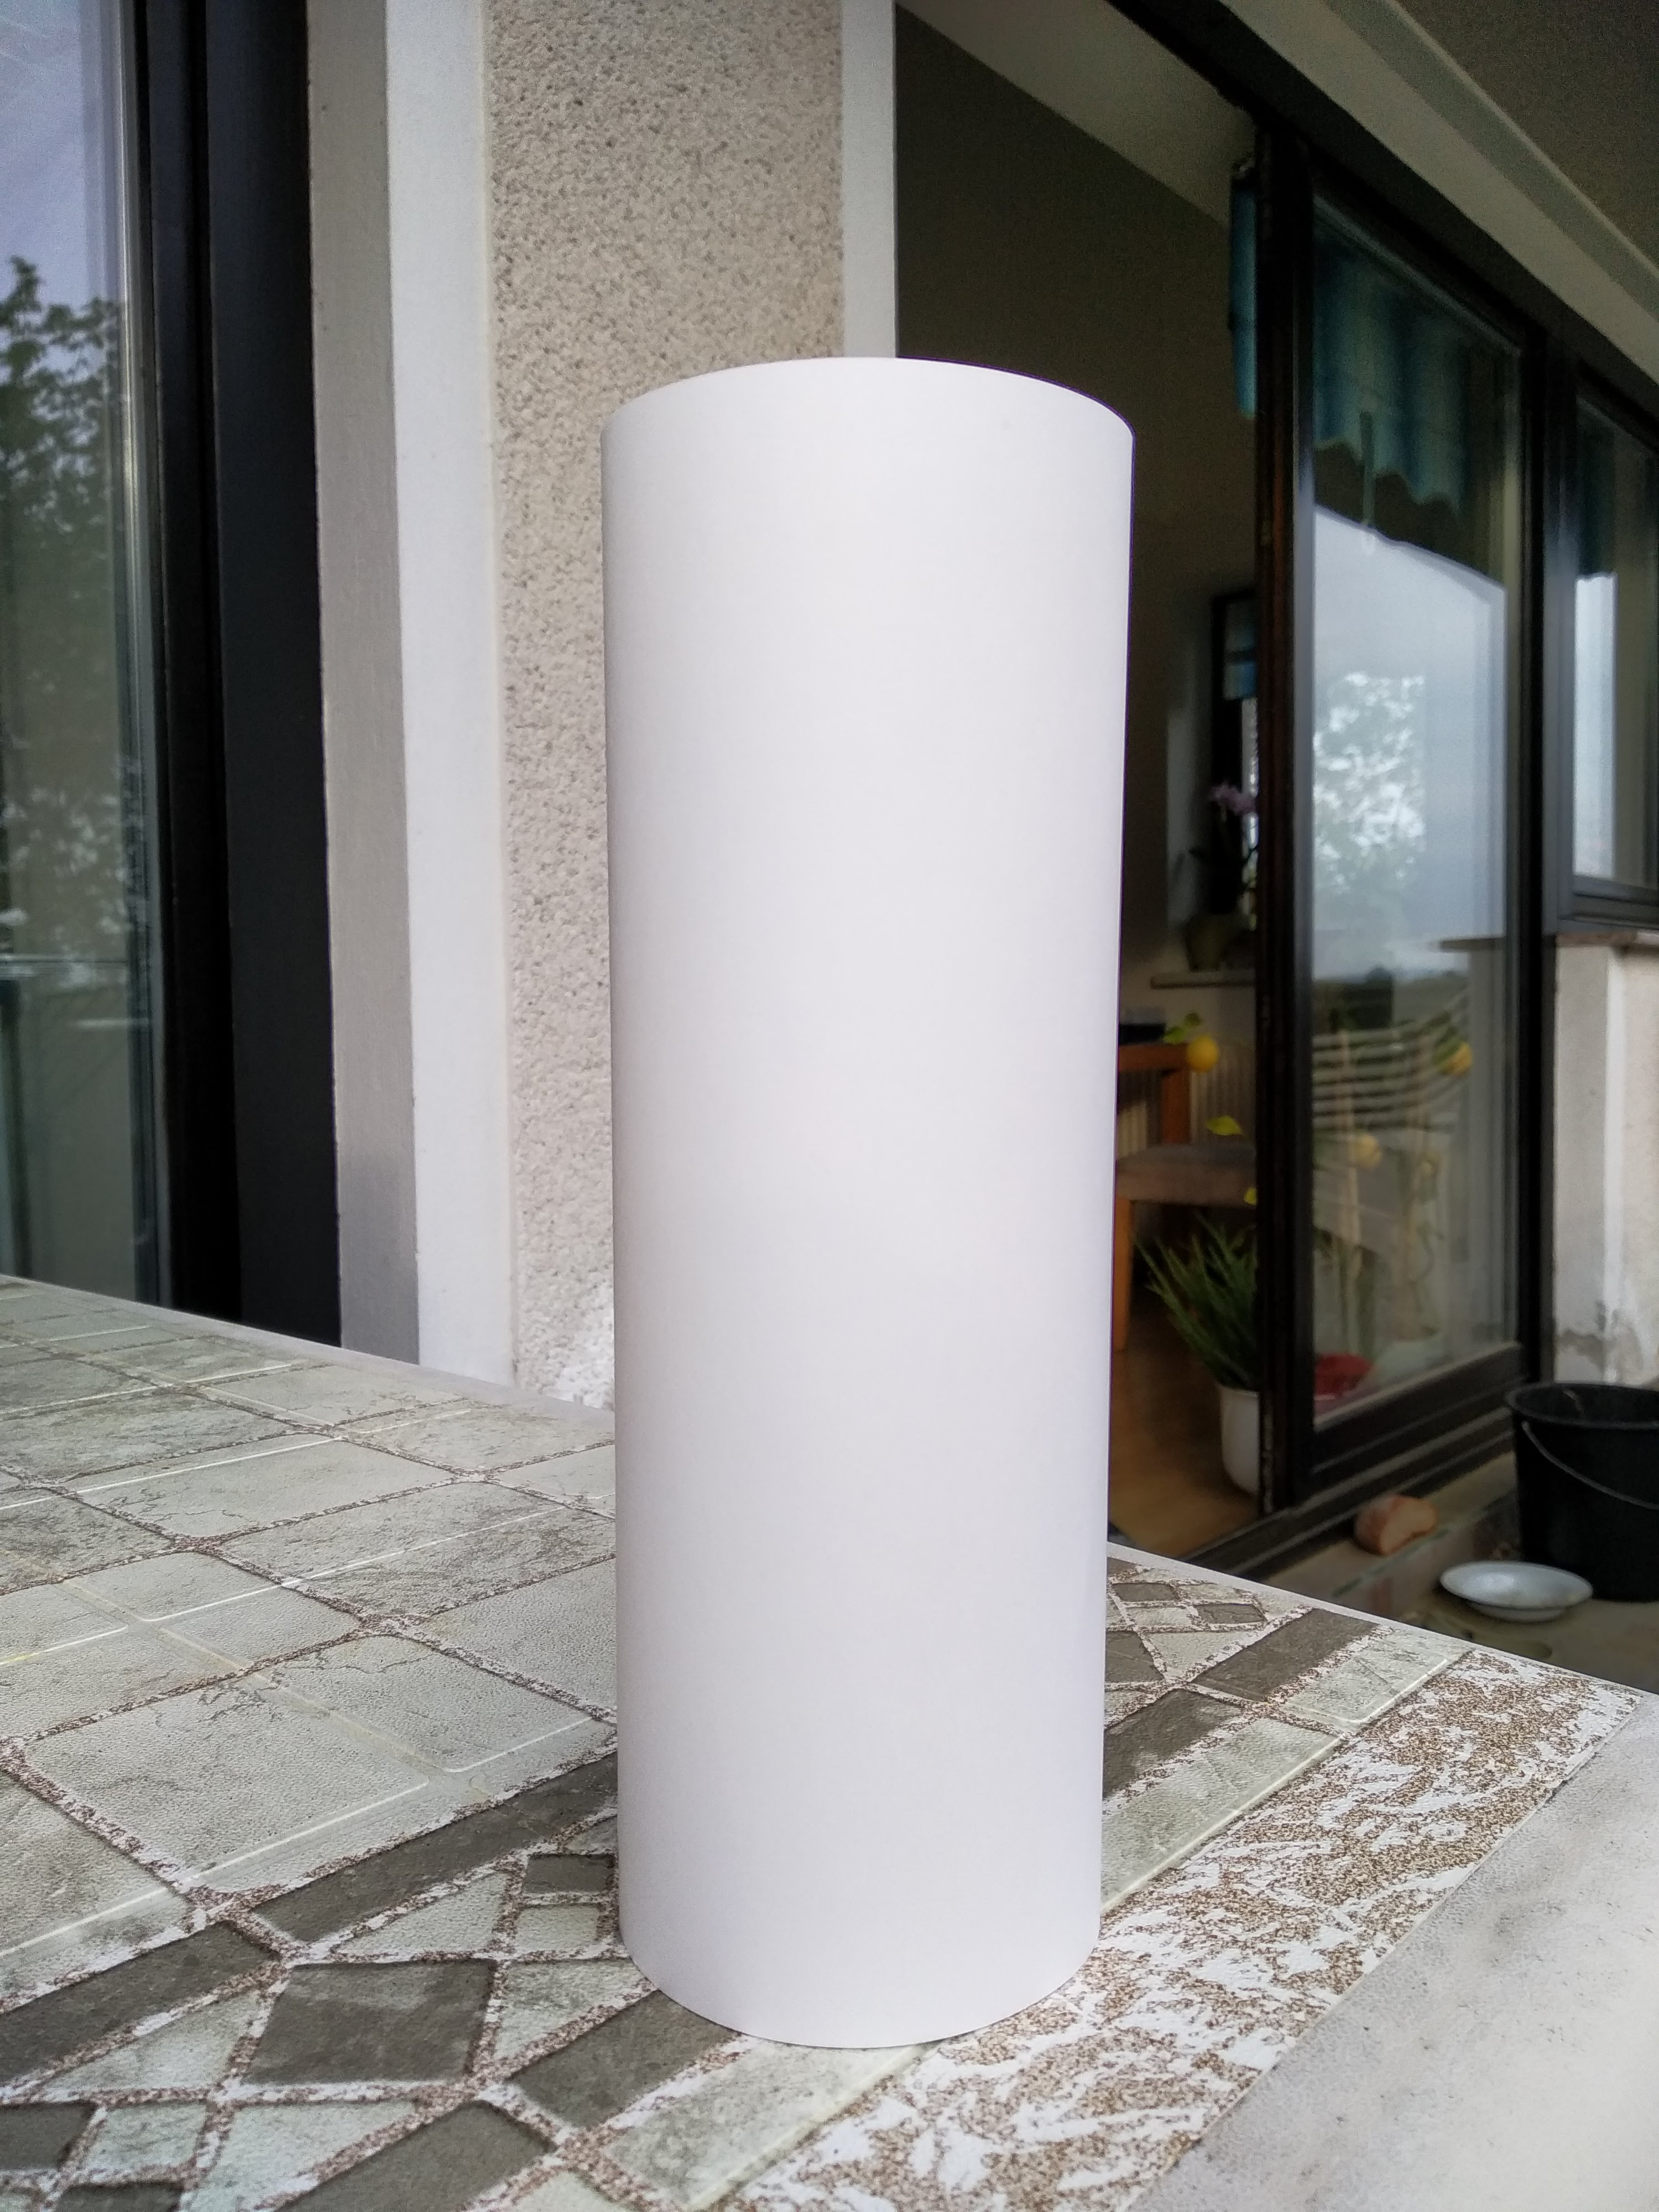
\includegraphics[width=.13\linewidth]{images/test06.jpg} \\
		\vspace{3pt}
		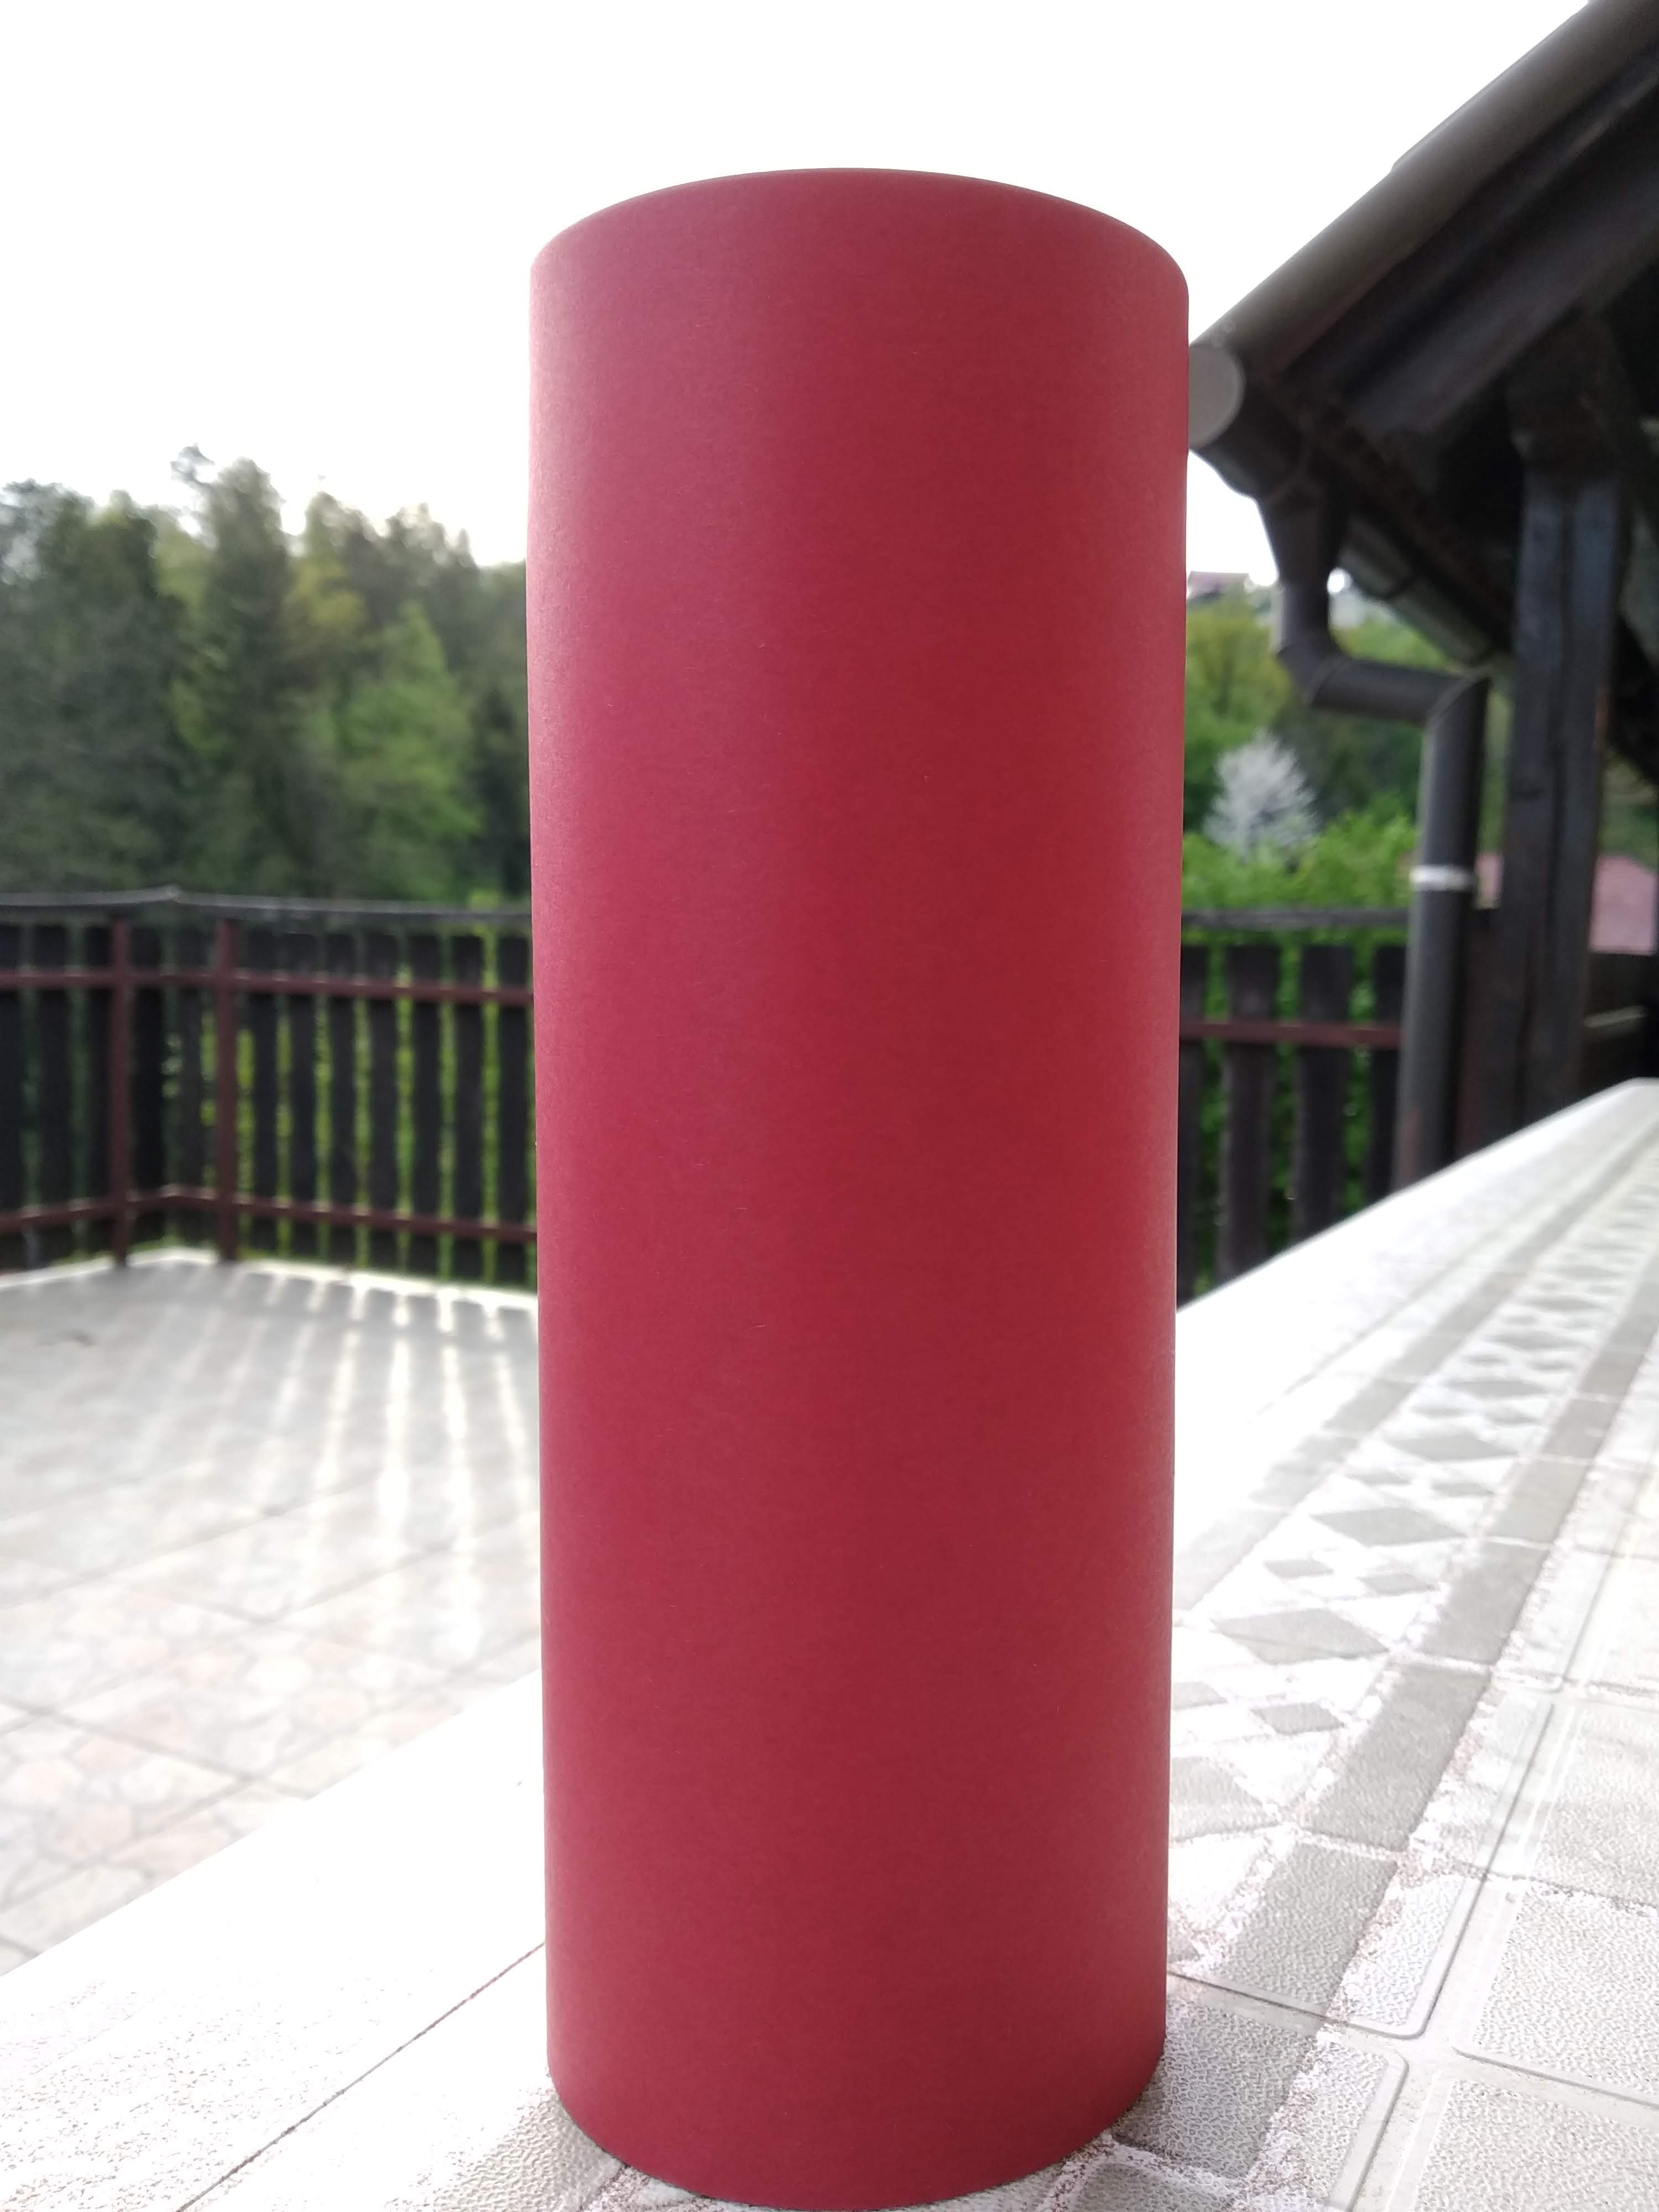
\includegraphics[width=.13\linewidth]{images/test07.jpg}
		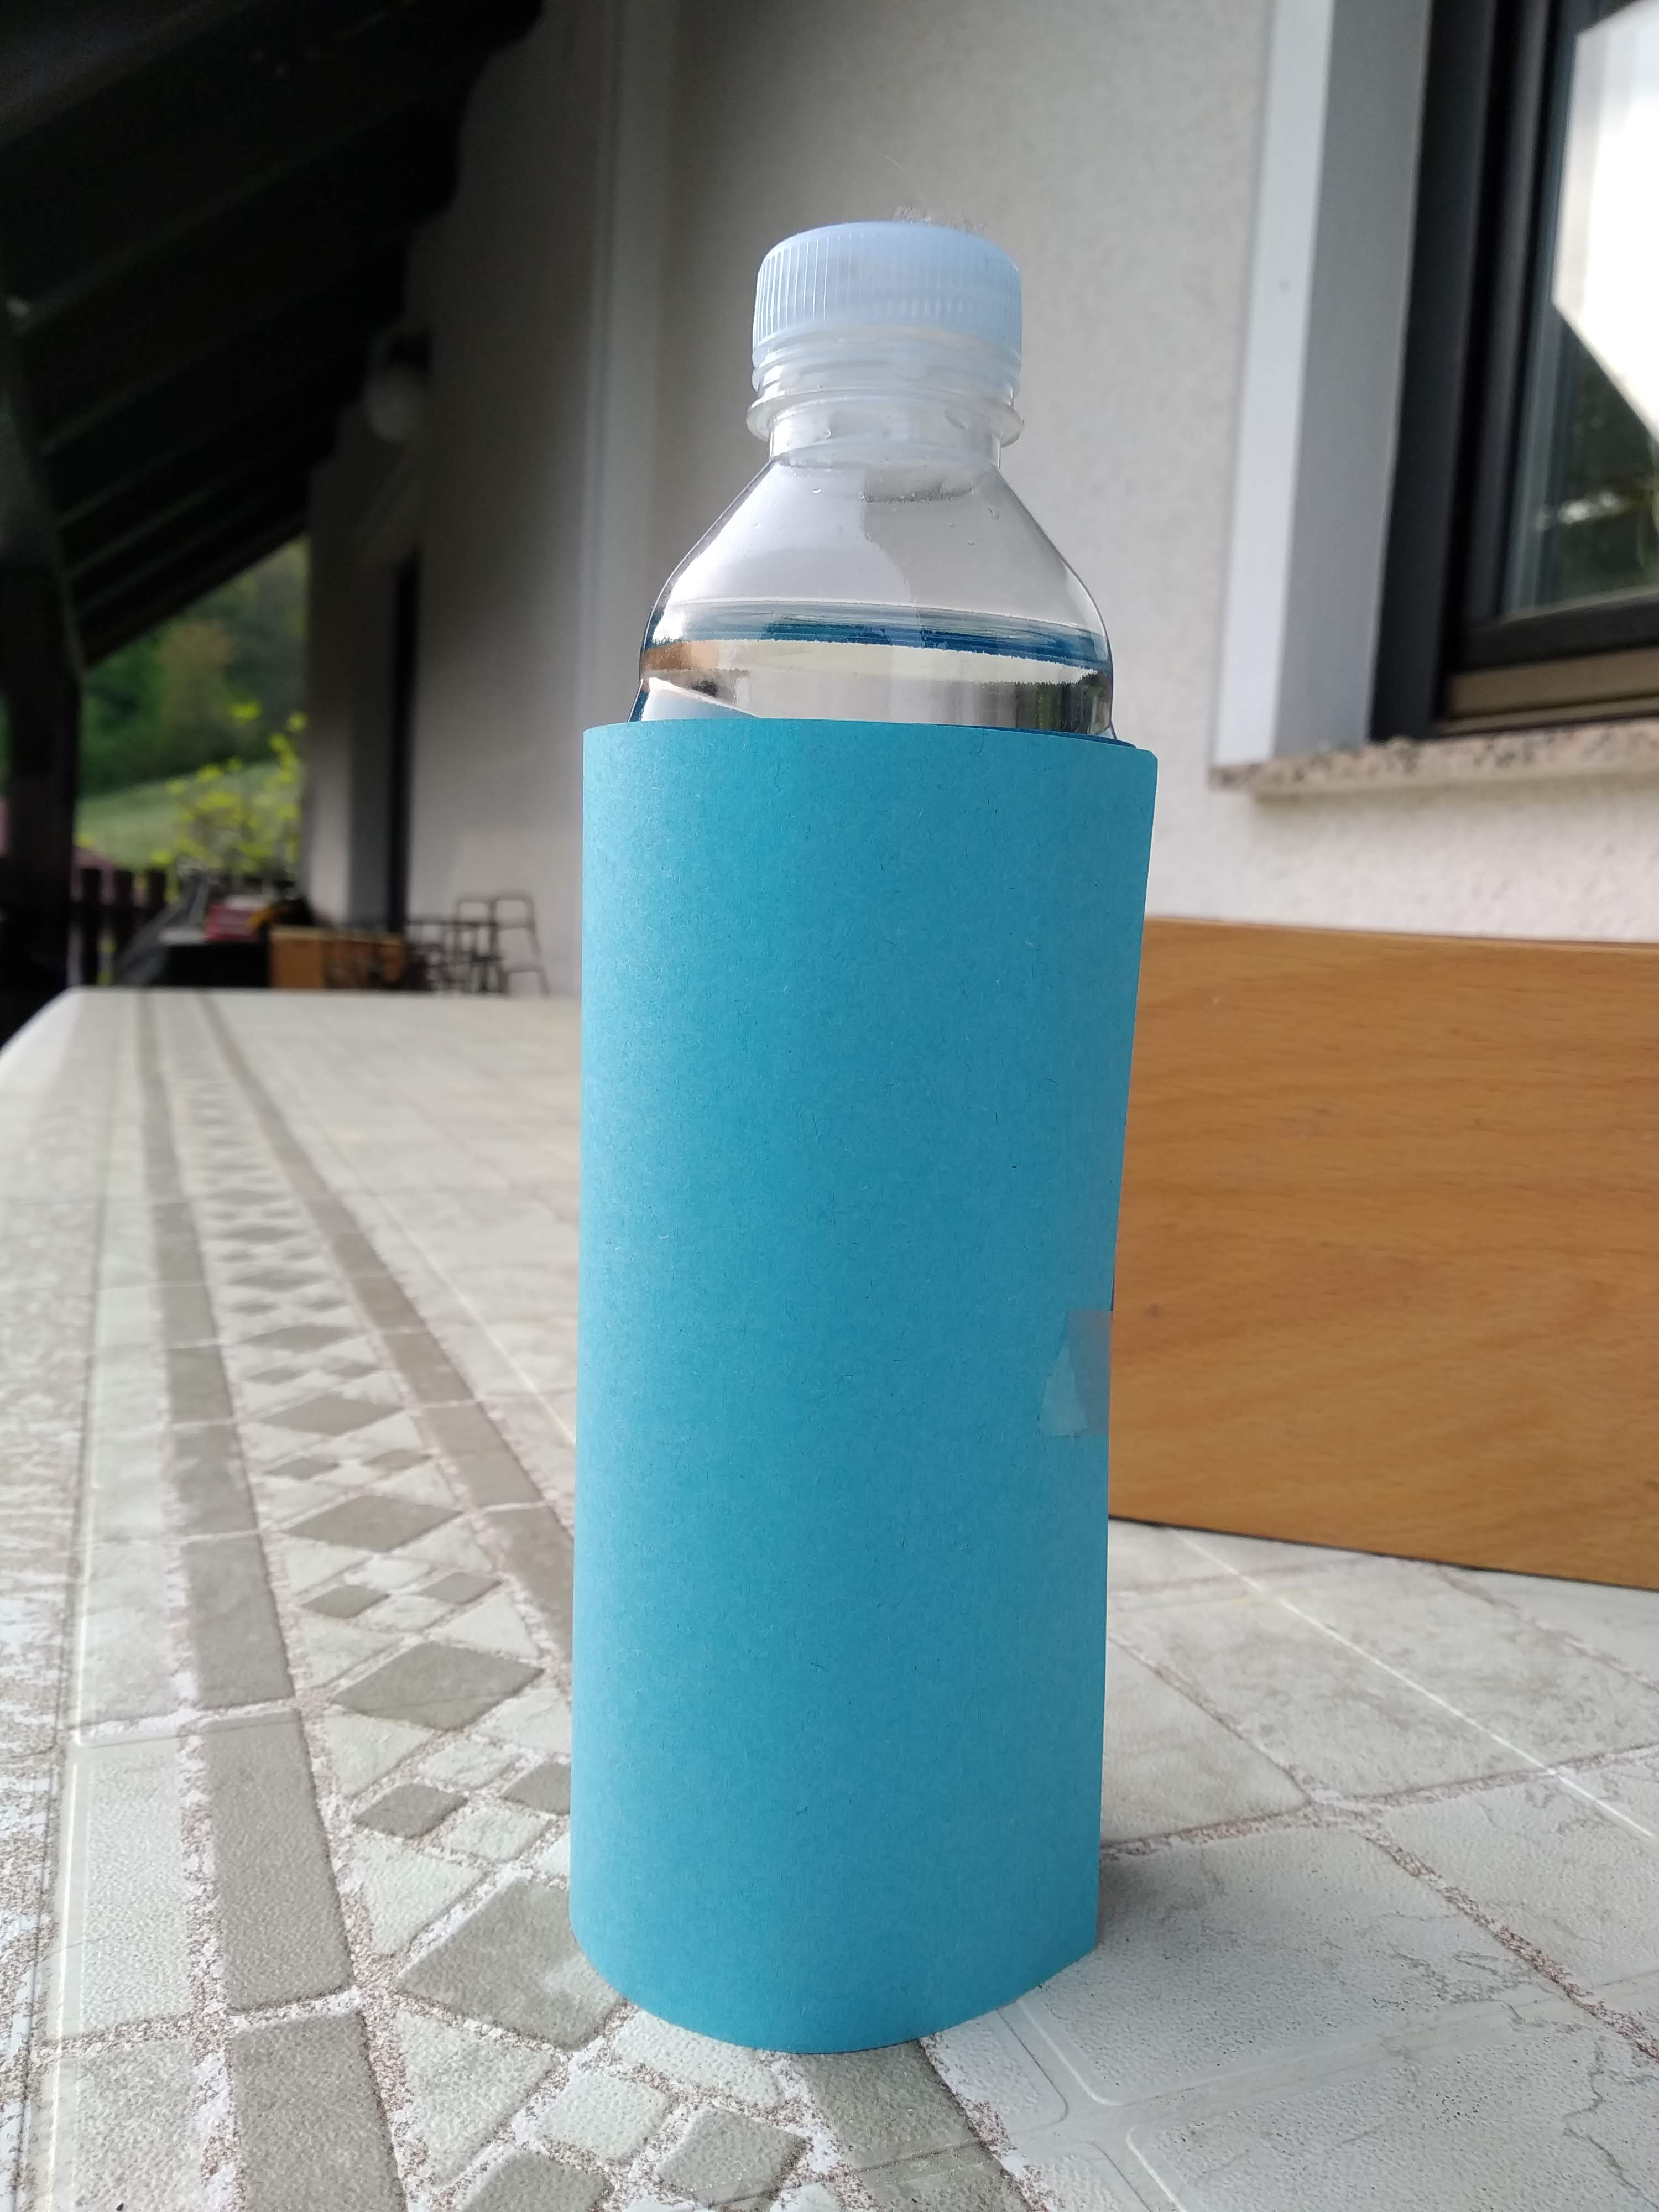
\includegraphics[width=.13\linewidth]{images/test08.jpg}
		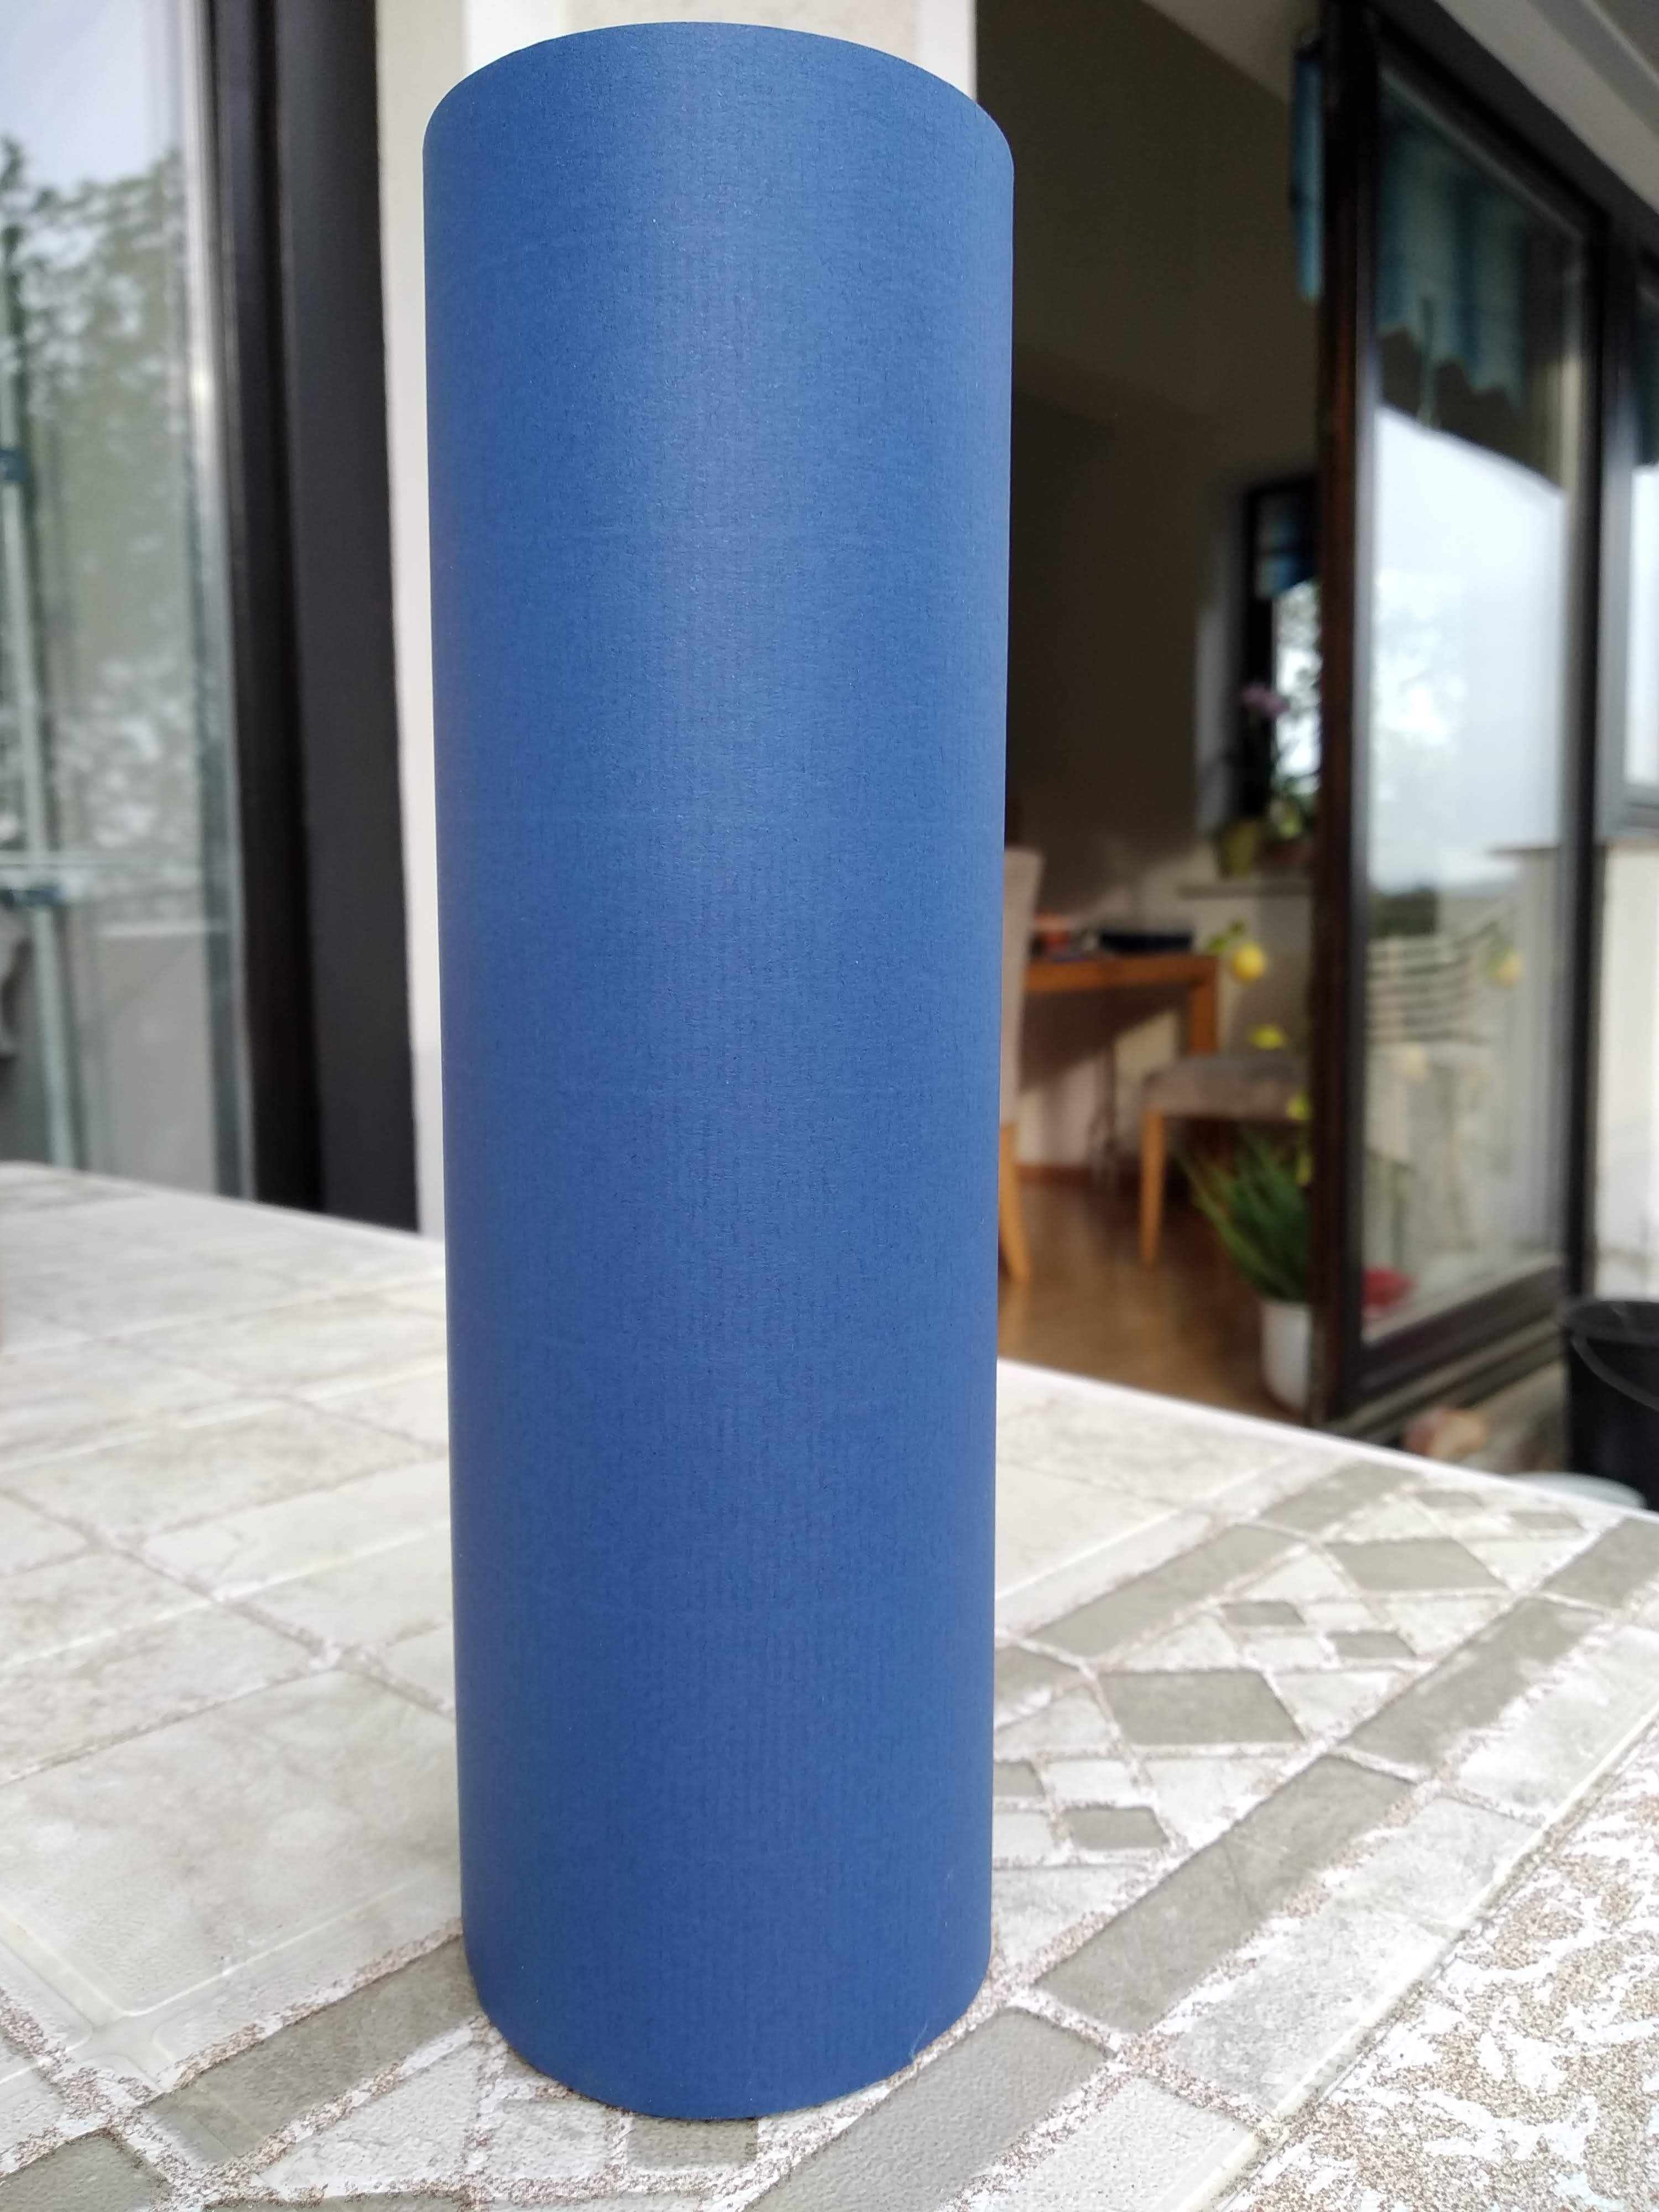
\includegraphics[width=.13\linewidth]{images/test_09_remove_if_too_many_photos.jpg}
		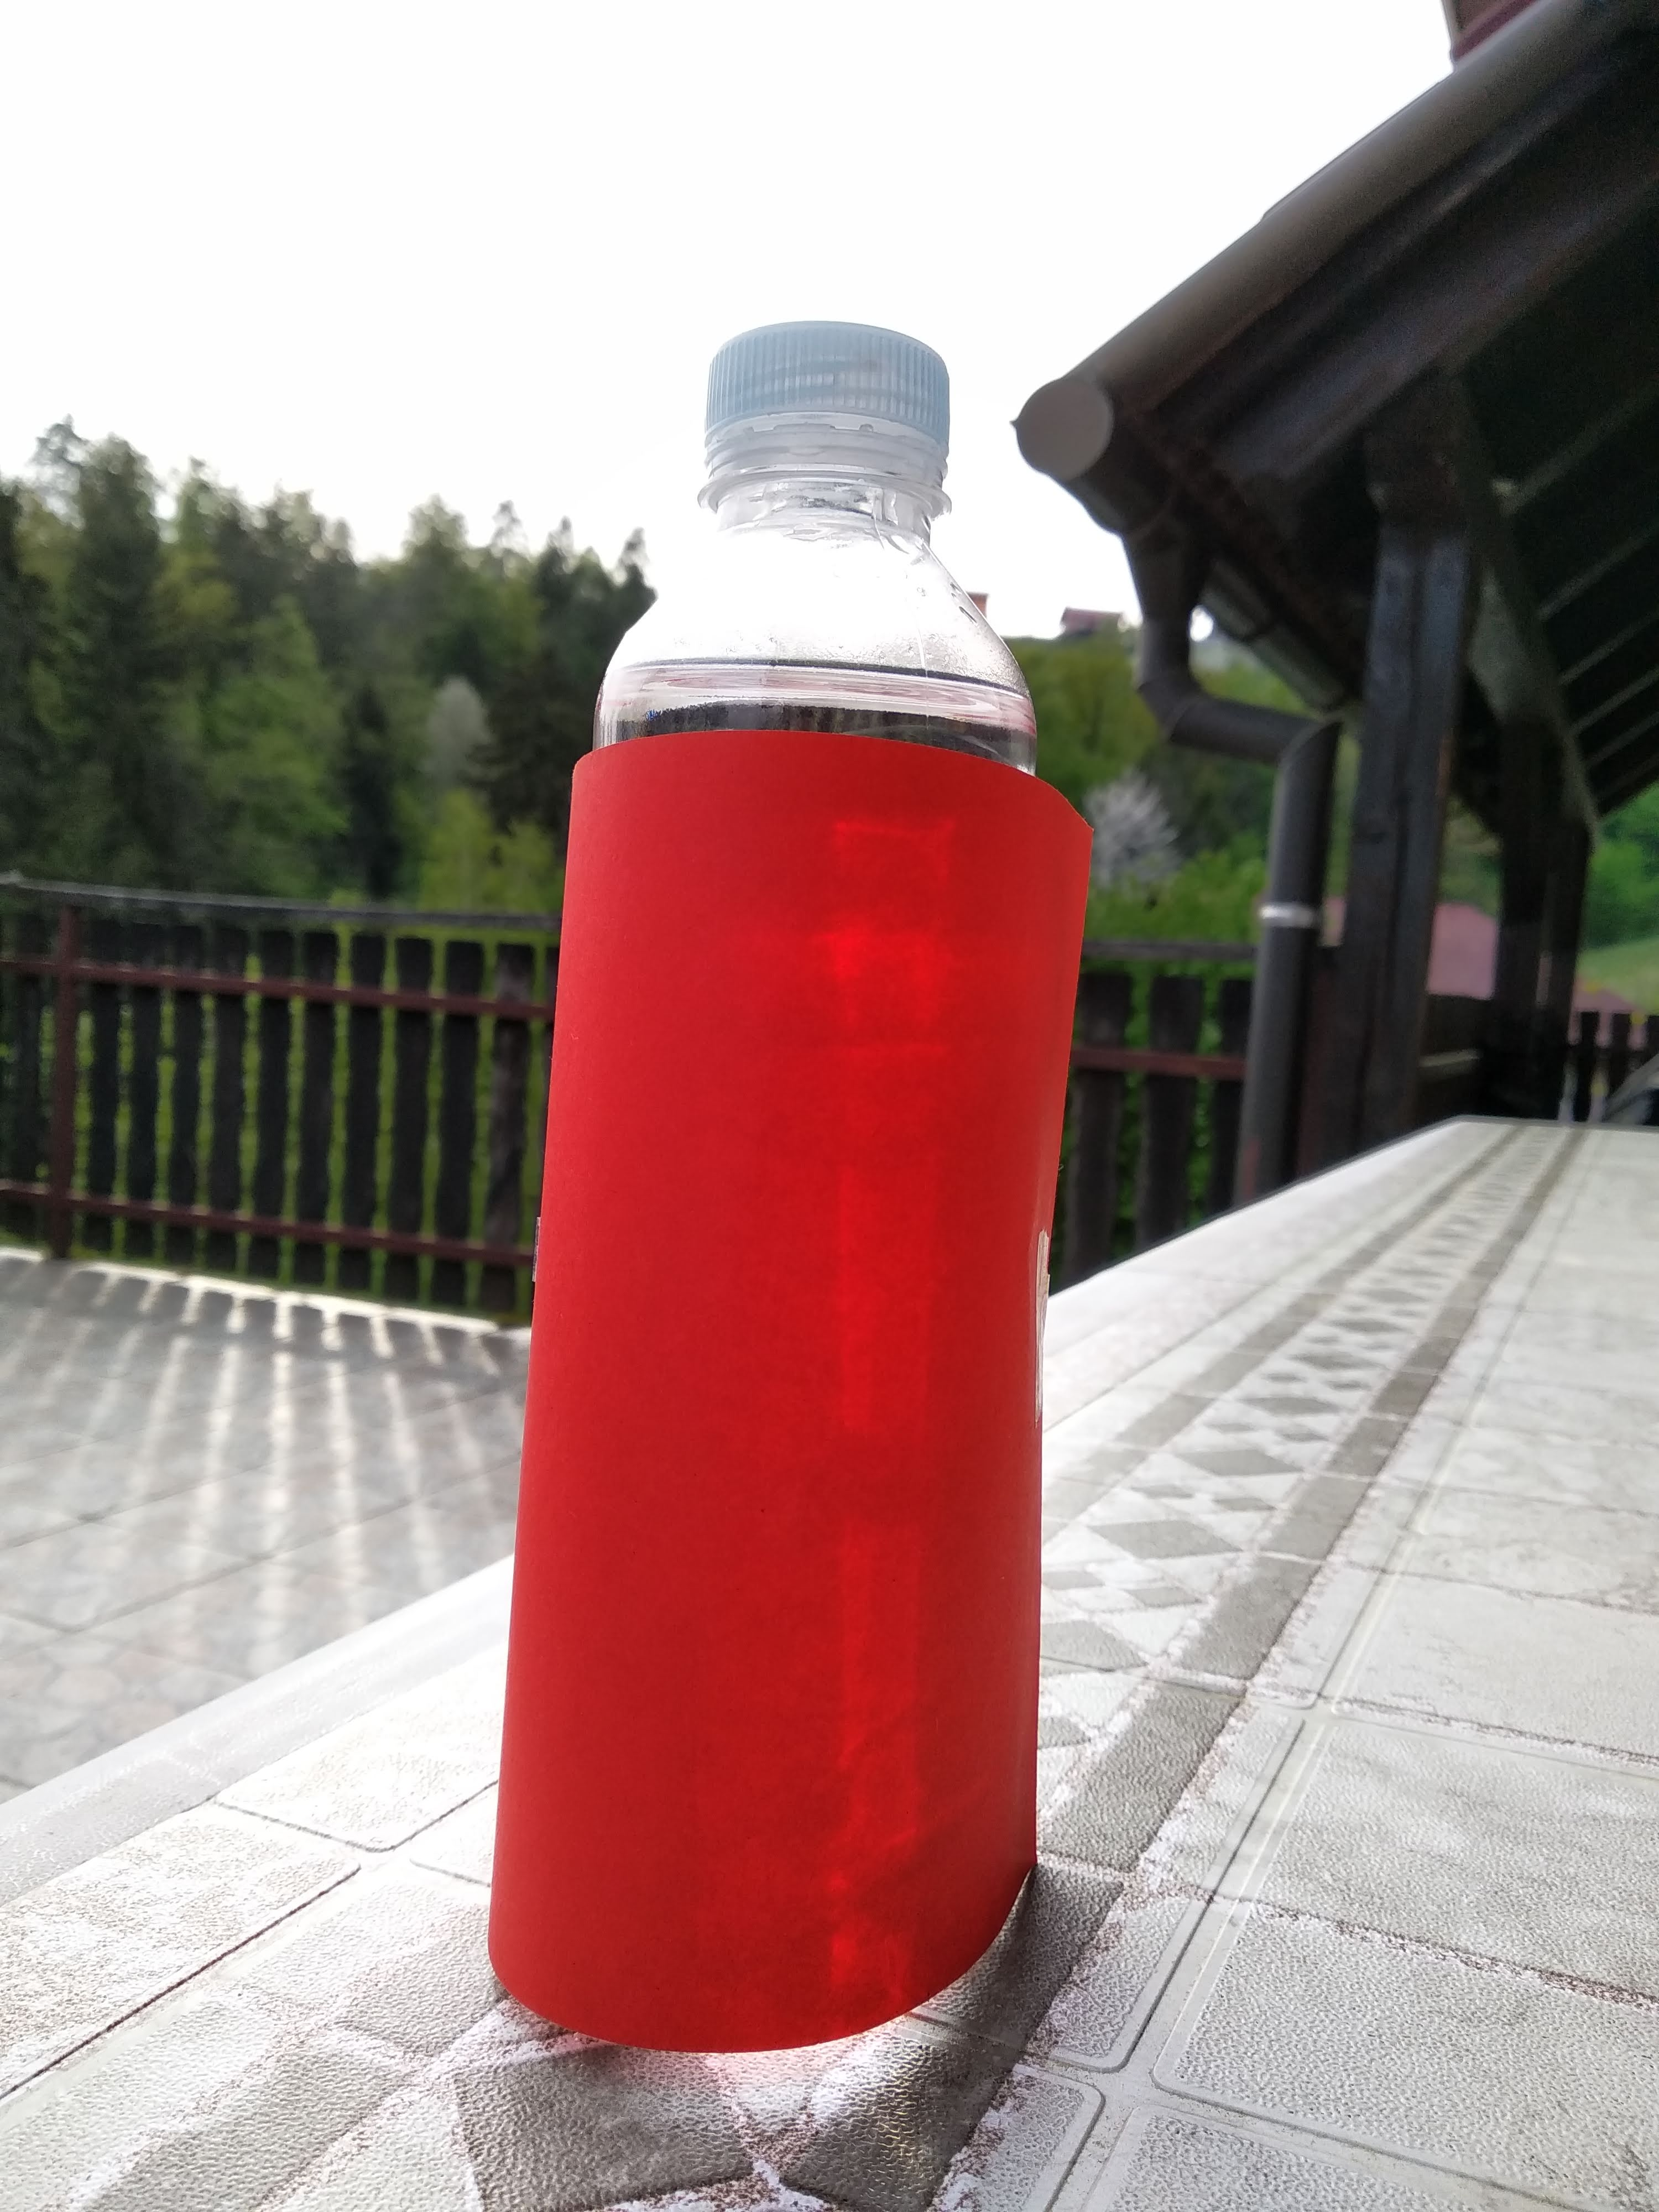
\includegraphics[width=.13\linewidth]{images/test_10_remove_if_too_many_photos.jpg}
		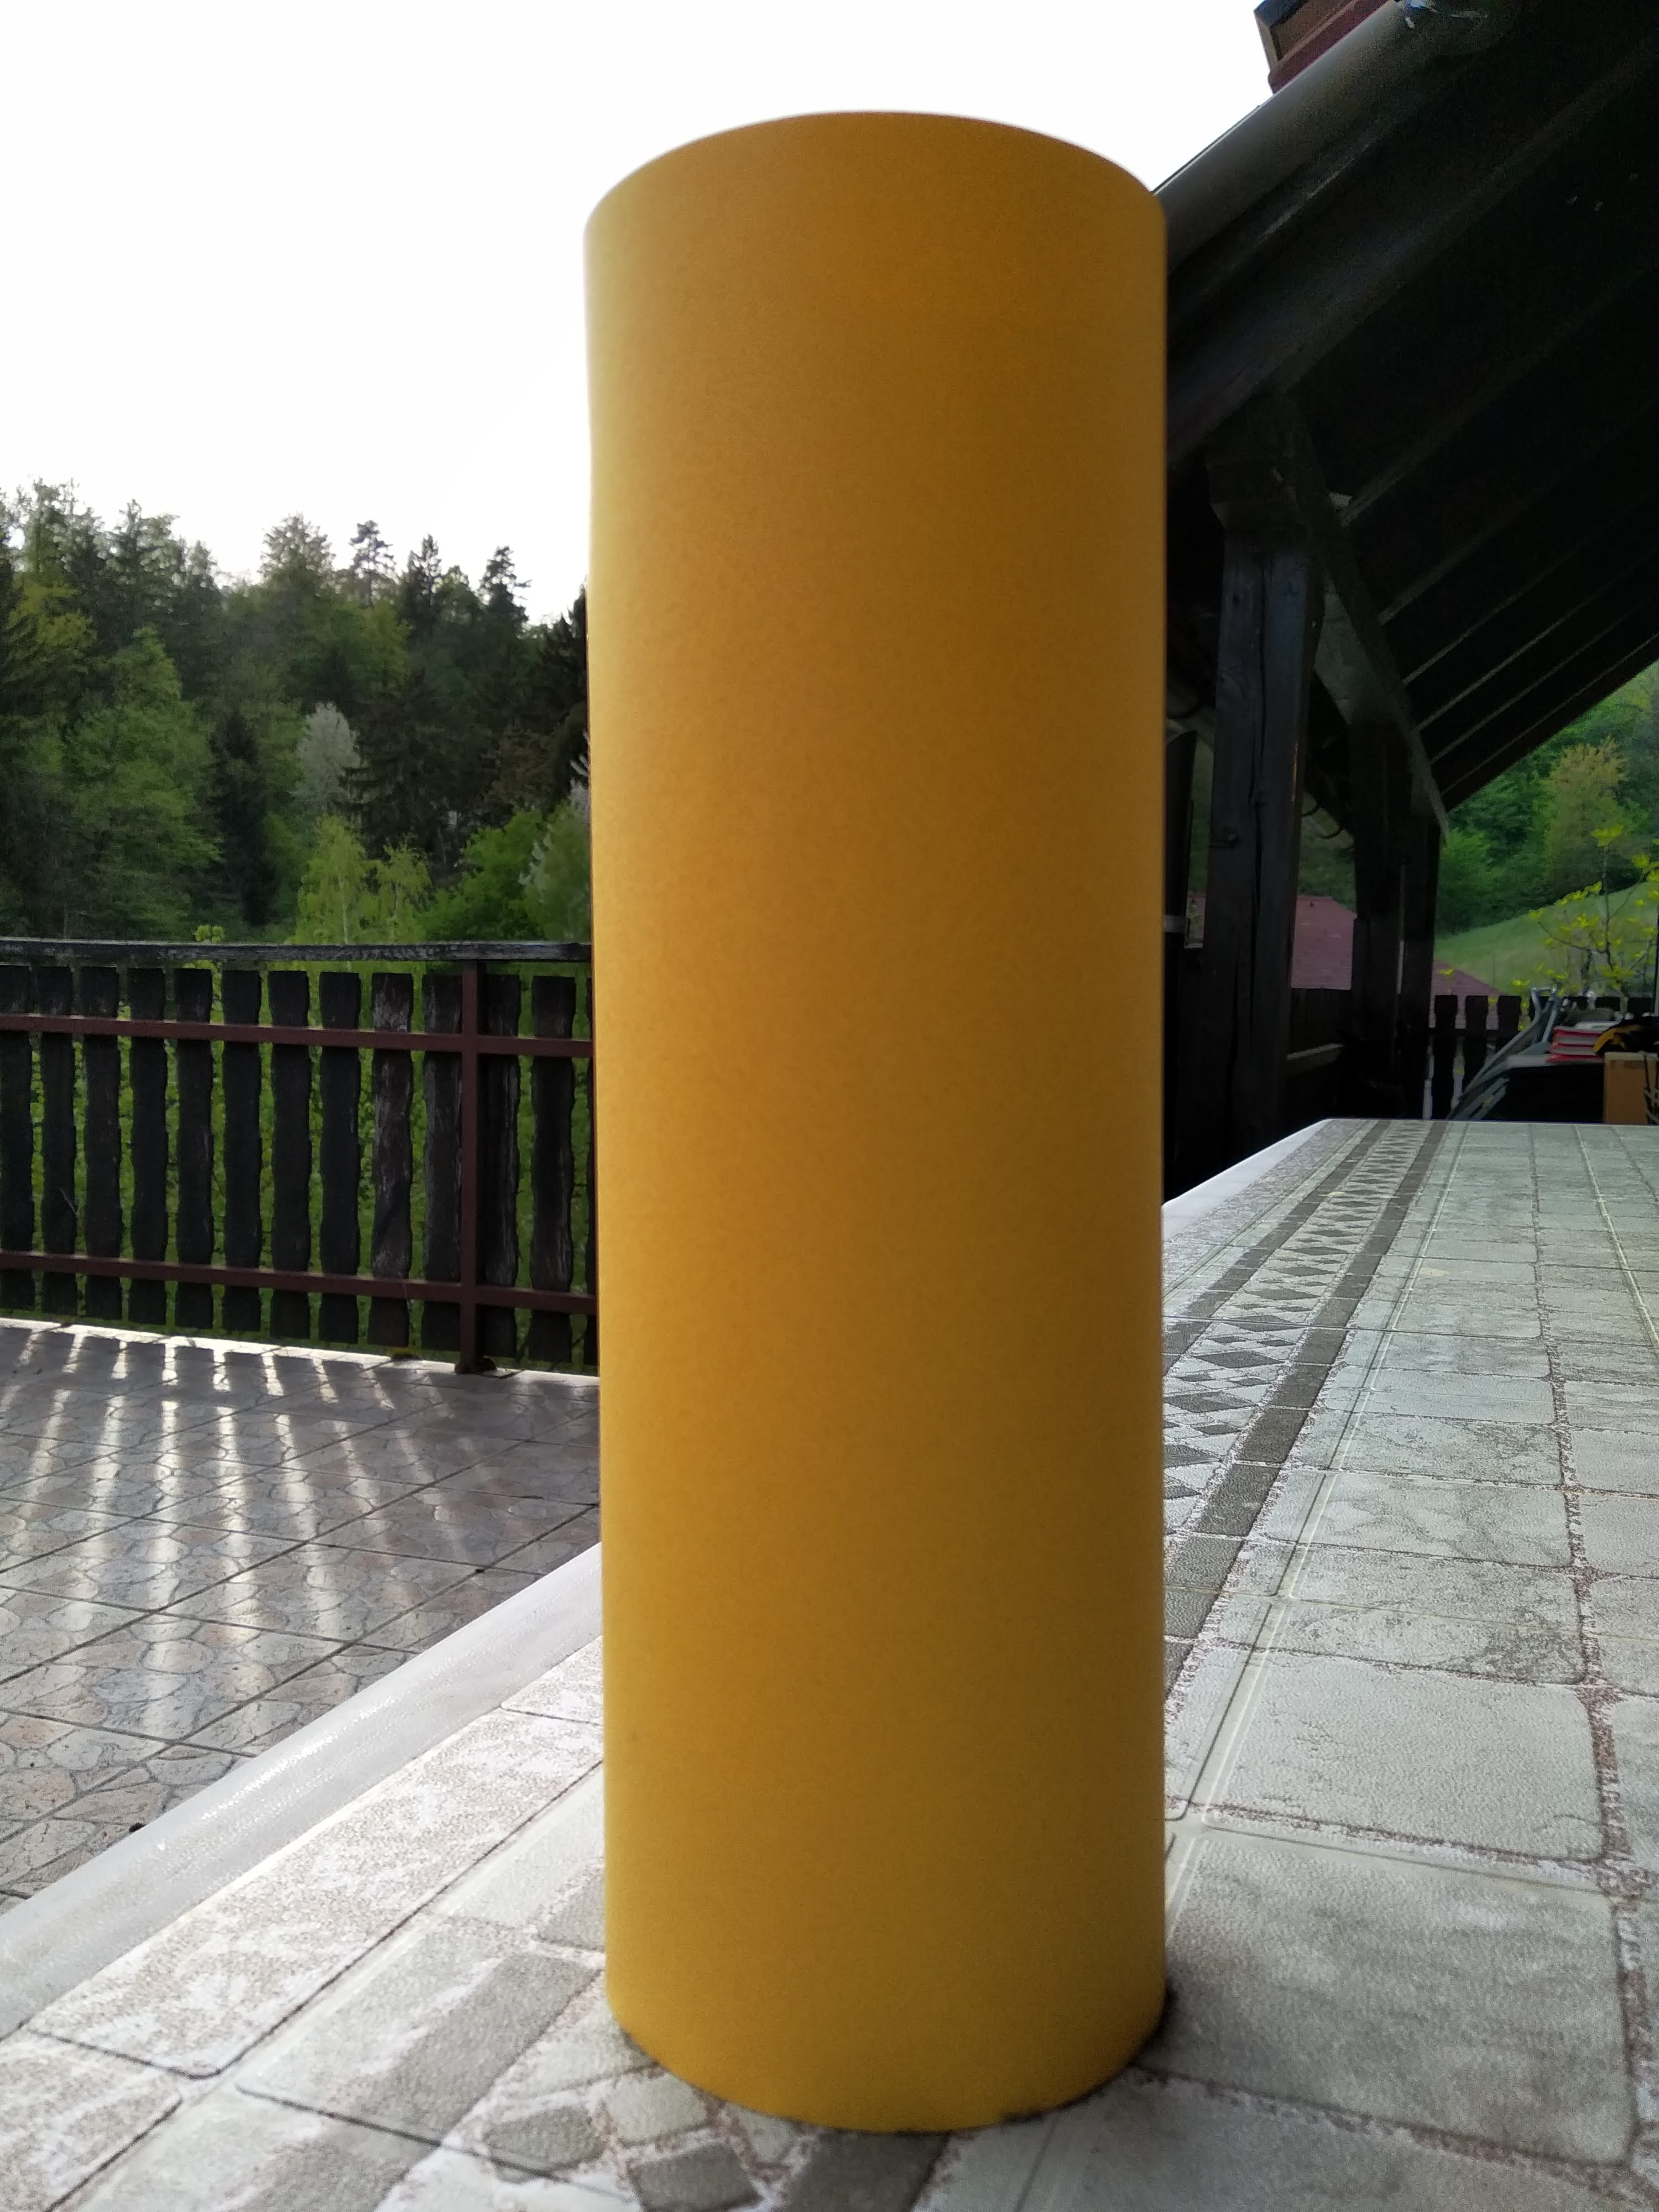
\includegraphics[width=.13\linewidth]{images/test_11_remove_if_too_many_photos.jpg}
		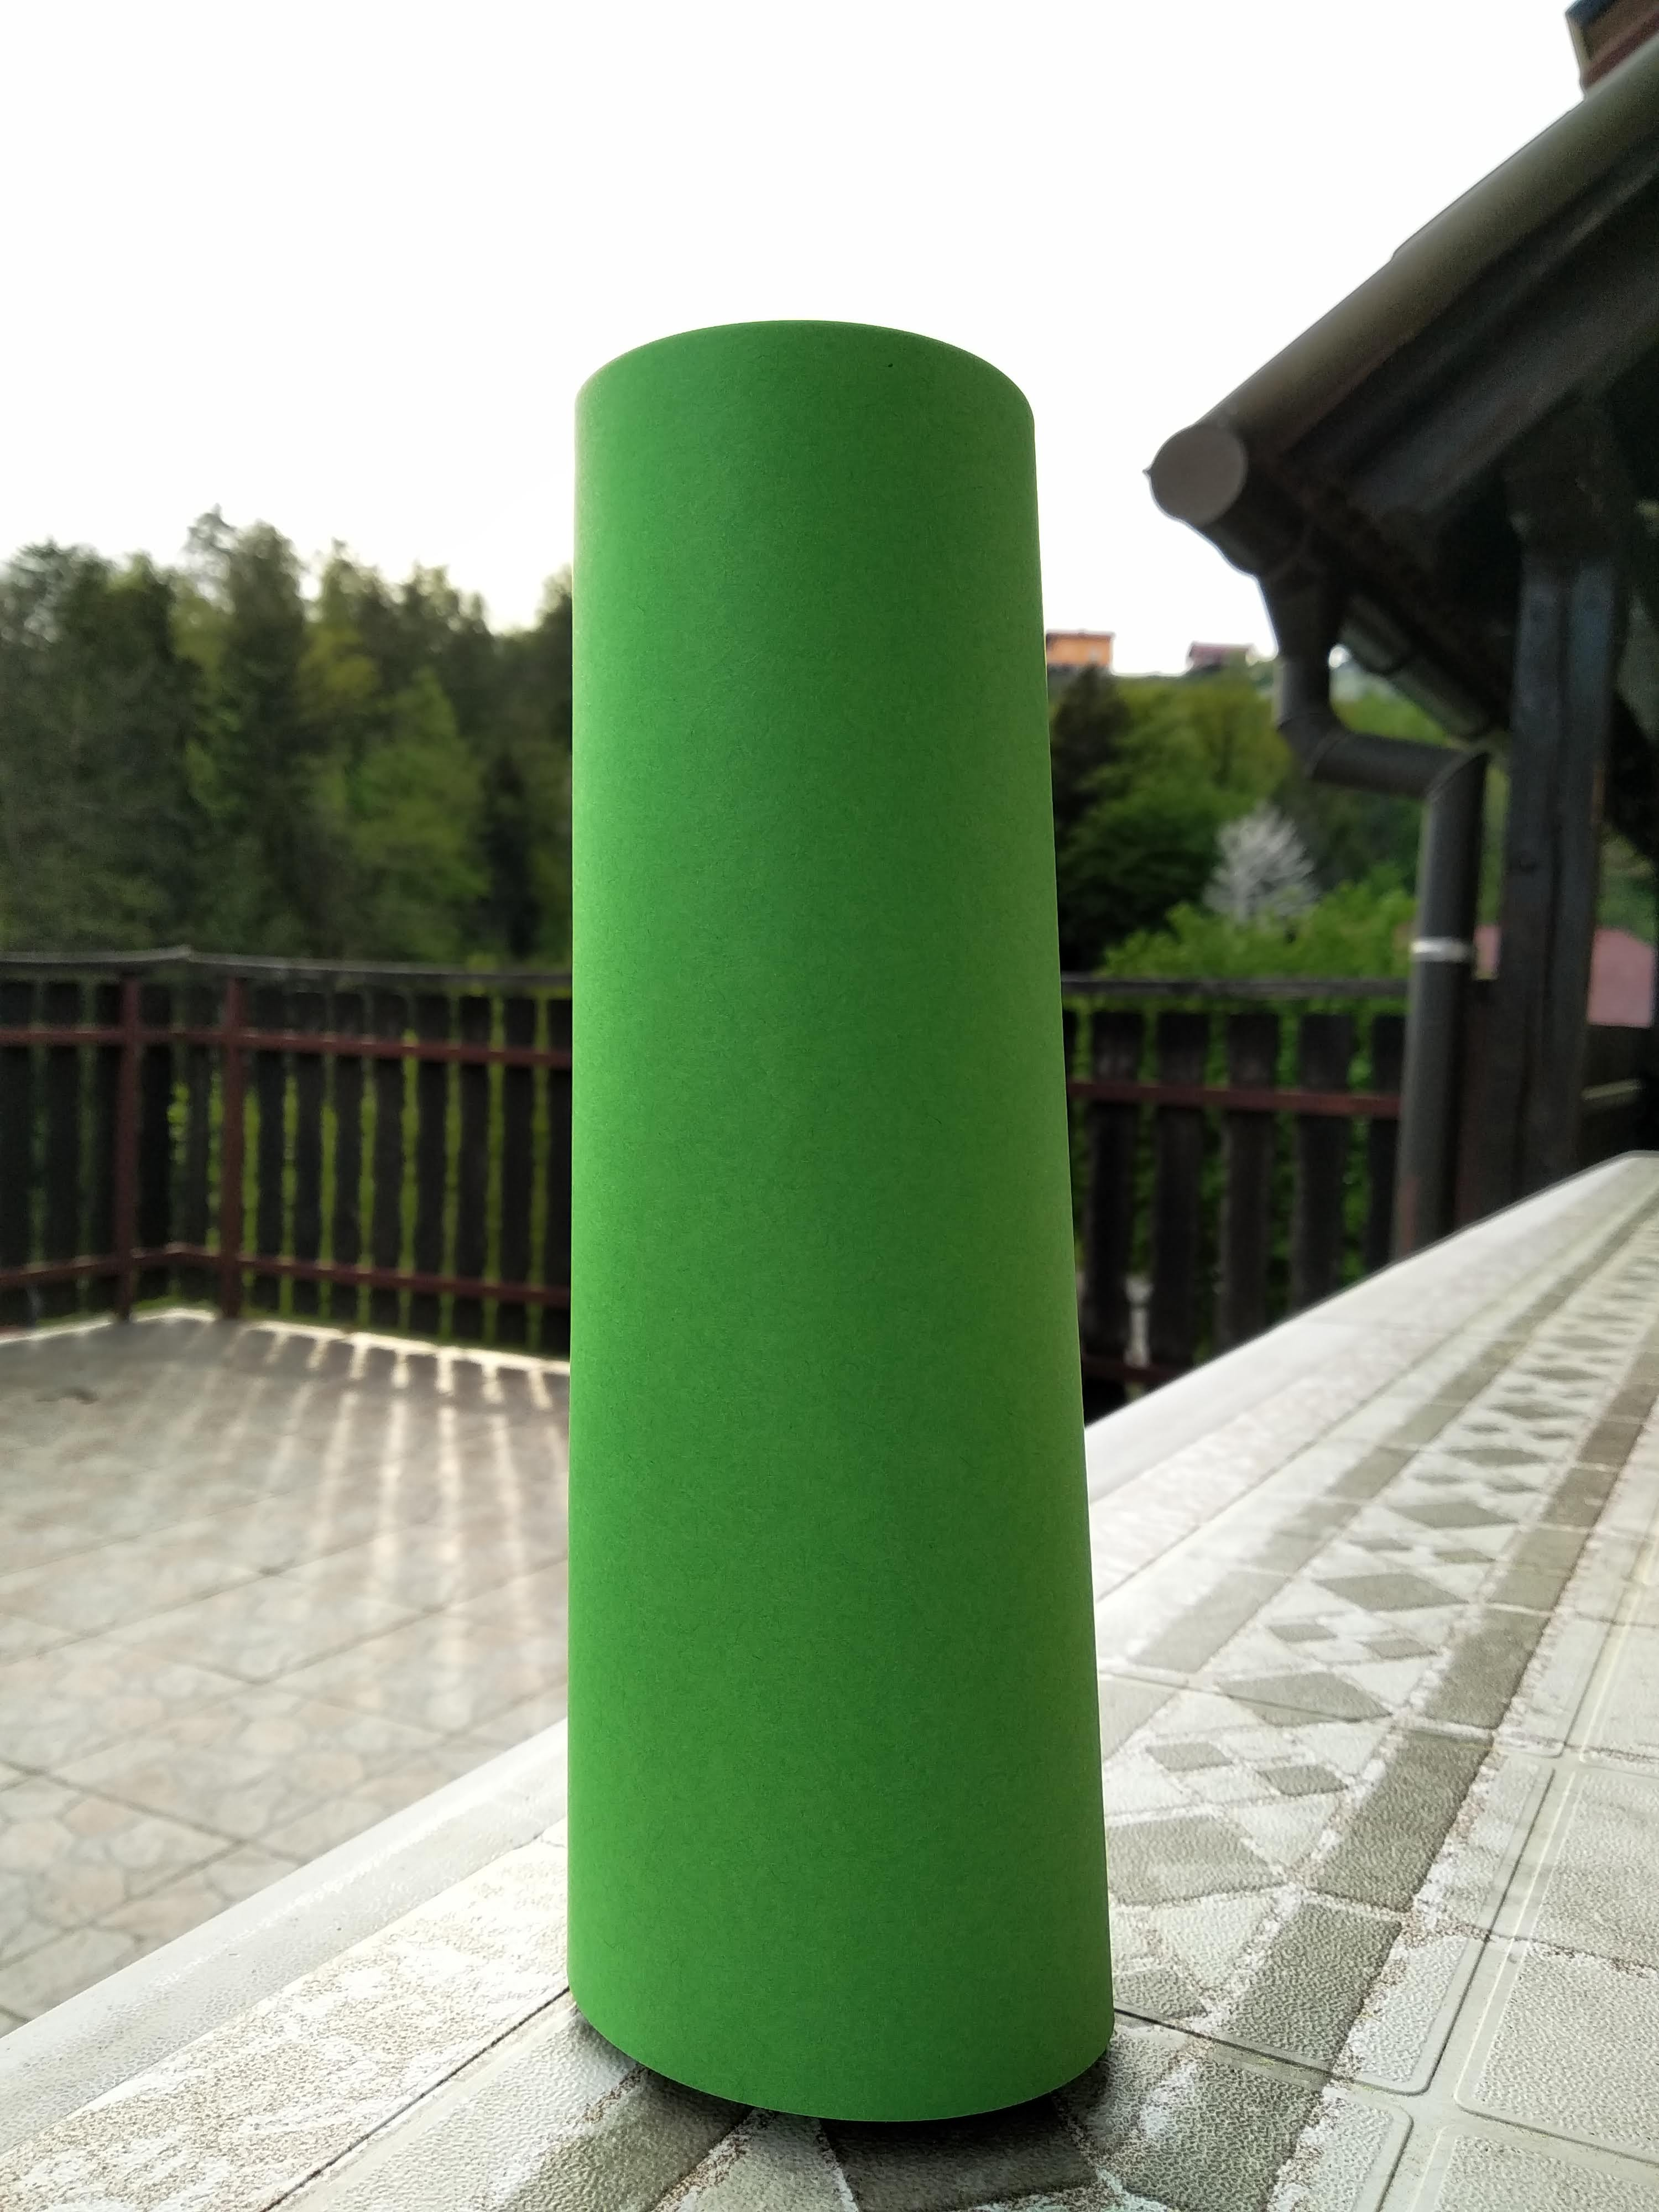
\includegraphics[width=.13\linewidth]{images/test_12_remove_if_too_many_photos.jpg}
		\caption{Testing set}
	\end{figure}

	Just as the training images, these were cropped and shrinked befor they were fed to our model for evaluation. Some examples of cropped images are shown below.

	% This looks A M A Z I N G
	\begin{figure}[H]
		\centering
		
\includegraphics[width=.08\linewidth]{images/test_cut_01.jpg}
		
\includegraphics[width=.08\linewidth]{images/test_cut_02.jpg}
		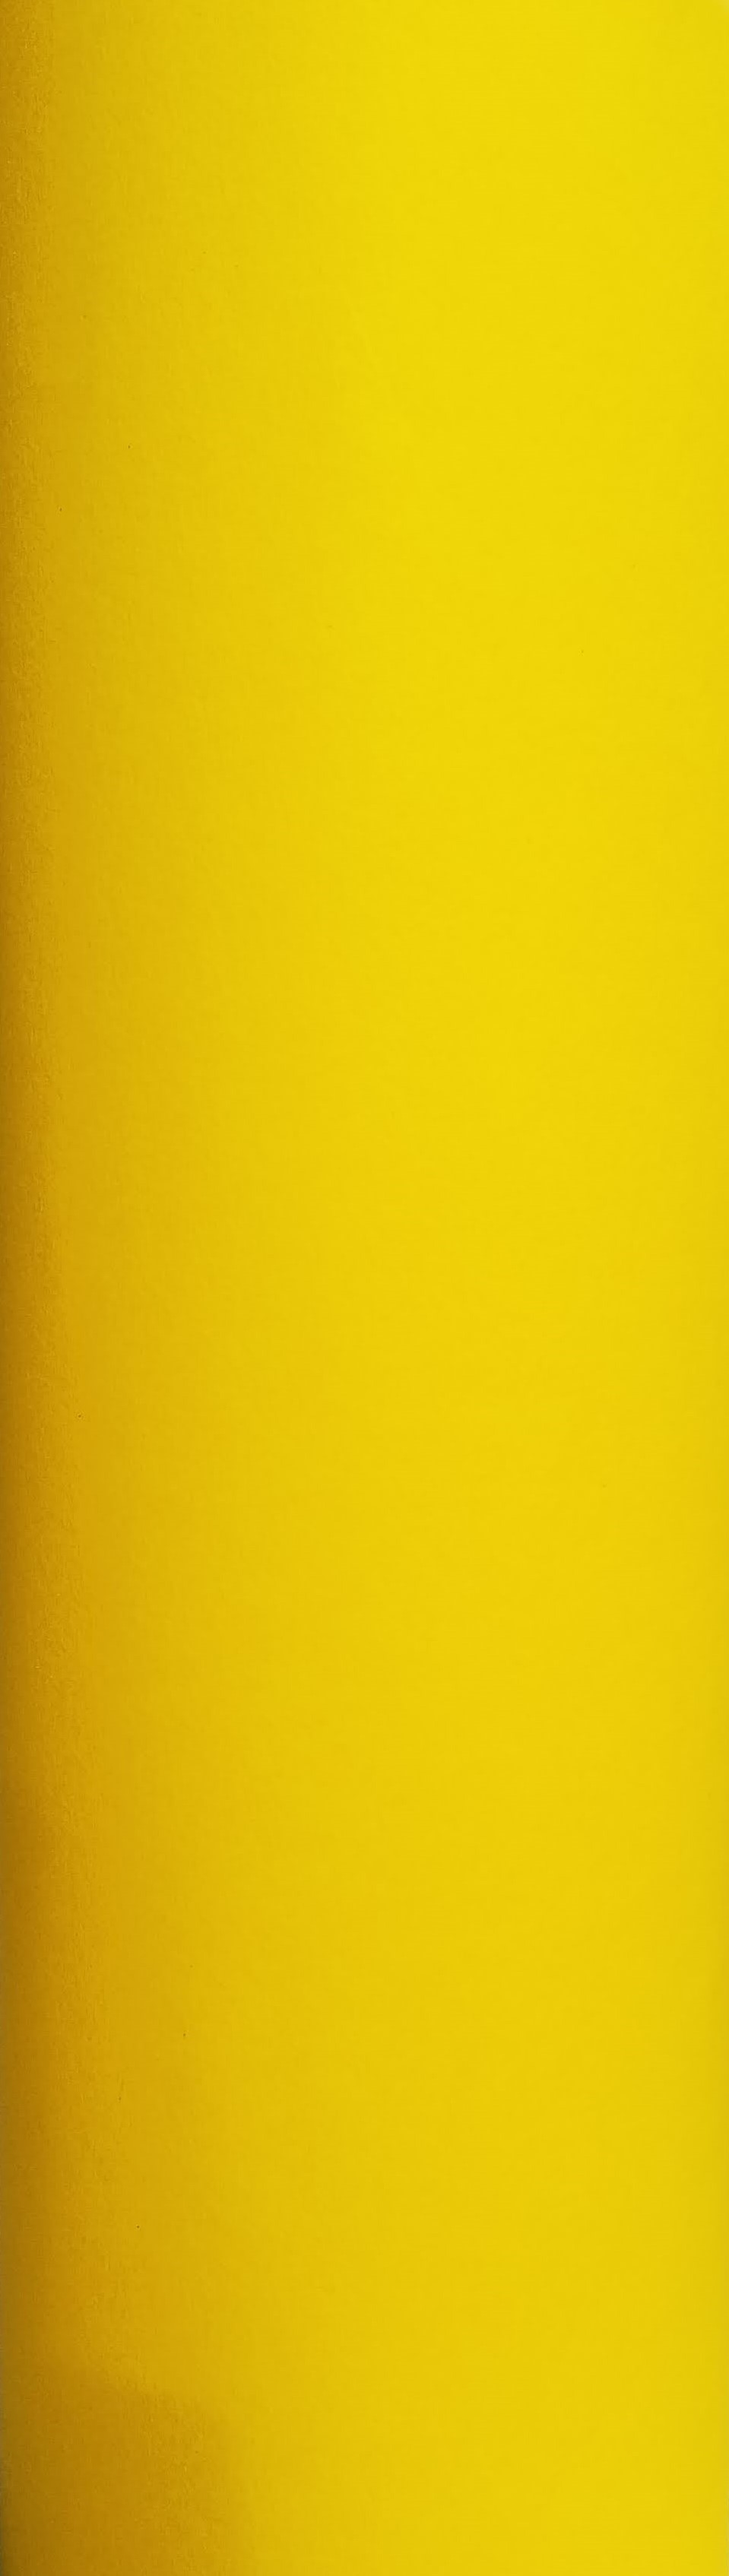
\includegraphics[width=.08\linewidth]{images/test_cut_03.jpg}
		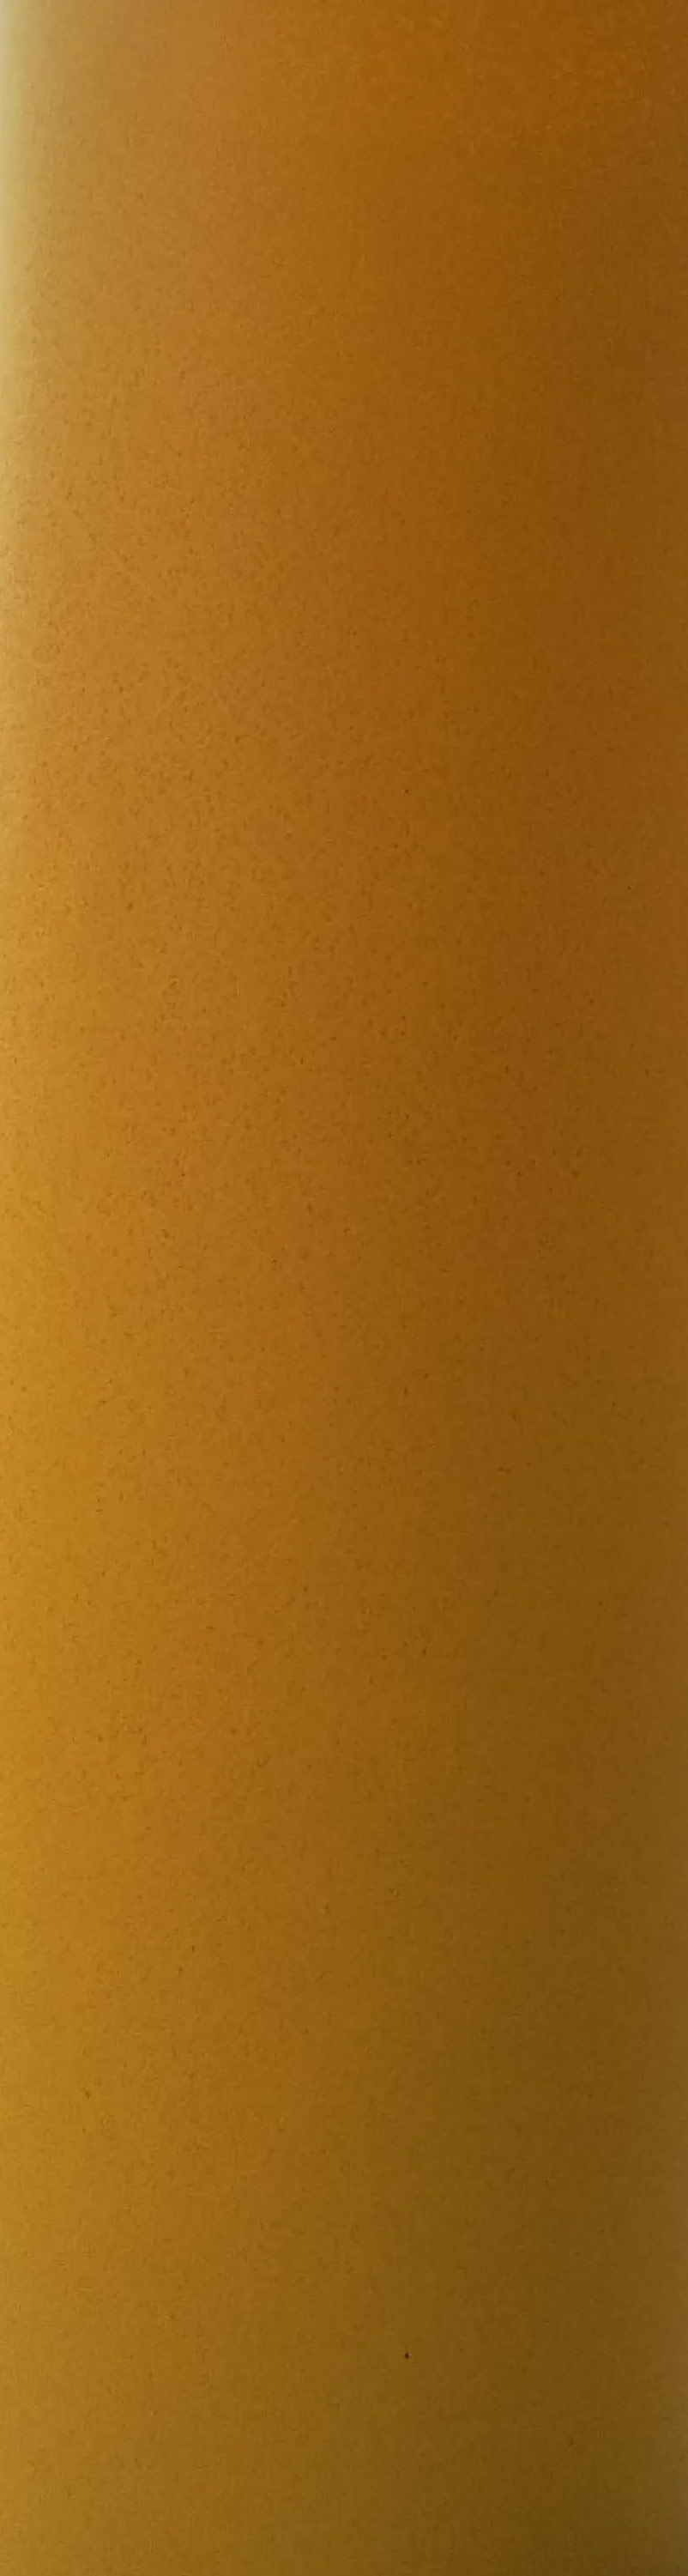
\includegraphics[width=.08\linewidth]{images/test_cut_04.jpg}
		
\includegraphics[width=.08\linewidth]{images/test_cut_05.jpg}
		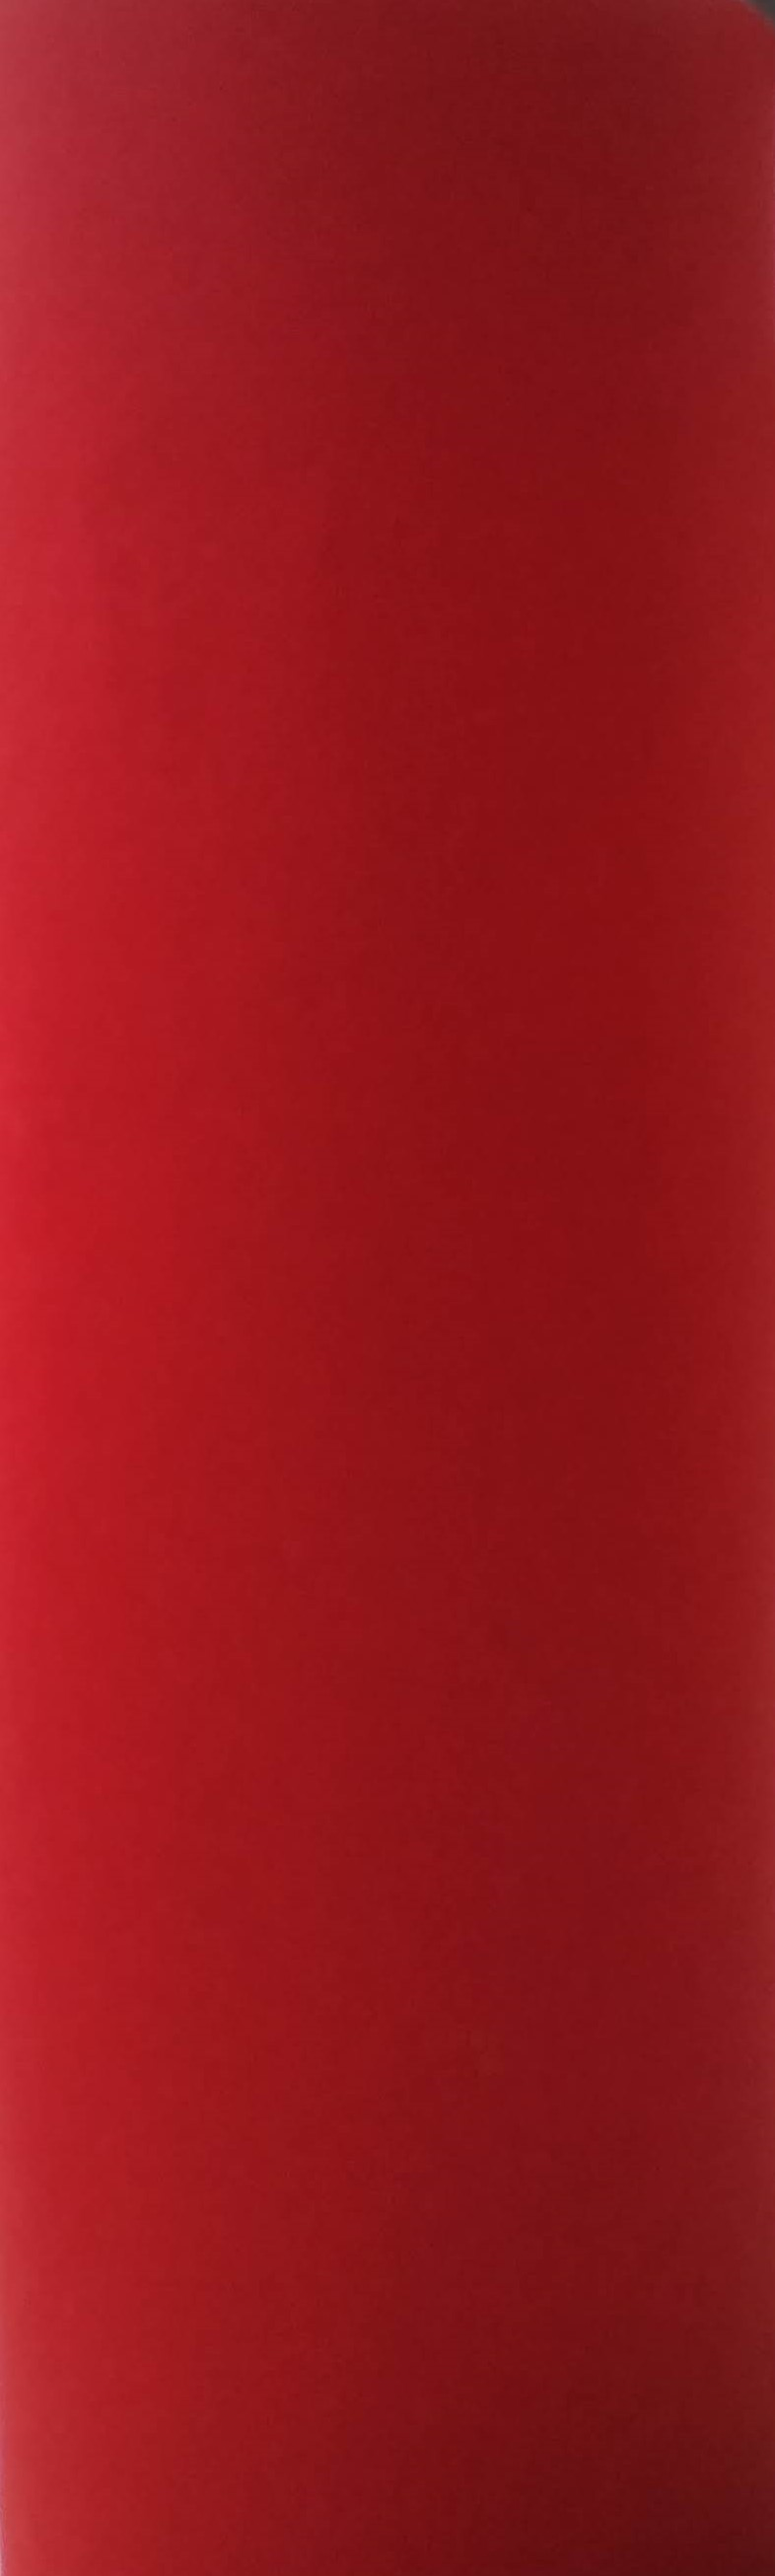
\includegraphics[width=.08\linewidth]{images/test_cut_06.jpg}
		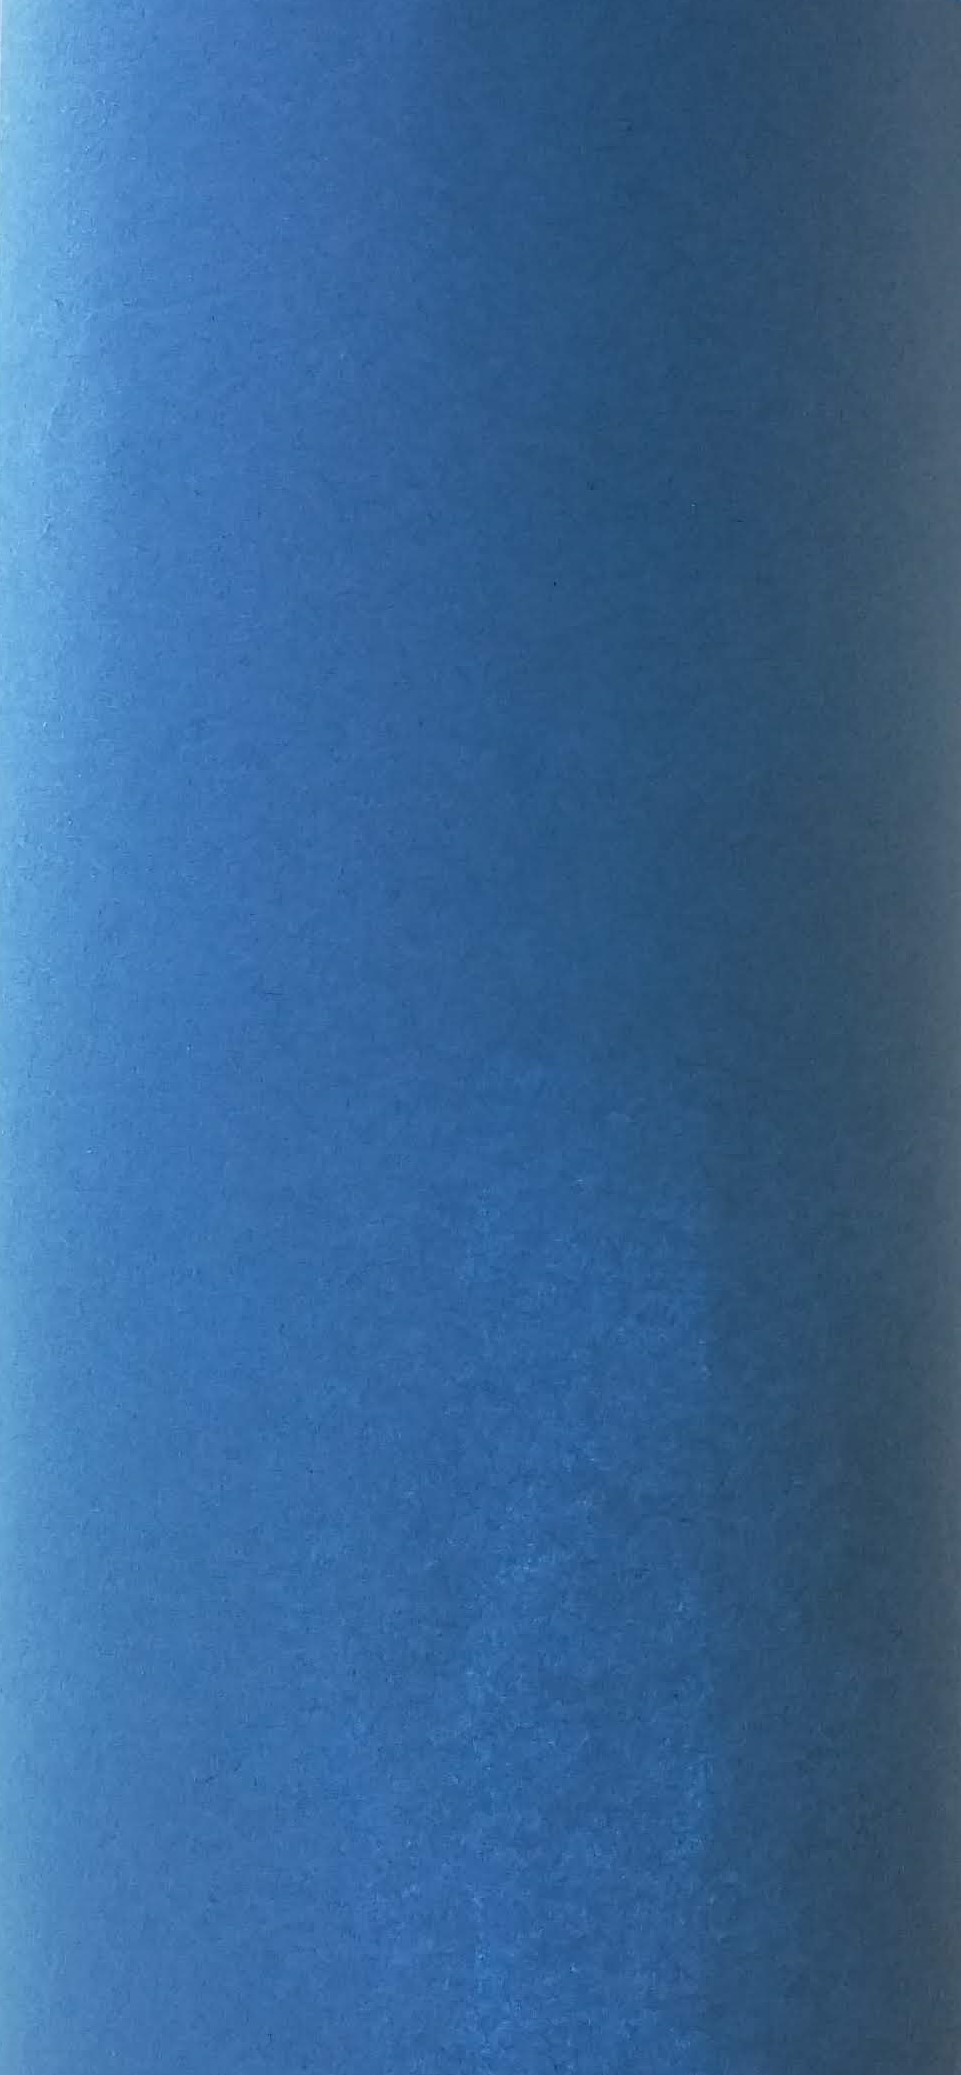
\includegraphics[width=.08\linewidth]{images/test_cut_07.jpg}
		
\includegraphics[width=.08\linewidth]{images/test_cut_08.jpg}
		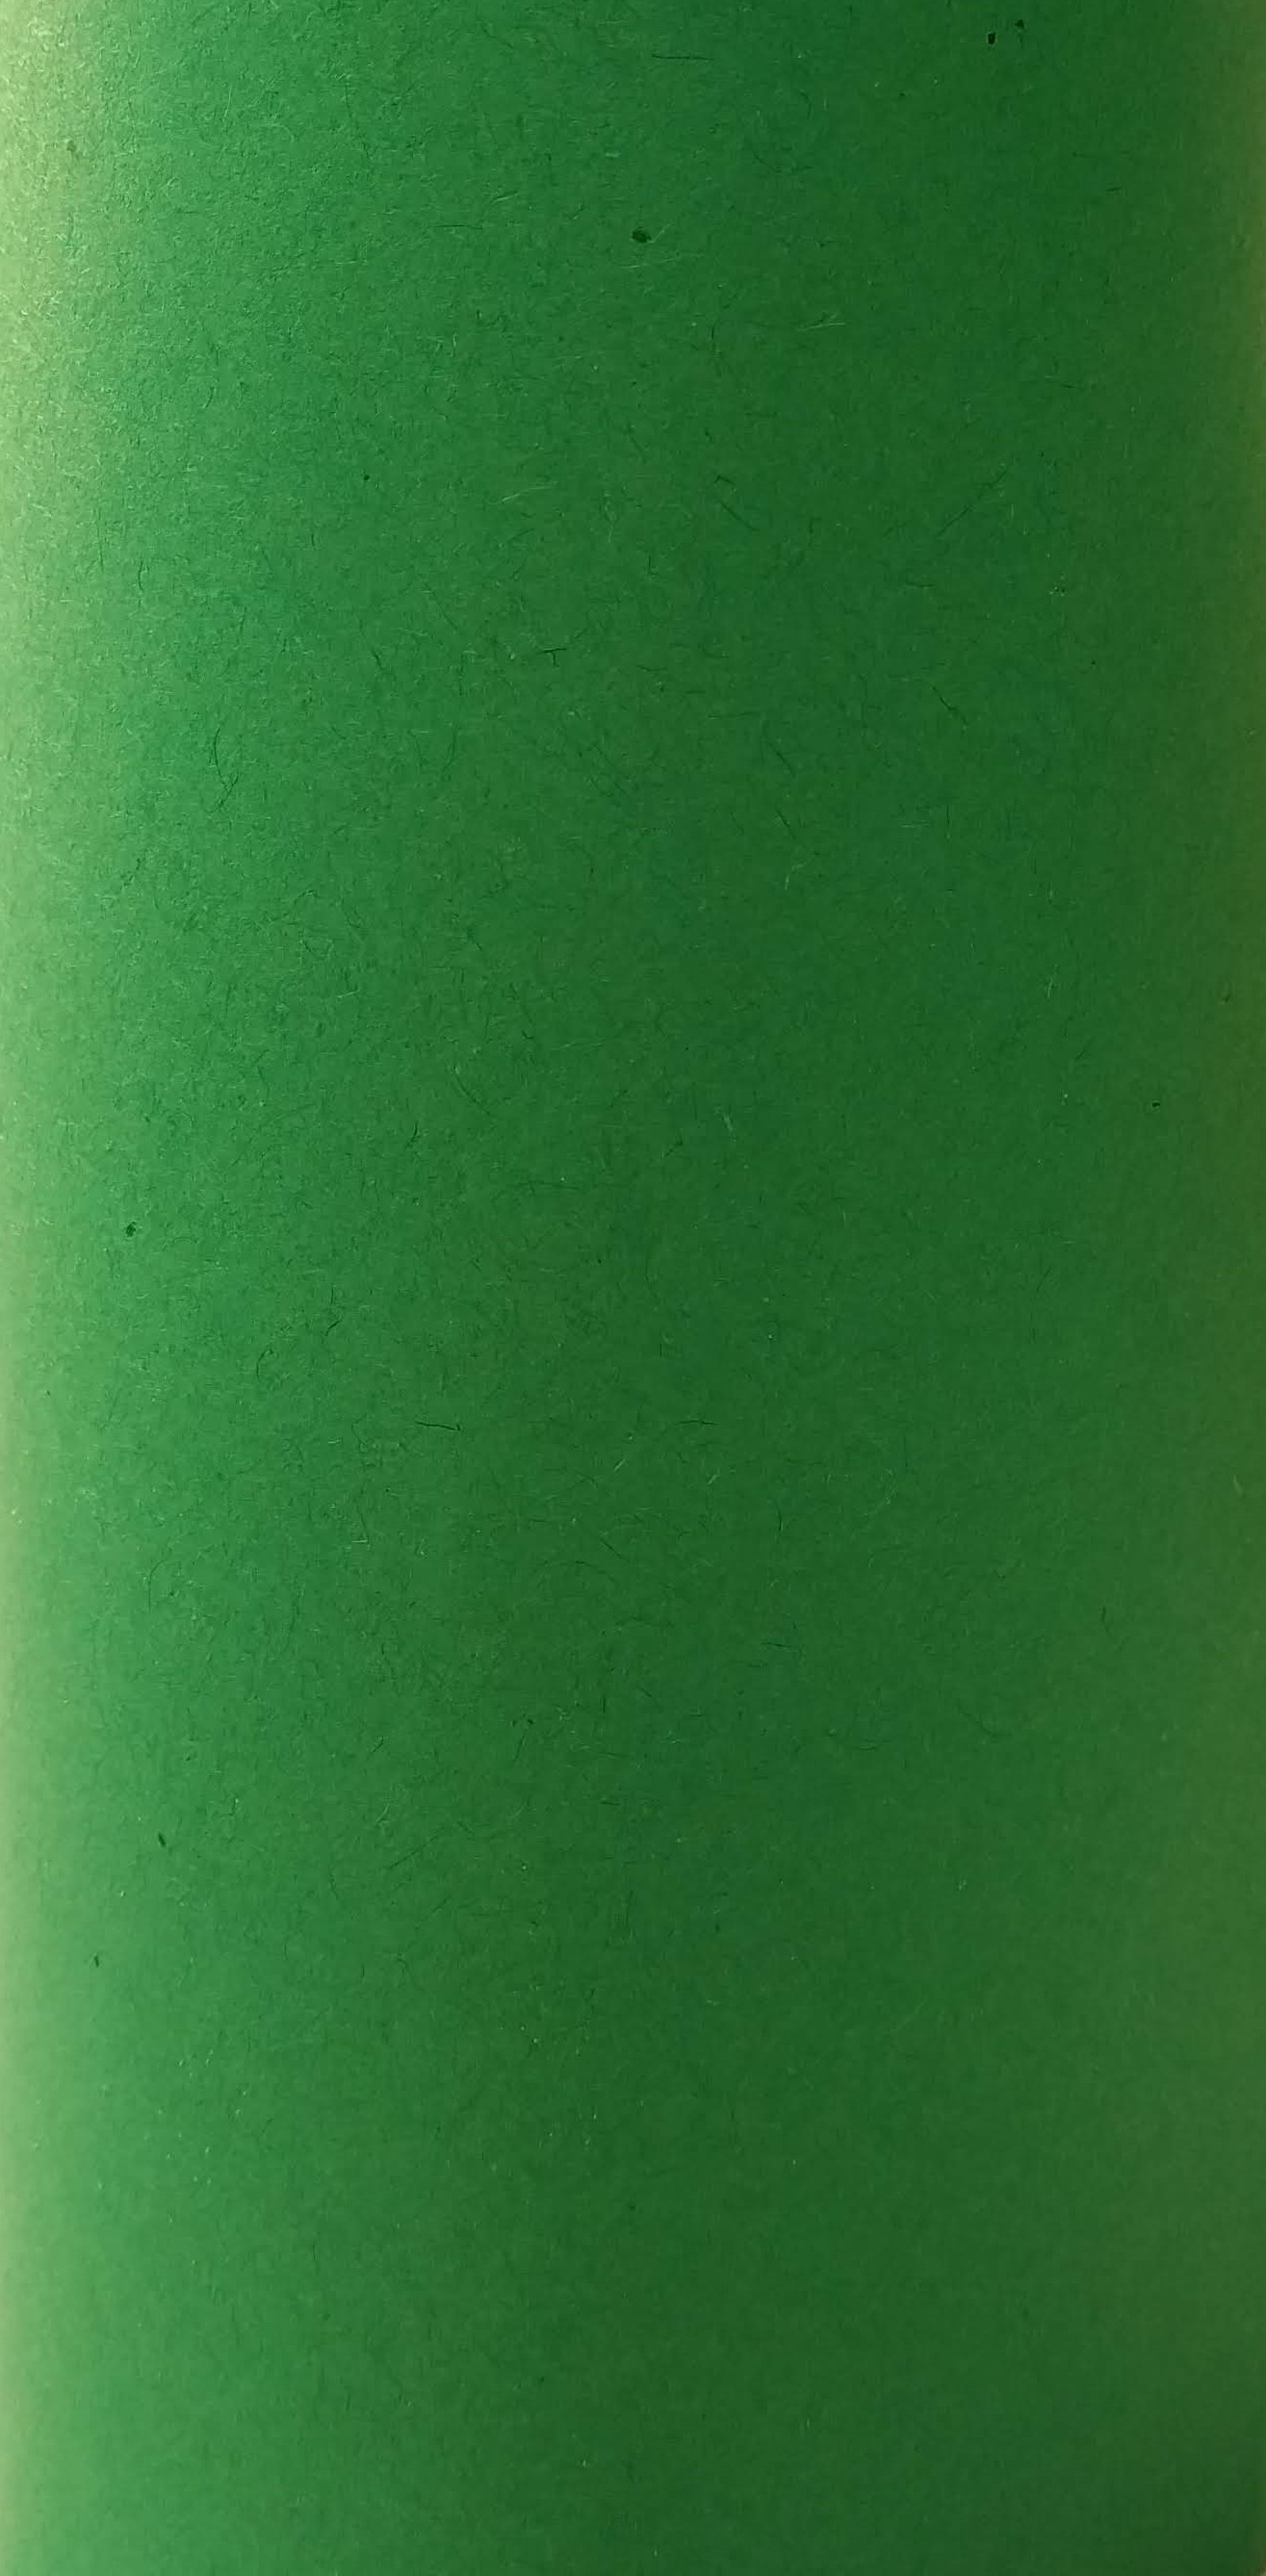
\includegraphics[width=.08\linewidth]{images/test_cut_09.jpg}
		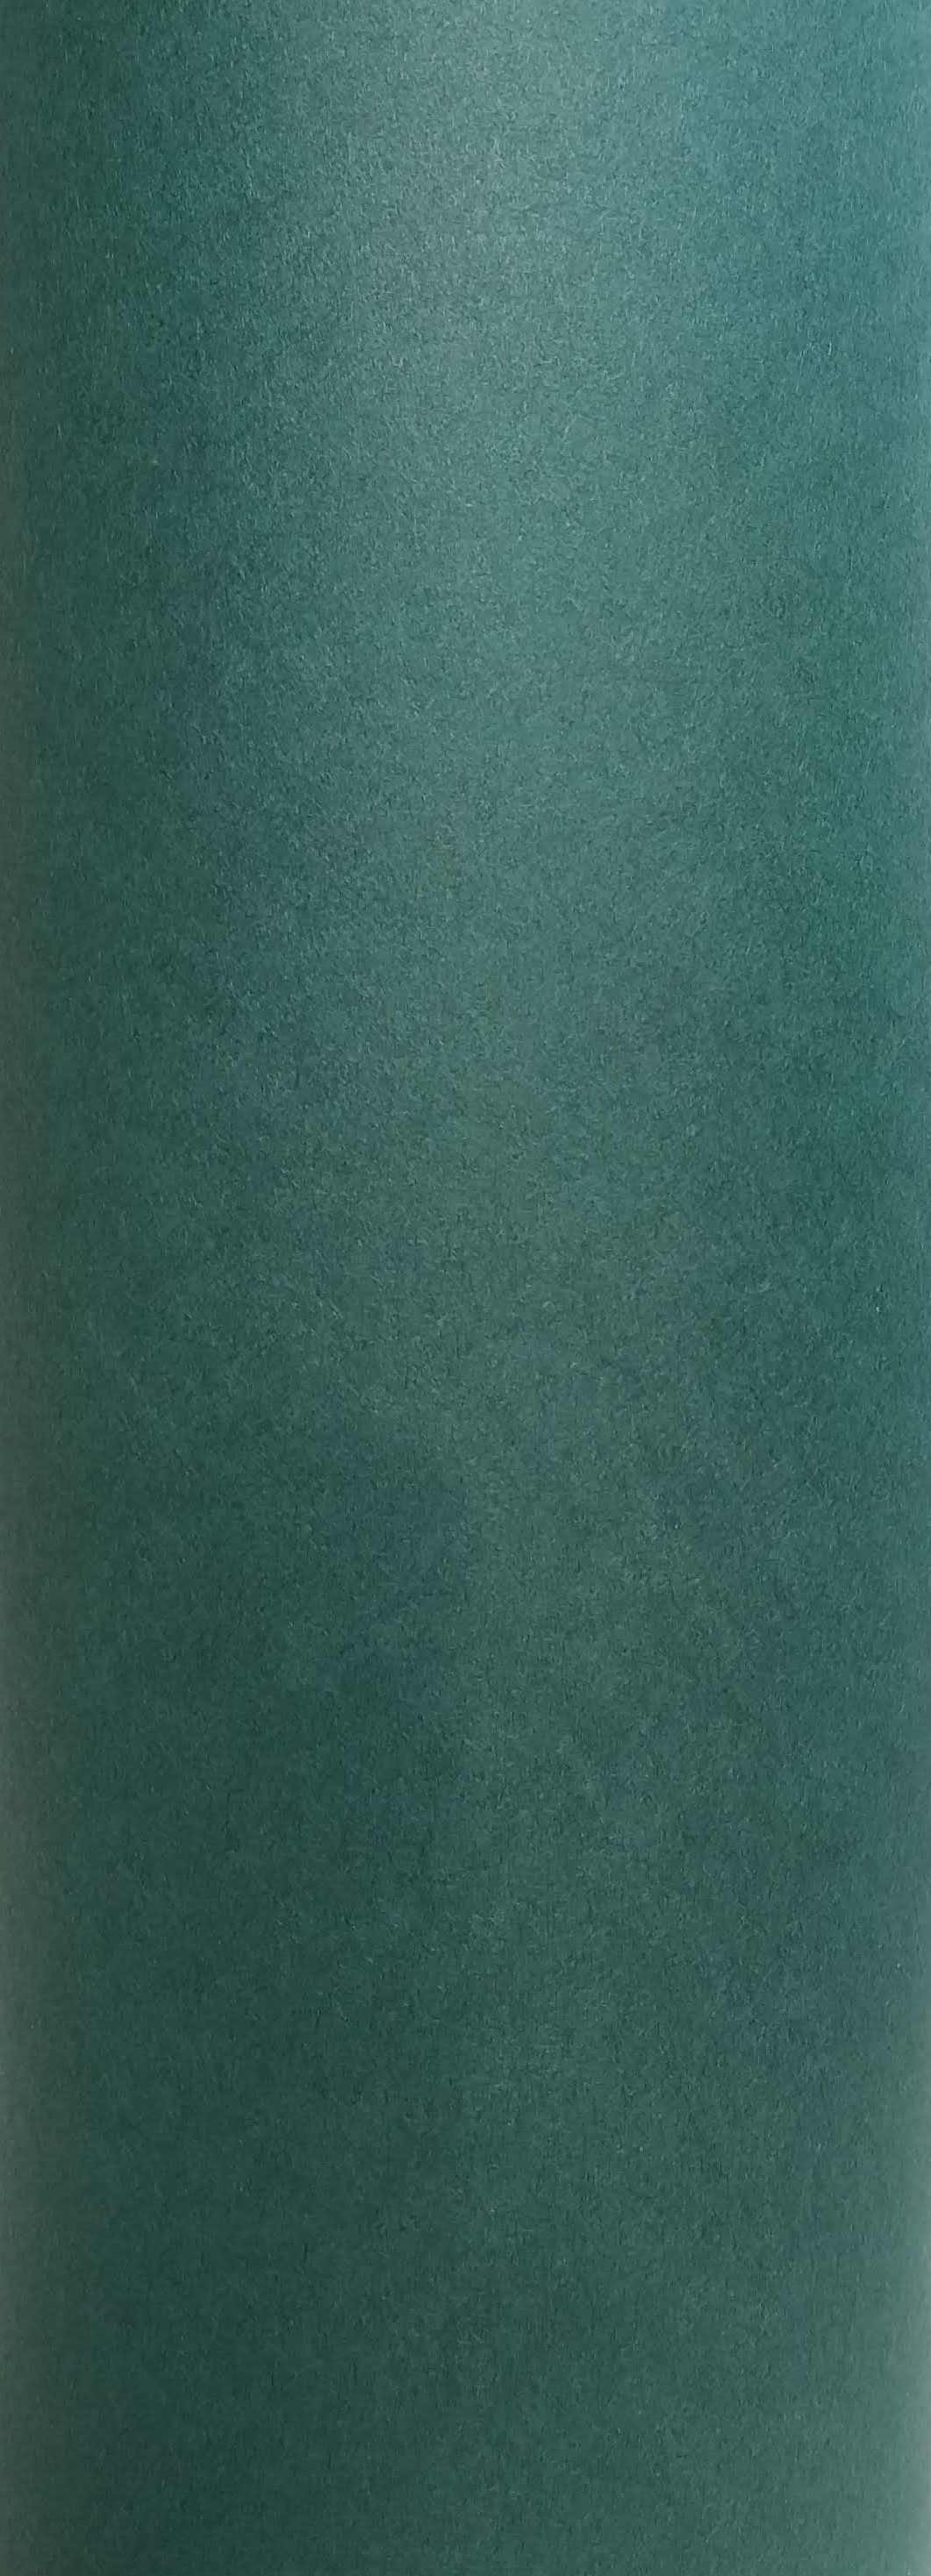
\includegraphics[width=.08\linewidth]{images/test_cut_10.jpg}
		
\includegraphics[width=.08\linewidth]{images/test_cut_11.jpg}
		\caption{Cropped images from testing set}
	\end{figure}

	These cropped images illustrate very well, why we chose to use cylindrical objects as our test set. Each image contains various shades of the colour which is consequence of light hitting different spots on cylinders at different angle. Another reason for choosing this shape is that we expect encountering similar objects in the task2. 
	
	\section{Colour classification}
	
	Our first approach was training a classifier with colours as input vectors. Each colour in colour space can be represented by a vector $v$ and the classification task is to map this vector $v$ to correct class. \\
	
	In the \texttt{RGB} colour space, each vector $v$ can be represented using $v = (red, green, blue)$, where $red, green, blue \in [0, 255]$. \\
	
	To prepare training data set, we used Hough transformation to detect circles in our images and randomly sampled points inside found circles to obtain RGB vectors corresponding to colours. Instead of sampling colour just from one point in the circle, we averaged colours in a region around sampled point. We chose multiple points from the same circle because object's illumination is almost never uniform. \\
	
	In the figure below we have plotted colours from our training set in \texttt{RGB} and \texttt{HSV} colour space. As we can see, in the \texttt{RGB} colour space, the shades of the same colour lie on the same line. Similar thing happens in \texttt{HSV} color space, but the lines are vertical. Because the \texttt{HSV} colour space is conical, the red colour lies both on the far left and far right of our graph. This is not ideal for knn or linear support vector machines, so we predict that those will perform better on the \texttt{RGB} colour space. \\
	
	The \texttt{RGB} and \texttt{HSV} are not natural colour spaces for humans. If two colours are close in \texttt{RGB} space (using euclidean distance), that doesn't mean that human perceive them as similar. There are some colour spaces that are more suited for human perception, for example the \texttt{XYZ} colour space. \\
	
	% Because the input to our classifier is a simple three dimensional vector, we predict that the knn classifier will perform quite well.	
	
	% ZAMENJAJ SLIKO KO DODAŠ ŠE BELO BARVO!
	\begin{center}
		\begin{figure}[H]
			\begin{subfigure}{.5\linewidth}
				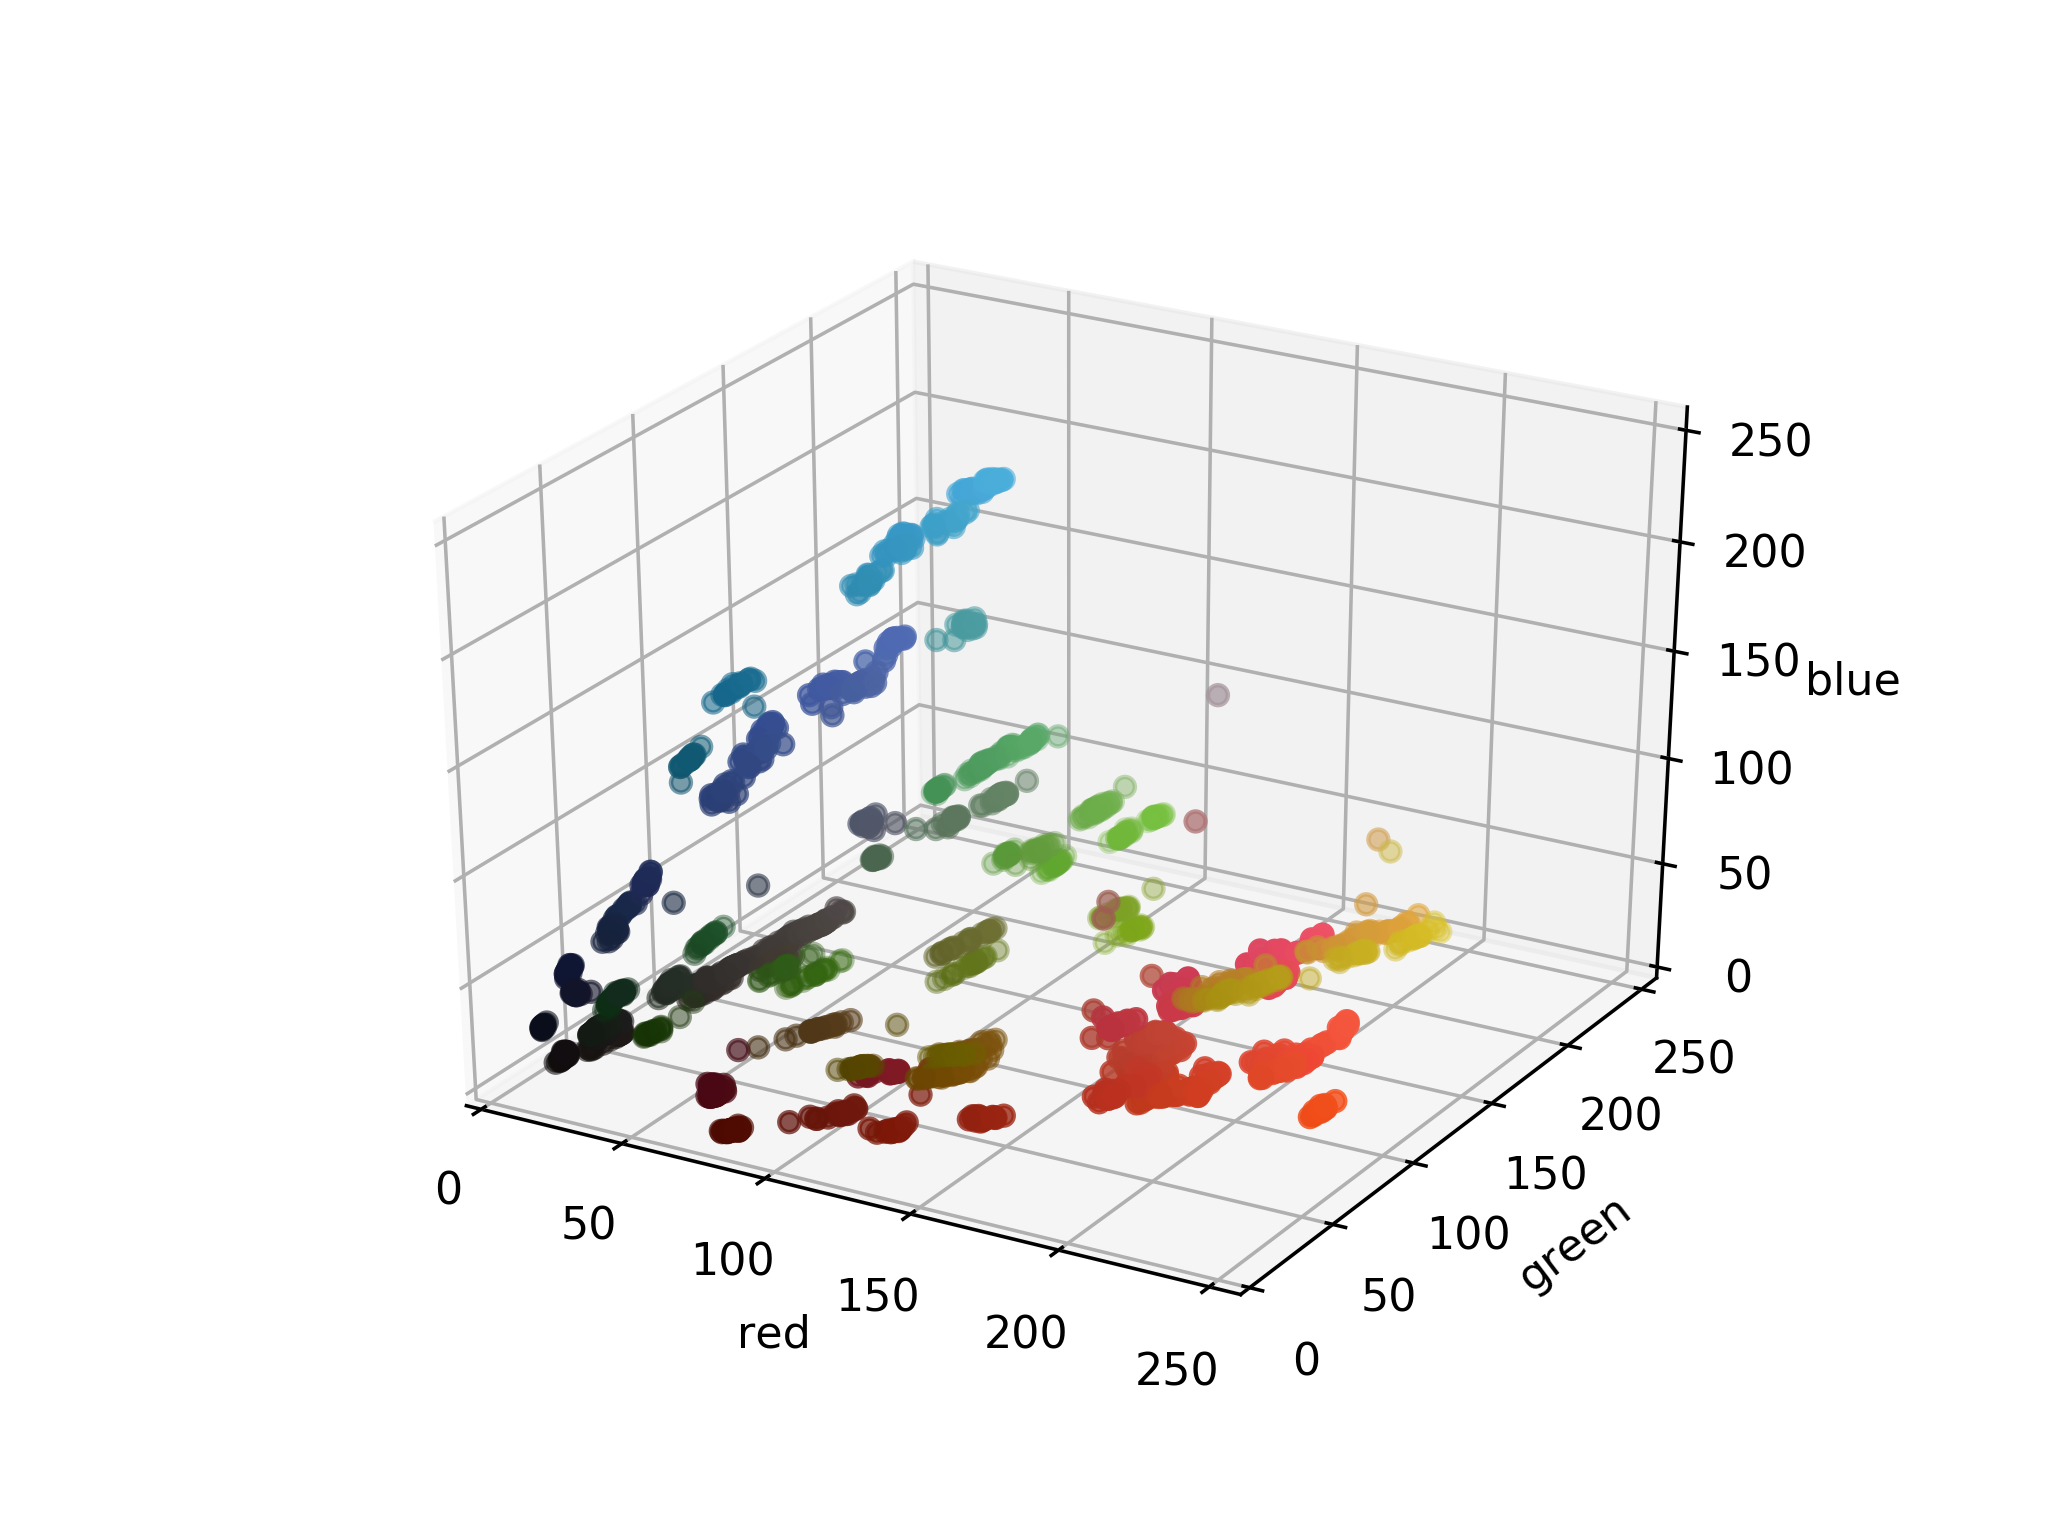
\includegraphics[width=\linewidth]{images/rgb.png}
				\caption{RGB color space}
			\end{subfigure}
			\begin{subfigure}{.5\linewidth}
				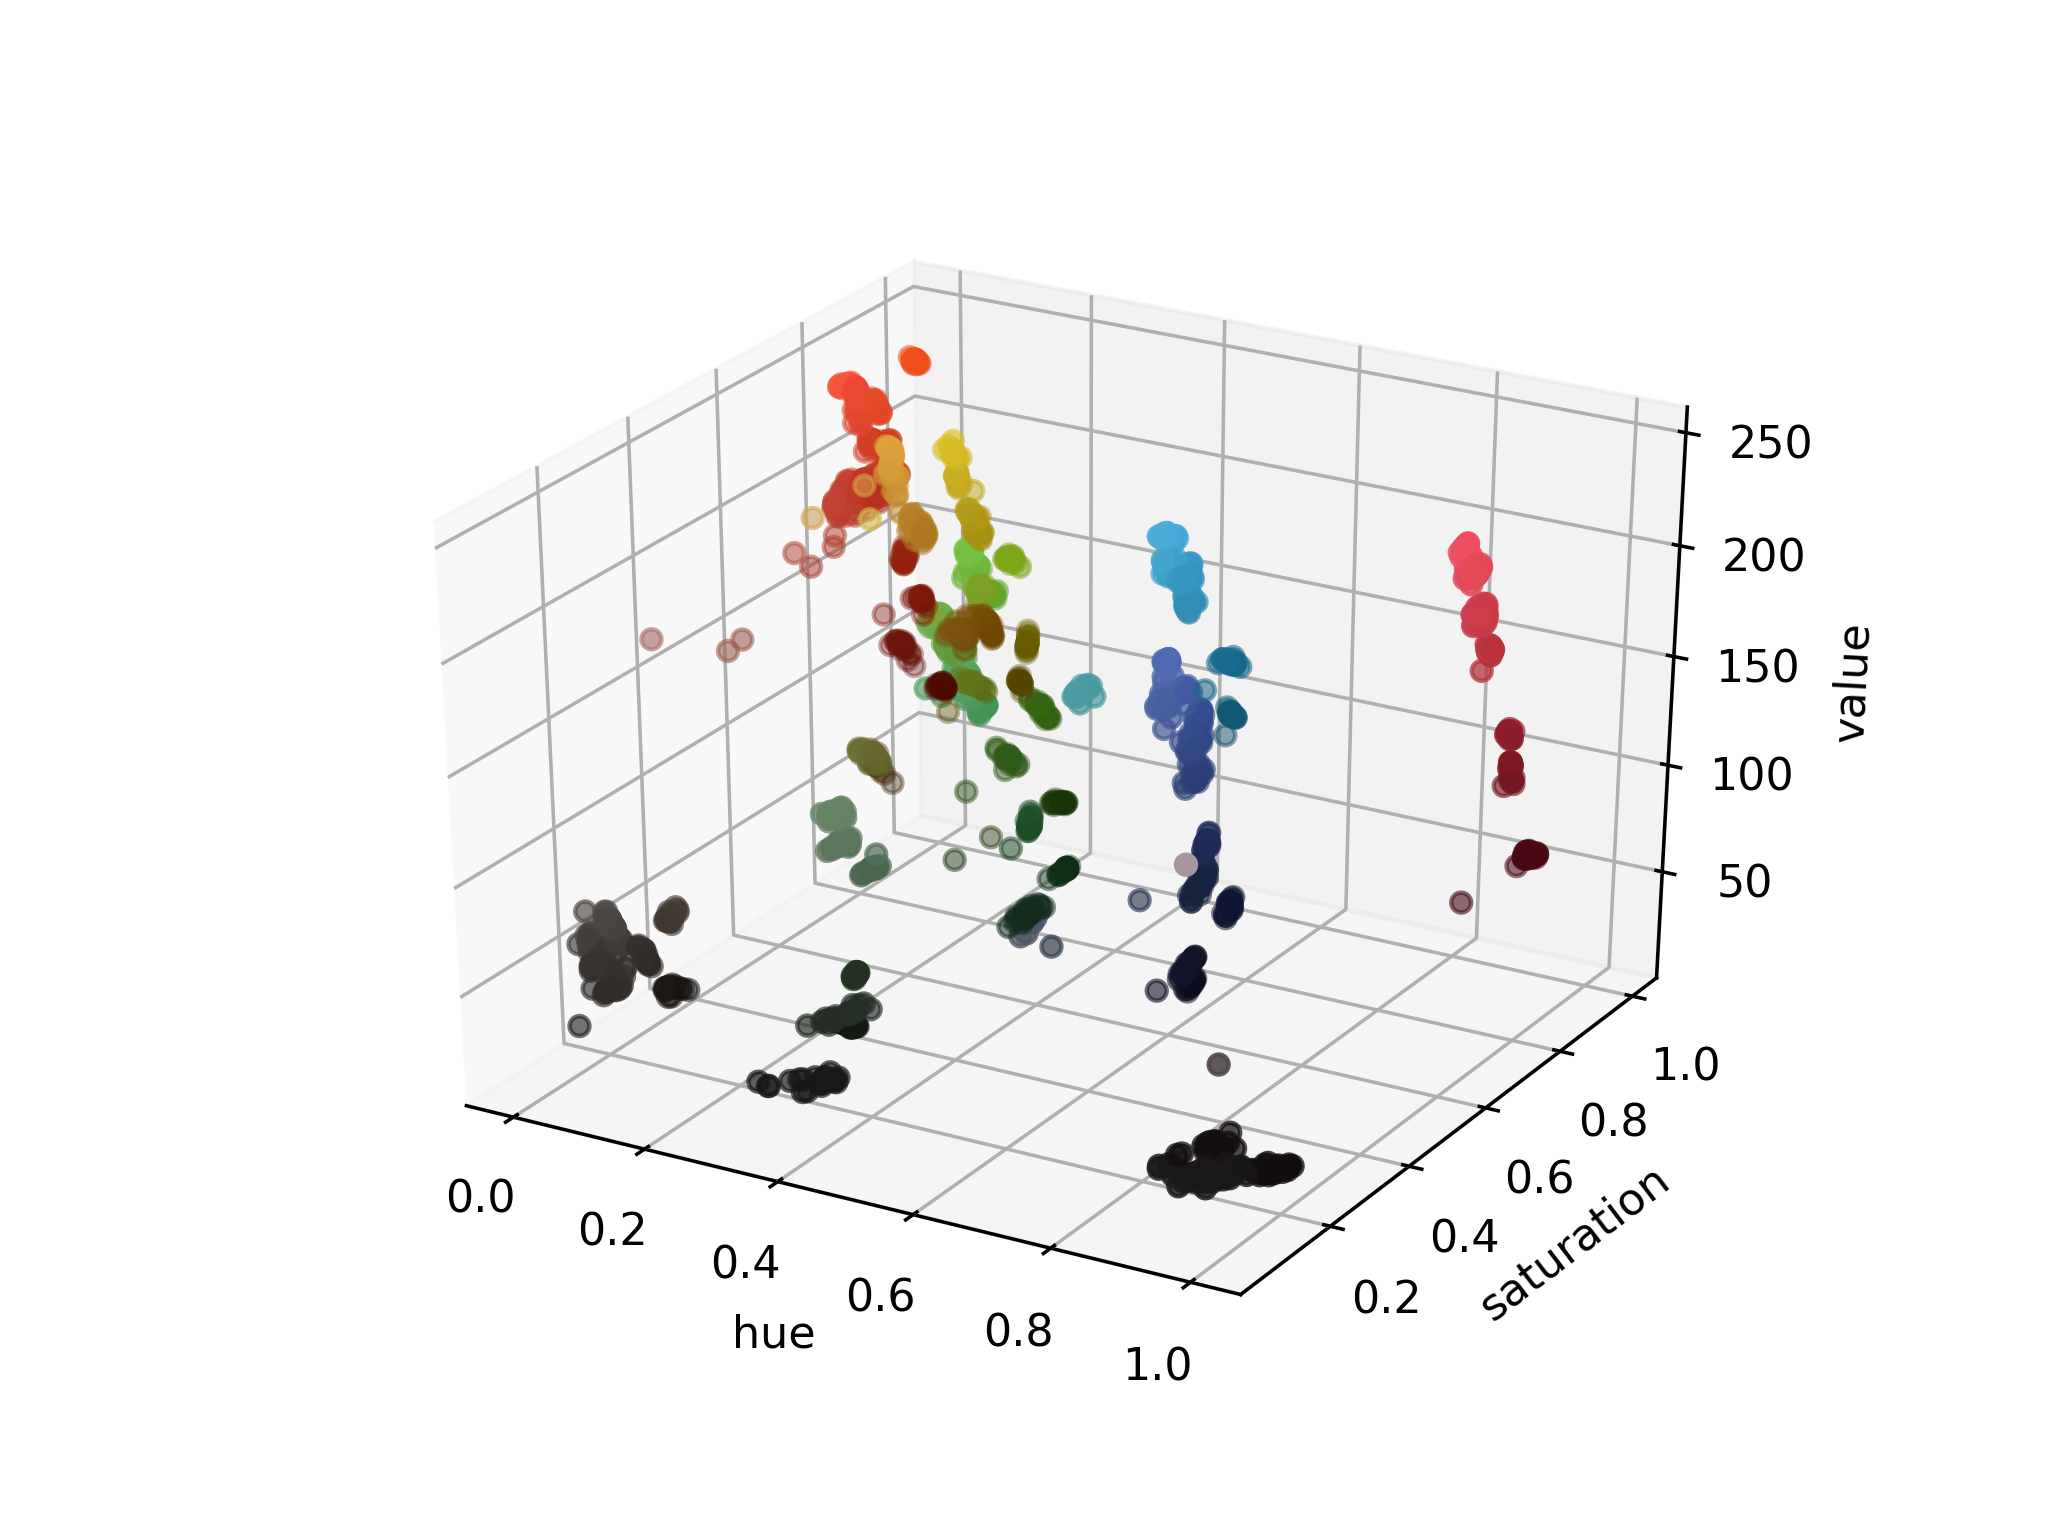
\includegraphics[width=\linewidth]{images/hsv.png}
				\caption{HSV color space}
			\end{subfigure}
		\end{figure}
	\end{center}

	We then tested different classifiers using training data set. Results can be found in the table below. Accuracy is measured using our testing set and is calculated for both \texttt{RGB} and \texttt{HSV} colour space.
	
	\begin{center}
		\begin{tabular}{|c|c|c|c|}
			\hline 
			\textbf{Classifier} & \texttt{RGB} & \texttt{HSV} & \texttt{LAB} \\
			\hline
			knn, k = 1 & 0.88 & 0.52 & 0.94 \\ \hline
			knn, k = 1, weights = distance & 0.88 & 0.52 & 0.94 \\ \hline
			knn, k = 3 & 0.89 & 0.51 & 0.94 \\ \hline
			knn, k = 3, weights = distance & 0.89 & 0.52 & 0.94 \\ \hline
			knn, k = 5 & 0.89 & 0.53 & 0.94 \\ \hline
			knn, k = 5, weights = distance & 0.89 & 0.52 & 0.94 \\ \hline
			knn, k = 7 & 0.90 & 0.52 & 0.94 \\ \hline
			knn, k = 7, weights = distance & 0.90 & 0.53 & 0.94 \\ \hline
			decision tree, gini & 0.80 & 0.88 & 0.86 \\ \hline
			decision tree, entropy & 0.82 & 0.87 & 0.85 \\ \hline
			random forest, gini & 0.85 & 0.82 & 0.91 \\ \hline
			random forest, entropy & 0.82 & 0.85 & 0.89 \\ \hline
			naive bayes & 0.71 & 0.87 & 0.96 \\ \hline
			support vector machine, kernel=linear, c=0.025 & 0.92 & 0.61 & 0.92 \\ \hline
			support vector machine, kernel=rbf, c=0.025 & 0.26 & 0.42 & 0.27 \\ \hline
			support vector machine, kernel=linear, c=0.05 & 0.92 & 0.62 & 0.93 \\ \hline
			support vector machine, kernel=linear, c=0.1 & 0.92 & 0.50 & 0.93 \\ \hline
			support vector machine, kernel=linear, c=0.2 & 0.92 & 0.57 & 0.93 \\ \hline
		\end{tabular} \\
	\end{center}

	As we have predicted, the accuracy in \texttt{HSV} color space is lower than that in the \texttt{RGB} space. \\
	
	% MANJKA IZBOR NAJBOLJŠEGA KLASIFIKATORJA
	
	% ZA VSAK KLASIFIKATOR NAPIŠI OPOMBO ZAKAJ JE TAKO
	
	% OPOMBA GLEDE TEGA, DA JE POTREBNO IZ OBROČKA DOBITI PRAVO BARVO.
	As we can see from the table above, this type of classification works well. The only problem is that we have to choose points on our object, which can sometimes be problematic. But if we sample multiple points, the probability that our classification will be correct increases.	
	
	\section{Convolutional neural network}
	
	The other approach that we tried was training our classifier using entire image of an object. In this case, we don't have to manually sample points on our object. Before we do that, we have to isolate the object and reduce image size. Having a resolution of \texttt{30px x 30px} means that we have 900 inputs to our neural network. Another problem with convolutional neural networks is that we need a large dataset of images, which we don't have in our case. We only have 200 images for all six colours but we would probably need 200 images for each colour. \\
	
	So the first step is to resize our object image to a smaller size to reduce the number of inputs to our classifier. We then reshape our image to one dimensional array and send it to our classifier.
	
	
	
\end{document}